%% FalCom: An MCMC Sampler for Hierarchical Capacitated Facility Location
%% Target: European Journal of Operational Research (EJOR)

\documentclass[11pt]{article}

%% -----------------------------------------------------------------------
%% Packages
%% -----------------------------------------------------------------------
\usepackage[margin=1in]{geometry}
\usepackage{amsmath, amsthm, amssymb}
\usepackage{placeins}
% Float placement: keep figures and tables near their text (article build).
\renewcommand{\topfraction}{0.9}\renewcommand{\bottomfraction}{0.6}
\renewcommand{\textfraction}{0.07}\renewcommand{\floatpagefraction}{0.75}
\setcounter{topnumber}{3}\setcounter{bottomnumber}{2}\setcounter{totalnumber}{5}
\usepackage{graphicx}
\usepackage{subcaption}
\PassOptionsToPackage{hyphens}{url}
\usepackage[hidelinks]{hyperref}
\usepackage{enumitem}
\usepackage{booktabs}
\usepackage{multirow}
\usepackage{xcolor}
\usepackage[numbers,sort&compress]{natbib}
\usepackage[expansion=false]{microtype}
\usepackage[ruled]{algorithm2e}
\usepackage{tikz}
% Line numbering for collaborative review. Every line numbered;
% mathlines extends numbering into display math.
% Remove these two lines before final submission.
\usepackage[mathlines]{lineno}
\usetikzlibrary{arrows.meta, backgrounds, decorations.pathreplacing, fit, positioning, shapes.geometric}
%% -----------------------------------------------------------------------/Users/kirtisoglu/.athenaeum/overleaf/pmnck5g5r/literature/falcom.tex
%% Theorem environments
%% -----------------------------------------------------------------------
\newtheorem{theorem}{Theorem}[section]
\newtheorem{proposition}[theorem]{Proposition}
\newtheorem{lemma}[theorem]{Lemma}
\newtheorem{corollary}[theorem]{Corollary}
\newtheorem{claim}[theorem]{Claim}
\theoremstyle{definition}
\newtheorem{definition}[theorem]{Definition}
\newtheorem{remark}[theorem]{Remark}
\newtheorem{assumption}[theorem]{Assumption}

%% -----------------------------------------------------------------------
%% Custom commands
%% -----------------------------------------------------------------------
\newcommand{\Pc}{\mathcal{P}}          % partition
% (\Fc macro removed: candidate sets are written F^\ell)
\newcommand{\Cc}{\mathcal{C}}          % constraints
% \Omega already defined by amssymb
% \newcommand{\mub}{\mu_\beta}         % Boltzmann measure (removed)
\newcommand{\dbar}{\bar{d}}            % average demand
\DeclareMathOperator{\Contiguity}{Contiguity}  % closed-form contiguity predicate
\DeclareMathOperator*{\argmax}{arg\,max}
\newcommand{\TODO}[1]{{\color{red}[TODO: #1]}}
\newcommand{\NOTE}[1]{[Note: #1]}
% Wraps any text/equation that would need to change if we convert the
% main-text parametrization from \varepsilon to \tau (see appendix
% "Direct tolerance parametrization $\tau$"). Flip the body to {#1}
% once the conversion is committed.
\newcommand{\epsfix}[1]{#1}
% \DESIGN flags a modeling choice the author wants to decide on; the
% bracketed alternatives are highlighted in orange and survive only
% until the design call resolves them.
% (DESIGN macro removed)
% \NEXT flags an outstanding follow-up task (green so it visually
% separates "what still needs running" from \TODO drafting holes).
\newcommand{\NEXT}[1]{{\color{teal}[NEXT: #1]}}

%% -----------------------------------------------------------------------
\begin{document}
\linenumbers
%% -----------------------------------------------------------------------

\title{FalCom: An MCMC Sampling Framework for Facility Location and Districting Problems}
\author{Alaittin K\i rt\i \c{s}o\u{g}lu$^1$ and Hemanshu Kaul$^1$}

\footnotetext[1]{Department of Applied Mathematics, Illinois Institute 
of Technology, Chicago, IL 60616. E-mail: {\tt {kaul@iit.edu, kirtisoglu@hawk.iit.edu}}}

\date{}

\maketitle

\begin{abstract}
    Districting partitions geographic areas into balanced, contiguous, and compact 
    service districts. Recent advances in political redistricting have demonstrated 
    the potential of recombination-type Markov chain Monte Carlo (MCMC) methods for 
    exploring the space of feasible districting plans and revealing structural 
    alternatives. The hierarchical capacitated facility location problem, in 
    contrast, concerns facility placement and demand allocation across multiple 
    service levels, subject to capacity constraints, but does not generally require 
    districts to be contiguous.

    In this paper, we introduce \emph{FalCom} (Facility Location Combination), a 
    recombination-type MCMC sampler for hierarchical districting with capacitated 
    facility assignments. FalCom partitions a geographic region at two hierarchical levels, assigns a facility and an integer capacity to every district, and lets the number and sizes of districts emerge within a total capacity fixed by the demand. We validate FalCom against exact enumeration on small 
    instances and evaluate its computational scaling on synthetic grids with up 
    to $50{,}000$ basic units. Run as an annealing optimizer on grids of $100$ and $400$ basic units, FalCom reaches states within $1\%$ and, with a larger budget, $4\%$ of proven optima of the mixed-integer model, with the same capacity mix and level-2 facilities and, up to one site, the same open level-1 facilities, as the best of eight annealing runs under a slightly wider balance tolerance than the model's. 
    Finally, we apply FalCom to the London Ambulance Service, using data on its $66$ 
    real ambulance stations. The resulting ensemble characterizes the variation of response-area boundaries, station workloads and operational groupings under the sampler's law, and provides a reference distribution against which the existing service layout is read.
\end{abstract}


\section{Introduction}
\label{sec:intro}
%% -----------------------------------------------------------------------

% ---- 1. What is districting ----
Districting is the problem of grouping small geographic areas, called
\emph{basic units}, into larger geographic clusters, called \emph{districts}, 
subject to three classical planning criteria: \emph{balance}, \emph{contiguity}, 
and \emph{compactness}. Balance requires districts to have nearly equal demand sizes 
with respect to one or more activity measures such as workload, sales 
potential, or population. Contiguity requires that any two basic units within a 
district can be connected by a path that remains entirely within the district, 
while compactness favors districts that are relatively round-shaped. Depending on 
the application,  districting is also referred to as territory design, zone design, 
or territory alignment.


% ---- 2a. Applications of districting ----
Districting provides a common framework for partitioning geographic areas, 
although the relative importance of its planning criteria varies across 
applications. Political redistricting partitions a territory into a fixed 
number of districts with approximately equal populations for electoral 
purposes~\citep{ricca2013political}. Sales territory design assigns customers 
to sales representatives while balancing sales potential or 
workload~\citep{kalcsics2005towards}. Service districting defines service areas 
for schools, police patrols, and home-care teams, with balance measured in terms 
of student attributes, crime rates, and patient workloads, 
respectively~\citep{blais2003solving, camacho2015multi, bouzarth2018assigning}. 
Distribution districting creates delivery zones for postal services, meter reading 
and last-mile routing problems~\citep{ramirez2023reconfiguration, de2014redistricting, 
sandoval2022novel}. Despite their different operational objectives, these 
applications share the challenge of constructing geographically coherent districts 
while balancing competing planning criteria. A comprehensive survey of districting 
problems and their applications is provided by~\citet{CAMPOSVALDES2026103654}.

% ---- 2b. Why districting matters ----
The quality of a districting plan has direct consequences for both the populations 
served and the organizations delivering services. Poorly balanced districts can 
overwhelm some service teams while leaving others underutilized, degrading response 
times and increasing operational costs. Non-contiguous or elongated districts can 
also increase travel distances for sales representatives, delivery vehicles, patrol 
officers, and home-care nurses~\citep{kalcsics2020districting}. In healthcare, 
district boundaries determine which communities are assigned to each care team and 
can influence geographic disparities in access to services. In emergency services, 
the design of service areas can affect travel times and, consequently, how quickly 
responders reach those in need. Moreover, districting changes entail administrative 
transition costs, including staff retraining, caseload reassignment, information-system
updates, and coordination among organizations. These consequences motivate principled 
methods for systematically exploring feasible districting plans rather than relying 
on a single design that may overlook important alternatives.

% ---- 3. The facility connection ----
In many applications, determining which customers should be grouped into a district 
is only part of the planning problem; decision-makers may also need to determine 
where to locate the facilities that serve those customers. Districting and facility 
location are often studied separately, in part because jointly optimizing these 
decisions can be computationally challenging~\citep{kalcsics2005towards}. Nevertheless, 
\citet{kalcsics2020districting} emphasize the importance of customer 
allocation in location problems, observing that ``equally important is the second 
aspect of location problems that is usually not mentioned explicitly: the allocation 
of customers to facilities.'' In capacitated facility location, facilities serve 
assigned customers subject to capacity constraints, while districting additionally 
emphasizes the spatial organization of these assignments, often requiring districts 
to be contiguous. This connection creates opportunities for transferring modeling 
ideas and solution methods between the two problem classes, particularly when 
contiguity and capacity are central considerations.

% ---- 4. Hierarchy ----
Many real-world systems organize service areas into multiple administrative or service 
levels. In healthcare networks, primary-care districts may be grouped into larger 
regions of patient referrals~\citep{wang2025cluster}, while in public administration, 
municipalities are grouped into counties or provinces~\citep{bruno2017territorial}. 
We refer to these higher-level aggregations as \emph{superdistricts}. Hierarchical 
districting partitions basic geographic units into districts and groups these districts 
into superdistricts, typically imposing balance and contiguity constraints at each 
level. The hierarchical capacitated facility location problem (HCFL), in contrast, 
incorporates facility-location decisions at multiple levels and capacity constraints 
linking assignments across levels, but without necessarily requiring contiguity for the
service areas~\citep{contreras2020hierarchical}. 

% ---- 5. Computational challenge and sampling ----
Districting problems are computationally hard. Enforcing geographic contiguity in an integer program takes either exponentially many cut constraints, separated during branch-and-cut, or a polynomial-size flow formulation with many auxiliary variables~\citep{validi2022imposing}. Exact methods have nonetheless come a long way. For contiguous, population-balanced districts with a compactness objective, branch-and-cut now solves every county-level instance in the United States and some tract-level ones~\citep{validi2022cutedges, validi2022imposing}, and a cut-generation scheme solves commercial territory instances with $5{,}000$ to $10{,}000$ units for one specific model~\citep{rios2013commercial}. The remaining tract-level instances, and models with more structure, are beyond exact methods without decomposition, which is why the largest instances are handled by coarsening the graph and solving exactly only at the coarsest level~\citep{swamy2023multiobjective}, or by metaheuristics, which the survey of \citet{kalcsics2020districting} reviews. Capacitated facilities and a second hierarchical level add decisions that interact with every assignment, and Section~\ref{sec:exp-milp} shows what that costs on our own model: a proven optimum takes a quarter of an hour on a grid of $400$ units with $15$ candidate sites. All of these methods, exact or heuristic, return one plan. Many planning applications would benefit from several. A distribution over plans lets decision-makers investigate trade-offs, assess the stability of assignments and the robustness of facility locations, and identify the features that persist across solutions. The survey of \citet{kalcsics2020districting} calls for a common and generic framework for districting problems in place of application-specific heuristics with yet another compactness measure or balance constraint. This paper takes a step in that direction by developing a framework for sampling hierarchical districting plans at scale while locating capacitated facilities.

% ---- 6. Political redistricting as methodological bridge ----
A promising methodological direction comes from computational political redistricting. 
The Recombination (ReCom) method of \citet{deford2021recombination} uses 
Markov chain Monte Carlo (MCMC) to sample contiguous, population-balanced districting 
plans by repeatedly recombining two adjacent districts and re-splitting their union. 
However, ReCom was developed for political redistricting and does not directly address 
capacity constraints, multiple hierarchical levels, and facility assignments, 
which are considered here in detail.

% ---- 7. Our contribution ----
\paragraph{Our contribution.}
We introduce \emph{FalCom} (Facility Location Combination), a
ReCom-type MCMC sampler for capacitated hierarchical districting
with facility assignment. To our knowledge, FalCom is the first sampler that combines a hierarchy of districts, a facility and an integer capacity in every district, and a variable number of districts. The multiscale merge-split samplers of political redistricting, which work on two levels of geographic units, are its closest predecessors (Section~\ref{sec:lit-districting}).
We summarize FalCom's contributions as follows.
\vspace{2mm}
\begin{enumerate}[nosep, label=(\roman*)]
     \item \textbf{Hierarchical capacitated partitioning.}
        FalCom operates on a multi-level graph structure, enforcing
        capacity and demand balance constraints at each level. Unlike the samplers in political redistricting, which prescribe the number of districts in advance, FalCom fixes the total number of service teams from the demand and lets the number and capacities of districts emerge within that budget: a plan with $k$ teams opens between $k/c^1_{\max}$ and $k$ facilities.


    \item \textbf{Ensemble-based analysis.} FalCom samples feasible hierarchical 
        partitions, enabling distributional analyses of district boundaries, facility
        assignments, and capacity utilization. Boundary frequency maps
        reveal which boundaries recur across sampled plans, facility
        assignment frequencies indicate the stability of assignments
        across the ensemble, and capacity utilization profiles characterize
        the distribution of workloads. This ensemble perspective, developed
        extensively in political redistricting for applications such as
        gerrymandering detection, provides a basis for assessing alternatives 
        beyond a single optimized plan.

    \item \textbf{Scalability.}  We demonstrate that FalCom can run chains on 
        instances with up to $|V| = 50{,}000$ basic units. A step is local at level~1, where it re-cuts one superdistrict, and global at level~2, where it re-partitions the supergraph of $k$ nodes. On the tested grids, where $k$ grows from $5$ to $112$, the median time of an accepted step grows by a factor of $30$ and the mean step including rejected proposals by a factor of about $41$, while $|V|$ grows $500$-fold; at a fixed graph size the cost grows with the team count through the supergraph re-partition (Section~\ref{sec:exp-scalability}).

    \item \textbf{A benchmark for plans obtained by other means.} The ensemble places a given plan, an existing layout or the output of an optimization model, against a reference distribution of feasible plans; Section~\ref{sec:exp-emergency} reads the operational layout of the London Ambulance Service in this way. FalCom does not optimize within districts. Routing, staffing and dispatch models can be applied inside the sampled districts, which we leave to future work (Section~\ref{sec:extensions}).
    \end{enumerate}
\vspace{2mm}

To aid reproducibility of our work, an open-source implementation of FalCom is available online, and a companion repository holds the experiment code, the synthetic instances, the London data assembly and the stored output of every chain reported in Section~\ref{sec:experiments}, with the commands and seeds that produced them~\citep{falcomchain}.


% ---- 8. Paper outline ----
The rest of the paper is organized as follows.
Section~\ref{sec:literature} reviews the related literature. Section~\ref{sec:model} 
introduces the problem formulation and the hierarchical graph structure, while 
Section~\ref{sec:graph} describes the state space and feasibility rules. 
Section~\ref{sec:falcom} presents the FalCom algorithm, including the proposal 
mechanism, recursive partitioning, capacitated tree cuts, and facility assignment 
phase. Section~\ref{sec:convergence} establishes feasibility and states what is known, and what is open, about the chain's convergence, a status it shares with the ReCom family. Section~\ref{sec:experiments} 
validates the sampler against exact enumeration, evaluates its scaling on large 
synthetic grids, compares sampled results with mixed-integer linear programming 
solutions, and presents an application to the London 
Ambulance Service. Finally, Section~\ref{sec:discussion} 
concludes the paper and discusses directions for future research.



%% -----------------------------------------------------------------------
\section{Literature Overview}
\label{sec:literature}
%% -----------------------------------------------------------------------

Our problem sits between two literatures that rarely meet. Districting partitions a graph into balanced, contiguous zones and has lately produced Markov chain Monte Carlo methods whose state is the partition itself, but it does not locate capacitated facilities. Hierarchical facility location places capacitated facilities on several service tiers, but it is optimization-based almost without exception and leaves the shape of the service areas unconstrained. Section~\ref{sec:lit-districting} reviews the first and Section~\ref{sec:hcfl} the second, and each ends with the gap that FalCom fills.

% ---- 2.1 Districting problems ----
\subsection{Districting Problems}
\label{sec:lit-districting}

The survey of \citet{kalcsics2020districting} classifies districting applications into political redistricting, sales territory design, service districting and distribution districting, and catalogs the criteria they share: balance of one or more activity measures across districts, compactness, and contiguity. \citet{rios2020optimal} survey the optimization models; the location-allocation view of districting goes back to \citet{hess1965nonpartisan}. Healthcare and emergency services form an active part of service districting, from home-care districts under contiguity and workload constraints~\citep{blais2003solving} to hierarchical healthcare districting under demand uncertainty~\citep{darmian2021optimization} and two-tier referral networks~\citep{wang2025cluster}. Emergency medical services have a location literature of their own~\citep{brotcorne2003ambulance,aringhieri2017emergency}, in which stations are located and vehicles relocated against coverage targets; this paper takes the static view in which every station has a fixed catchment. Section~\ref{sec:model} states the balance and contiguity criteria of our model. Here we review how contiguity is enforced, because it governs what can be computed.

Contiguity requires every district to induce a connected subgraph of the adjacency graph and is treated as a hard constraint~\citep{kalcsics2020districting}. The separator formulation writes, for each unit~$i$ assigned to center~$j$ and each $i$-$j$ separator~$S$, a constraint requiring a unit of~$S$ to belong to the district of~$j$. There are exponentially many such constraints, but a violated one can be found by a minimum-cut computation, which enables branch-and-cut and has solved every county-level redistricting instance in the United States and some tract-level ones~\citep{validi2022imposing, validi2022cutedges}. The network-flow formulation models each district as a flow from its units to its center~\citep{shirabe2005model}. It is polynomial in size but uses $O(|F|\cdot|E|)$ flow variables. A simpler variant requires each district to be a subtree of a shortest-path tree rooted at its center, which guarantees contiguity and compactness at once but restricts the solution space~\citep{kalcsics2020districting}. Local search enforces contiguity move by move, since adding a unit to a connected district preserves connectivity and removing one preserves it unless the unit is a cut vertex~\citep{ricca2013political}; this is cheap but cannot certify optimality. The ReCom framework~\citep{deford2021recombination} takes a different route for political redistricting: it partitions by cutting random spanning trees, so every district is connected by construction. ReCom operates on a single administrative level and does not handle facility location or capacity. FalCom carries its contiguity guarantee to general districting and hierarchical facility location.

\paragraph{Districting without facilities.}
Facility location is secondary in the districting literature. In home-care districting~\citep{blais2003solving} the district centers are predetermined nurse bases, and in commercial territory design~\citep{RIOSMERCADO2009755, rios2013commercial} the representative's location, when it is modelled, is a center variable rather than a capacitated facility. Capacity, when present, bounds the total weight of a district rather than the throughput of a facility. To the best of our knowledge, no districting method jointly partitions a region and assigns capacitated facilities at more than one hierarchical level.

\paragraph{MCMC methods and ensemble analysis.}
The motivation for treating districting as a Markov chain Monte Carlo problem is ensemble analysis. Instead of one optimum, the chain samples a large population of feasible partitions whose distributional properties, seat histograms, cut-edge counts and boundary-frequency maps, serve as the baseline against which any particular plan is judged. The paradigm originates in political redistricting, where ensemble statistics are the standard evidentiary tool for detecting partisan gerrymandering and have been used in U.S.\ redistricting litigation~\citep{chikina2017assessing, deford2021recombination}. Optimization can also return more than one plan: the solution pools of mixed-integer solvers keep the alternate optima met during branch-and-bound~\citep{danna2007generating}, diverse-solution methods trade objective value for pairwise distance among a handful of solutions~\citep{trapp2015finding}, and a column-generation heuristic for redistricting produces many plans from a pool of districts~\citep{gurnee2021fairmandering}. Each returns an unweighted set of solutions near an optimum, which tells the planner which alternatives exist but not how typical a given boundary, facility or grouping is among the feasible plans. That question needs a reference distribution over plans, which is what a sampler produces. Section~\ref{sec:convergence} states what is known about the distribution FalCom samples.

The most relevant predecessor of FalCom is the ReCom family of Markov chains~\citep{deford2021recombination}. At each step, ReCom merges two adjacent districts, samples a uniform spanning tree of their union, and cuts a tree edge whose two sides are population-balanced. The original construction is not reversible, so ReCom samples from a stationary distribution that exists but is not known analytically. Reversible variants with a known stationary distribution followed: the merge-split proposals of \citet{carter2019mergesplit} and \citet{autry2023forest} on spanning forests, and RevReCom~\citep{cannon2026spanning}, whose stationary distribution is the spanning-tree distribution. The multiscale merge-split sampler of \citet{autry2021multiscale}, which proposes on a coarse level of units and refines on a fine one with a known target, is the closest predecessor of the supergraph step of FalCom; its hierarchy is one of units inside a fixed number of districts, whereas FalCom's is one of districts with facilities and capacities, whose number is not fixed. Mixing-time bounds for ReCom-type chains remain open, and the field validates its chains empirically, against exact enumeration of all plans on small instances~\citep{fifield2020essential, cannon2026spanning} and by comparing the distributions of summary statistics across independently started chains~\citep{deford2021recombination}. The sequential Monte Carlo sampler of \citet{mccartan2023sequential} builds each plan from scratch by splitting one district at a time off a spanning tree of the remaining region and reweights the draws toward the target. The recursive partitioning phase of FalCom (Section~\ref{sec:recursive}) is a splitting scheme of this kind, used inside a chain rather than as an independent sampler (Section~\ref{sec:convergence-status}).

FalCom carries this line of work to hierarchical two-level proposals with a variable number of districts and capacitated facility assignment, and it adopts the same validation practice. Beyond politics, the ensemble answers which boundaries are robust across the feasible region, which facilities are essential and which are substitutable, and how capacity utilization is distributed across plans. No single-optimum method answers these questions.

% ---- 2.2 Hierarchical and Capacitated Facility Location ----
\subsection{Hierarchical and Capacitated Facility Location}
\label{sec:hcfl}

Hierarchical facility location problems locate facilities at several service levels and allocate customers to them across the hierarchy. The classification of \citet{csahin2007review}, extended by \citet{contreras2020hierarchical}, distinguishes single from multiple demand; successively inclusive hierarchies, in which a level-$\ell$ facility offers every service of the levels below it, from successively exclusive ones, in which each level offers only its own service~\citep{NARULA198493}; single-flow patterns, which route demand through every level, from multi-flow patterns; and coherent systems, in which all demand entering a lower-level facility is forwarded to one higher-level facility, from non-coherent ones. Coherence yields a nested spatial structure. FalCom addresses the single-demand, single-flow, coherent case with no objective: a level-2 facility offers no service of its own, its capacity is the aggregate of the level-1 teams it coordinates, a regional management tier rather than a service hierarchy, and the hierarchical median of Section~\ref{sec:exp-milp} serves only as a benchmark energy. The models of this literature are solved by mixed-integer programming and metaheuristics~\citep{contreras2020hierarchical, darmian2021optimization, wang2025cluster}, capacity makes them harder~\citep{aardal1998reformulation}, and none of them samples the space of feasible hierarchical plans.

\paragraph{The contiguity gap.}
\label{sec:gaps}
A striking feature of the hierarchical location literature is the near-total absence of contiguity requirements. Formulations assign each demand node to the cheapest feasible facility regardless of geographic coherence, so a service area may consist of several disconnected pieces~\citep{contreras2020hierarchical}. A median objective favours compact districts, because a detached pocket pays a long demand-weighted distance to its facility, but it does not guarantee contiguity under capacity or balance constraints: Section~\ref{sec:exp-milp} gives an instance whose unconstrained optimum splits a district. In hierarchical systems contiguity matters more than at a single level. Referral paths should not cross another facility's territory, districts at every level must be recognizable regions for staffing, reporting and public communication, and fragmented areas produce crossing routes in distribution~\citep{MUYLDERMANS2002521}. Every FalCom state is contiguous at every level by construction, whatever the objective, and no contiguity constraint is ever imposed. The literature thus leaves three gaps that FalCom addresses together: contiguity as a structural guarantee in hierarchical settings, sampling rather than optimization over the feasible hierarchical plans, and a number of districts set by capacity and demand rather than fixed in advance, as the max-$p$-regions problem of \citet{duque2012maxp} allows in optimization. The next section states the problem the chain must respect.

%% -----------------------------------------------------------------------
\section{Problem Description and Model Formulation}
\label{sec:model}
%% -----------------------------------------------------------------------

We consider a hierarchical facility location framework with $L = \{1, \ldots, h\}$
levels over a geographical region. The base graph $G^1 = (V^1, E^1)$ is a planar
graph in which each node $i \in V^1$ corresponds to a basic geographic unit and
each edge $ij \in E^1$ indicates that units $i$ and $j$ share a boundary.
Every node $i \in V^1$ carries a demand value $d_i \geq 0$, and the total demand
is $d = \sum_{i \in V^1} d_i$.

For each level $\ell \geq 2$, the graph $G^\ell = (V^\ell, E^\ell)$ is the
\textit{supergraph} of the partition at level $\ell - 1$, where each node in $V^\ell$
represents a district at level $\ell - 1$, and two nodes are adjacent in $G^\ell$
whenever their underlying districts share a boundary in $G^1$. The demand of a node
$i \in V^\ell$ is the aggregate demand of the base-level units it contains.

At each level $\ell$, let $F^\ell \subseteq V^1$ denote the set of candidate
nodes at which level-$\ell$ facilities may be located. The candidate sets are either pairwise disjoint or nested, i.e.\ either $F^{\ell} \cap F^{\ell'} = \emptyset$ for $\ell \neq \ell'$, or $F^{\ell+1} \subseteq F^{\ell}$, depending on the application. Since a basic unit is the smallest geographic
entity, at most one facility per level may be placed in any given unit.
Let $c^\ell_{\min}$ and $c^{\ell}_{\max}$ denote the minimum and maximum allowable
capacity level respectively, $w$ the nominal workload of one service team, and
$\varepsilon^{\ell} \in (0,1)$ the demand-balance tolerance at level $\ell$. A facility at node~$j$ with capacity $c^{\ell}_j$ therefore serves a workload of about $w c^{\ell}_j$, within the tolerance stated below. When
demand is concentrated, the model responds by increasing the capacity of existing
or newly opened facilities rather than siting multiple facilities in the same
unit, an assumption consistent with realistic operational constraints.

We require each service area to induce a connected subgraph of the 
base graph $G^1$. We write this requirement as a closed-form 
$\Contiguity\!\bigl(x^{\ell}_{ij},\, G^1\bigr)$ that returns $1$ 
iff the set of base units $\{i \in V^1 : x^{\ell}_{ij} =1\}$ assigned 
to facility $j$ at level $\ell$ induces a connected subgraph of $G^1$. 
Its reformulation as a polynomial-size mixed-integer system is given in 
Appendix~\ref{app:shir}, so that the main formulation remains compact.

The decision variables are defined for each level $\ell \in L$. For each
$j \in F^\ell$ and $i \in V^1$, let $x_{ij}^\ell \in \{0,1\}$ equal 1 if
unit $i$ is assigned to facility $j$ at level $\ell$, and 0 otherwise. Let
$y_j^\ell \in \{0,1\}$ equal 1 if facility $j$ is open at level $\ell$, and let
$c^{\ell}_j \in \{0, 1, \ldots, c^{\ell}_{\max}\}$ denote the capacity level 
assigned to facility $j$. For clarity, all parameters and decision variables 
are summarized in the table below before we state the model.
 

\begin{table}[ht]
\centering
\caption{Model parameters and sets.}
\label{tab:parameters}
\begin{tabular}{@{}ll@{}}
\toprule
Notation & Description \\
\midrule
$L = \{1, \ldots, h\}$ & set of hierarchy levels \\
$G^\ell = (V^\ell, E^\ell)$ & dual graph at level $\ell \in L$ and $G^1$ is the base graph \\
$V^\ell$ & node set at level $\ell \in L$ \\
$E^\ell$ & edge set at level $\ell \in L$; adjacency inherited from $G^1$ \\
$F^\ell \subseteq V^1$ & candidate facility sites at level $\ell \in L$ \\
$d_i$ & demand of unit $i \in V^1$; aggregated for $i \in V^\ell$, $\ell \geq 2$ \\
$d = \sum_{i \in V^1} d_i$ & total demand \\
$w$ & nominal workload of one service team \\
$c^{\ell}_{\min}$ & minimum capacity level per facility at level $\ell \in L$ \\
$c^{\ell}_{\max}$ & maximum capacity level per facility at level $\ell \in L$ \\
$\varepsilon^\ell$ & demand-balance tolerance at level $\ell \in L$ \\
$\kappa^\ell_{\min}$ & minimum number of open districts at level $(\ell-1)$ per open district at level $\ell \geq 2$ \\
\bottomrule
\end{tabular}
\end{table}

\begin{table}[ht]
\centering
\caption{Decision variables, defined for each level $\ell \in L$.}
\label{tab:variables}
\begin{tabular}{@{}ll@{}}
\toprule
Variable & Description \\
\midrule
$x_{ij}^\ell \in \{0,1\}$ & 1 if unit $i \in V^1$ is assigned to facility $j \in F^\ell$ \\
$y_j^\ell \in \{0,1\}$ & 1 if facility $j \in F^\ell$ is open \\
$c^\ell_j \in \{0, 1, \ldots, c^\ell_{\max}\}$ & capacity level (number of service teams) at facility $j$; at level $2$ the aggregate of the member districts' capacities \\
$u_{j'j} \in \{0, \ldots, c^1_{\max}\}$ & capacity of facility $j' \in F^1$ counted toward $j \in F^2$, $u_{j'j} = c^1_{j'} z_{j'j}$ \\
$z_{j'j} \in \{0,1\}$ & 1 if facility $j' \in F^{\ell-1}$ is open and assigned to facility $j \in F^\ell$ \\
&
for $\ell \geq 2$; linearizes $y^{\ell-1}_{j'} \wedge x^\ell_{j'j}$ \\
\bottomrule
\end{tabular}
\end{table}

\setcounter{equation}{0}
\begin{align}
% Constraint 1 - unique assignment
    &\sum\limits_{j \in F^\ell} x_{ij}^\ell=1,
    &\forall i \in V^1, \;\ \forall \ell \in L \label{cons:assignment} \\[6pt]
% Constraint 2 - hierarchy
    & x_{ij}^{\ell} + x_{ij'}^{\ell-1} \leq 1 + x_{j'j}^{\ell},
    &\forall i \in V^1,\; j \in F^\ell,\; j' \in F^{\ell-1},\;
    \ell \ge 2 \label{cons:hierarchy} \\[6pt]
% Constraint 3 - contiguity (closed form; SHIR reformulation given below)
    & \Contiguity\!\bigl(x^{\ell}_{ij},\, G^1\bigr) = 1,
    &\forall j \in F^\ell, \;\ \forall \ell \in L  \label{cons:contiguity} \\[6pt]
% Constraint 4 - capacity linking
    & c^{\ell}_{\min} y^{\ell}_j \leq c^{\ell}_j \leq c^{\ell}_{\max} y^{\ell}_j,
    &\forall j \in F^\ell, \;\ \forall \ell \in L \label{cons4} \\[6pt]
% Constraint 5 - coverage
    & \sum\limits_{j \in F^\ell} c^{\ell}_j  \leq  \lceil d/w \rceil,
    &\forall \ell \in L \label{cons:coverage} \\[6pt]
% Constraint 6 - balance
    &(1-\varepsilon^\ell) w c^\ell_j \leq \sum\limits_{i \in V^1} d_i x_{ij}^\ell \leq (1+ \varepsilon^\ell) w c^\ell_j,
    &\forall j \in F^\ell, \;\ \forall \ell \in L \label{cons:balance} \\[6pt]
% Constraint 7 - anchoring
    &  x^{\ell}_{jj} = y^{\ell}_j,
    &\forall j \in F^\ell, \;\ \forall \ell \in L \label{cons:anchor} \\[6pt]
% Constraint 8 - minimum L1 districts per open L2 superdistrict
    & \sum_{j' \in F^1} z_{j'j} \;\geq\; \kappa^2_{\min}\,y^{2}_j,
       \;\;\text{where } z_{j'j} = y^1_{j'} \wedge x^{2}_{j'j},
    &\forall j \in F^2 \label{cons:minL1perL2} \\[6pt]
% Constraint 9 - level-2 capacity aggregates the member districts' capacities
    & c^{2}_j = \sum\limits_{j' \in F^1} u_{j'j}, \;\; u_{j'j} = c^1_{j'}\, z_{j'j},
    &\forall j \in F^2 \label{cons:aggregate} \\[6pt]
% Constraint 10 - integrality
    & c^\ell_j \in \{0, 1, \ldots, c^\ell_{\max}\}, \;\ u_{j'j} \in \{0, 1, \ldots, c^1_{\max}\}, \;\ x^\ell_{ij}, y^\ell_j, z_{j'j} \in \{0, 1\},
    &\forall i \in V^1, \;\ j \in F^\ell, \;\ \forall \ell \in L \label{cons:integrality} 
    \end{align}


The formulation captures the key structural elements of our problem.
Constraint~\eqref{cons:assignment} ensures that every base unit $i \in V^1$ is
assigned to exactly one facility at each level $\ell$. Constraint~\eqref{cons:hierarchy} 
enforces hierarchical consistency. If base unit~$i$ is assigned to facility~$j$ 
at level $\ell \geq 2$ and to facility~$j'$ at level $\ell - 1$, then the base unit 
containing~$j'$ must itself be assigned to~$j$ at level~$\ell$. In other words, 
$j'$ must lie within $j$'s service area, so that every level-$\ell$ district is 
a union of level-$(\ell{-}1)$ districts, which is a linking constraint for 
coherent hierarchical systems. Constraint~\eqref{cons:contiguity} enforces 
contiguity of every service area at both levels by requiring the units assigned 
to facility~$j$ at level~$\ell$ to induce a connected subgraph of~$G^1$. 
Appendix~\ref{app:shir} gives a specific contiguity formulation.
The hierarchy constraint~\eqref{cons:hierarchy} forces every
superdistrict to be a union of level-1 districts, but does not by
itself force the superdistrict's footprint to be connected, so
$\Contiguity$ is stated for every $\ell \in L$. Its mixed-integer
reformulation is given in Appendix~\ref{app:shir}.
Constraint~\eqref{cons4} links facility opening to capacity at 
every level $\ell \in L$: a facility is open if and only if its 
capacity is at least $c^\ell_{\min}$, and its capacity cannot exceed 
$c^\ell_{\max}$.

Constraint~\eqref{cons:coverage} imposes an upper bound on the total number of service teams deployed at level $\ell$. The bound is a budget: $\lceil d/w \rceil$ teams of nominal workload $w$ are the fewest that can serve the demand $d$ at full utilisation, and the service fields no more than that. Constraint~\eqref{cons:balance} implies a lower bound of $d/((1+\varepsilon^\ell)w)$ units in total, and the sampler of Section~\ref{sec:falcom} uses the full budget. A lower bound on total capacity is not imposed because Constraint~\eqref{cons:balance} already drives utilization
toward equality by requiring the demand assigned to each facility $j$ to fall within a $(1 \pm \varepsilon^{\ell})$ tolerance of the nominal workload $w c^\ell_j$. The lower half of constraint~\eqref{cons:balance} is a utilisation floor absent from standard capacitated location models; it is what excludes the operational layout of Section~\ref{sec:exp-emergency} from the feasible set.  

Constraint~\eqref{cons:anchor} forces an open facility to serve the unit it stands in. It is a modelling requirement rather than a valid inequality: the contiguity constraint only forces the units assigned to $j$ to form a connected set, which need not contain $j$ itself.

Constraint~\eqref{cons:integrality} imposes integrality
and domain conditions on all decision variables.

Constraint~\eqref{cons:minL1perL2} sets a minimum number of level-1 districts per superdistrict. The parameter $\kappa^2_{\min} \in \mathbb{Z}_{\geq
    1}$ enforces that every open superdistrict at level~2 bundles at
    least $\kappa^2_{\min}$ open level-1 districts.  The conjunction
    $z_{j'j} = y^1_{j'} \wedge x^{2}_{j'j}$ is linearized in the
    standard way ($z \leq y^1_{j'}$, $z \leq x^2_{j'j}$,
    $z \geq y^1_{j'} + x^2_{j'j} - 1$). Constraint~\eqref{cons:aggregate} makes the capacity of a superdistrict the sum of its members' capacities: a level-2 capacity unit is a level-1 team coordinated by the level-2 facility, not a separate service. The product $u_{j'j} = c^1_{j'} z_{j'j}$ is linearized by $u_{j'j} \leq c^1_{\max} z_{j'j}$, $u_{j'j} \leq c^1_{j'}$ and $u_{j'j} \geq c^1_{j'} - c^1_{\max}(1 - z_{j'j})$, and with it constraint~\eqref{cons:coverage} at level $2$ follows from level $1$. When $F^2 \subseteq F^1$ and level-2 facilities must stand at open level-1 facilities, as in Section~\ref{sec:exp-emergency}, the link $y^2_j \leq y^1_j$ is added. We assume $d_i > 0$ for every unit, as on every instance of this paper; with zero-demand units an explicit link $x^\ell_{ij} \leq y^\ell_j$ would be needed to keep closed facilities from receiving units.


\paragraph{Contiguity formulation.}
We realize $\Contiguity(x^{\ell}_{ij}, G^1)$ with the single-commodity flow (SHIR) reformulation of \citet{shirabe2005model}. It replaces each contiguity requirement by a polynomial-size linear system, needs no callbacks, and is what the Gurobi benchmark of Section~\ref{sec:exp-milp} uses. Appendix~\ref{app:shir} states the constraints.

\paragraph{Absence of an objective function.}
The formulation above should be compared to classical capacitated facility
location and districting models.  The most important structural difference is
the absence of an objective function.  This is a design choice
rooted in the sampling paradigm.  In classical optimization, a single objective
(e.g., minimize total demand-weighted distance) selects one solution from the
feasible region.  In practice, however, planners must balance multiple
competing criteria such as travel time, workload equity, and facility
utilization, whose relative weights are rarely known in advance.
Rather than committing to a fixed weighting, FalCom treats the constraint set
as defining the feasible region and samples from a distribution supported on
it.  The resulting ensemble of feasible solutions
enables distributional analyses (boundary frequency maps, facility stability
profiles, capacity utilization distributions) that reveal which features of a
plan are robust across the solution space and which are artifacts of a
particular objective weighting.  Extensions to
explicit objective functions and additional constraints are discussed in Section~\ref{sec:limitations}. Compactness, the third classical criterion, is likewise not constrained; the sampler's preference for compact districts is a property of its spanning-tree proposals, measured in Section~\ref{sec:exp-enumeration}.

\paragraph{Capacity as a decision variable.}
Unlike standard formulations in which facility capacities are fixed parameters,
our model treats $c^{\ell}_j$ as a decision variable, simultaneously selecting
facility locations and sizing their capacity.  This is essential in settings
where demand is heterogeneous and pre-specifying capacity would either waste
resources or leave demand unmet.

\section{Graph Formulation and Sample Space}
\label{sec:graph}
%% -----------------------------------------------------------------------

The MIP formulation in Section~\ref{sec:model} specifies what constitutes a
valid solution.  We now reformulate the solution space as a combinatorial object on which a Markov chain can move, so that feasible configurations are \emph{sampled} rather than optimized. The law of that sample is characterized empirically in Section~\ref{sec:exp-enumeration}.

%% --------------------------------------------------
\subsection{Hierarchical State Space}
\label{sec:statespace}
%% --------------------------------------------------

The starting point is the \emph{base dual graph}
$G^1 = (V^1, E^1)$, introduced in Section~\ref{sec:model}: each node
$i \in V^1$ represents a basic geographic unit and each edge $ij \in E^1$
indicates that units $i$ and~$j$ share a boundary.  A \emph{partition}
$\mathcal{P}^1 = \{D_1^1, D_2^1, \ldots, D_{k_1}^1\}$ of $G^1$ splits
the node set into pairwise disjoint districts, each inducing a connected
subgraph of $G^1$.

From a partition at any level, we construct a coarser graph one level up.
The \emph{supergraph} $G^2 = (V^2, E^2)$ of $\mathcal{P}^1$ has one node
per district in $\mathcal{P}^1$ and one edge for each pair of adjacent
districts.  Like $G^1$, the supergraph $G^2$ is itself a dual graph, where
each node represents a contiguous region and each edge represents shared
boundary, but of a coarser geographic partition.  A partition
$\mathcal{P}^2 = \{D_1^2, D_2^2, \ldots, D_{k_2}^2\}$ of $G^2$ groups
first-level districts into \emph{superdistricts}, each inducing a connected
subgraph of $G^2$.  Figure~\ref{fig:dual} illustrates the base dual graph
and the supergraph arising from a partition.

The construction continues inductively: given the partition
$\mathcal{P}^{\ell-1}$ at level $\ell - 1$, one builds the supergraph
$G^\ell = (V^\ell, E^\ell)$ and partitions it to obtain
$\mathcal{P}^\ell$.  At every level~$\ell$, the graph $G^\ell$ is a dual
graph of successively larger regions, and containment is ensured at every
stage.  The result is a nested family of partitions that refines from the
bottom up.

We now formalize this construction. A \emph{partition} $\mathcal{P}^\ell$ of
$G^\ell$ at level $\ell \in L$ is
%
\begin{equation}\label{eq:partition}
    \mathcal{P}^\ell = \{D_1^\ell, D_2^\ell, \dots, D_{k_\ell}^\ell\}
    \quad \text{s.t.} \quad
    D^\ell_i \cap D^\ell_j = \emptyset \;\; \forall\, i \neq j, \qquad \textstyle\bigcup_{i} D^\ell_i = V^\ell,
\end{equation}
%
where each $D_i^\ell \subseteq V^\ell$ induces a connected subgraph of
$G^\ell$. An $h$-\emph{hierarchical districting} is a family of partitions
%
\begin{equation}\label{eq:hierarchy}
    \mathcal{P} = \{\mathcal{P}^1, \mathcal{P}^2, \ldots, \mathcal{P}^h\}
    \quad \text{s.t.} \quad
    \bigcup_{i \leq k_\ell} D_i^\ell = \mathcal{P}^{\ell-1},
    \quad \forall\, \ell \geq 2,
\end{equation}
%

\begin{figure}[t]
\centering
\begin{subfigure}[t]{0.32\textwidth}
  \centering
  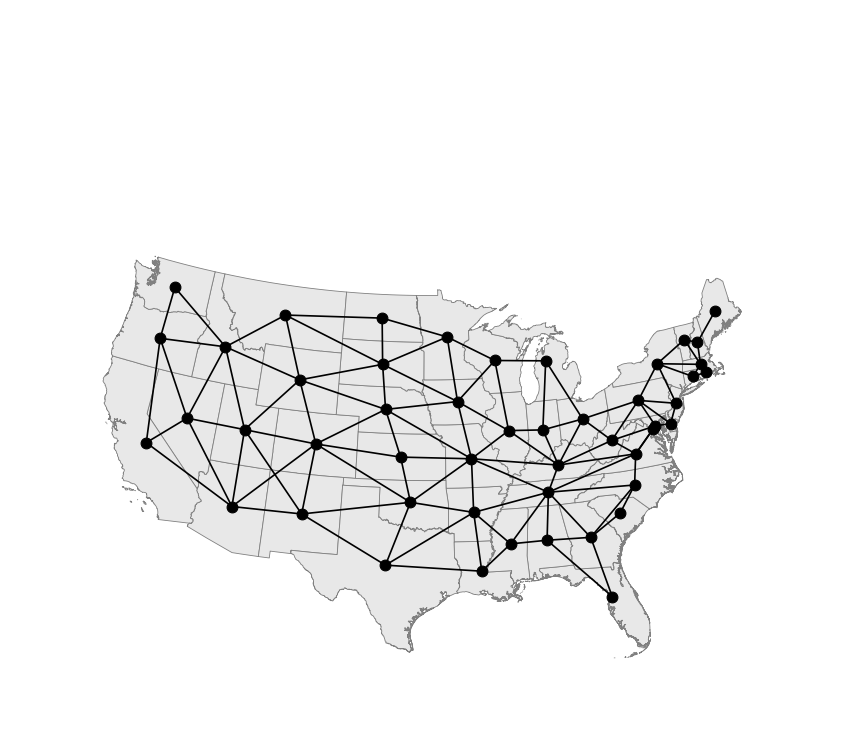
\includegraphics[width=\textwidth]{figures/dual_graph_a}
  \caption{Geographic units with dual graph $G$.}
  \label{fig:dual:a}
\end{subfigure}
\hfill
\begin{subfigure}[t]{0.32\textwidth}
  \centering
  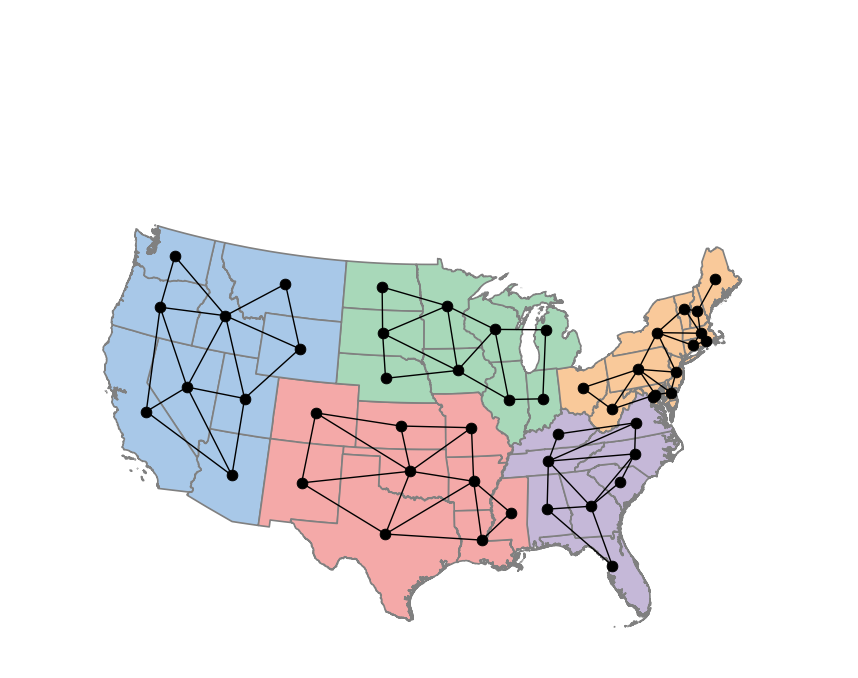
\includegraphics[width=\textwidth]{figures/dual_graph_b}
  \caption{A partition of $G^1$ into $k=6$ contiguous districts.}
  \label{fig:dual:b}
\end{subfigure}
\hfill
\begin{subfigure}[t]{0.32\textwidth}
  \centering
  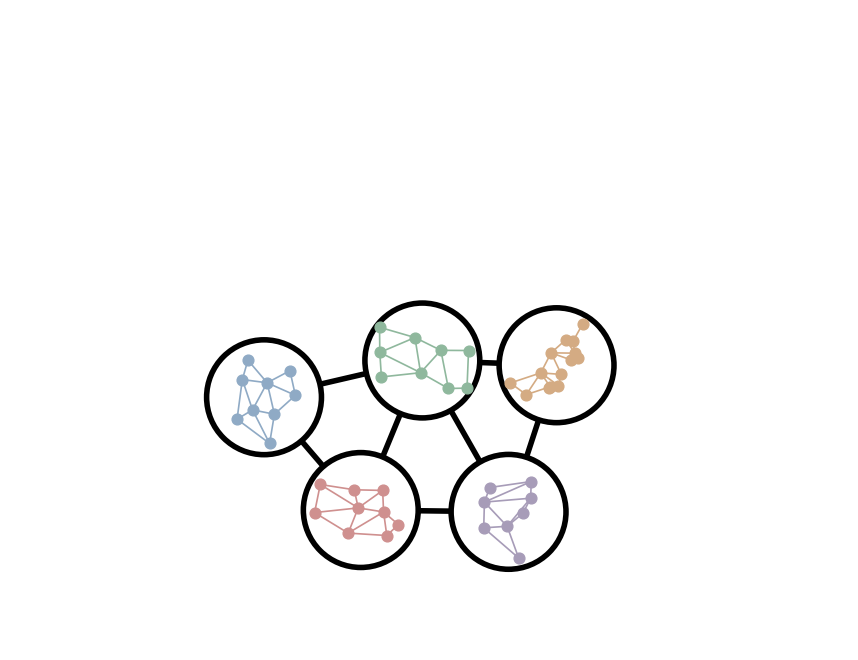
\includegraphics[width=\textwidth]{figures/dual_graph_c}
  \caption{Supergraph $G^{2}$. Each supernode represents a district.}
  \label{fig:dual:c}
\end{subfigure}
\caption{From geographic units to the supergraph used by FalCom.}
\label{fig:dual}
\end{figure}



\noindent with the convention $\mathcal{P}^0 = V^1$. The containment condition
in~\eqref{eq:hierarchy} ensures that every level-$\ell$ district is a union of
level-$(\ell{-}1)$ districts, which is the graph-theoretic counterpart of the
hierarchy constraint~\eqref{cons:hierarchy} in the MIP formulation.

At each level $\ell$, the partition $\mathcal{P}^\ell$ is equipped with two
functions. A \emph{facility assignment}
%
\[
    f^\ell \colon \mathcal{P}^\ell \to F^\ell
\]
%
maps each district to exactly one candidate facility site within it. A
\emph{capacity assignment}
%
\[
    c^\ell \colon \mathcal{P}^\ell \to \{c^{\ell}_{\min}, \ldots, c^{\ell}_{\max}\}
\]
%
specifies the number of service teams allocated to each district. At level $1$ the capacity is chosen by the chain. At level $\ell \geq 2$ it is the derived quantity $c^\ell(D) = \sum_{D' \in D} c^{\ell-1}(D')$, the aggregate capacity of the member districts, so the bounds $c^\ell_{\min} \leq c^\ell(D) \leq c^\ell_{\max}$ constrain the grouping rather than a separate decision.  In this paper, each district contains exactly one assigned facility, so $c^\ell(D_i^\ell)$ denotes both the district's capacity and that of its assigned facility.  In
other districting settings where multiple facilities may operate within a single district, $c^\ell(D_i^\ell)$ would represent the aggregate capacity of all assigned facilities in the district.  For convenience, we extend the capacity notation to arbitrary subgraphs: for a subgraph $H$ of $G^\ell$, we write
%
\[
    c_H \;=\; \sum_{D_i^\ell \subseteq H} c^\ell(D_i^\ell)
\]
%
for the \emph{aggregate capacity} of $H$, i.e., the total number of service teams allocated to the districts contained in~$H$.
Each base-level node $v \in V^1$ carries a non-negative \emph{demand}
$d_v \geq 0$, as introduced in Section~\ref{sec:model}. We use $d(v) \equiv d_v$ interchangeably and reserve the two-argument form $\mathrm{d}(\cdot, \cdot)$ for the travel distance metric used in Section~\ref{sec:facility}.
For higher levels $\ell \geq 2$, the demand of a supernode $v \in V^\ell$
is the aggregate demand of the base-level units it contains.
Extending this to subgraphs, for any
subgraph $H$ of $G^\ell$ we write
%
\[
    d_H \;=\; \sum_{v \in G^1[H]} d_v
\]
%
for the \emph{total demand} of the base-level units contained in~$H$.  When
$H$ is a subgraph of the base graph $G^1$, this reduces to
$d_H = \sum_{v \in V(H)} d_v$.  For individual districts and subtrees, we
use function notation $d(D_i^\ell)$ and $d_H$ to distinguish partition
elements from graphs.

We emphasize that the number of districts $k_\ell = |\mathcal{P}^\ell|$ is not fixed in advance:
it is determined jointly by the capacity constraint and the demand distribution.
Two solutions in $\Omega$ may have different numbers of districts at the same
level.

A \emph{solution} to the hierarchical capacitated facility location problem is a tuple
%
\begin{equation}\label{eq:solution}
    s = \bigl(\mathcal{P}^\ell,\, f^\ell,\, c^\ell
    \;\big|\; \ell \in L\bigr) \in \Omega,
\end{equation}
%
where $\Omega$ denotes the set of all such tuples.




%% --------------------------------------------------
\subsection{Constraint Rules and Feasibility}
\label{sec:rules}
%% --------------------------------------------------

The graph-partitioning framework automatically satisfies several constraints
from the MIP formulation in Section~\ref{sec:model}:
\medskip
%
\begin{itemize}[nosep]
  \item \textbf{Unique assignment}~\eqref{cons:assignment}: since
    $\mathcal{P}^\ell$ is a partition, every unit belongs to exactly one
    district.
  \item \textbf{Hierarchical containment}~\eqref{cons:hierarchy}: enforced by
    the nesting condition~\eqref{eq:hierarchy}.
  \item \textbf{Facility-capacity link}~\eqref{cons4}: the opening decision of a facility is tied to its capacity level by the definition of the assignment function $f^{\ell}$.
  \item \textbf{Integrality}~\eqref{cons:integrality}: the functions $f^\ell$
    and $c^\ell$ are integer-valued by construction.
\end{itemize}
\medskip
The remaining constraints require explicit enforcement. We collect them into a
rule set $\mathcal{C} = \bigcup_{\ell \in L} \mathcal{C}^\ell$, where
%
\begin{equation}\label{eq:rules}
    \mathcal{C}^\ell = \bigl\{
        \mathrm{contiguity}(\mathcal{P}^\ell),\;
        \mathrm{balance}(\mathcal{P}^\ell, c^\ell),\;
        \mathrm{coverage}(\mathcal{P}^\ell, c^\ell)
    \bigr\}.
\end{equation}
%
Each rule corresponds to a MIP constraint from Section~\ref{sec:model}:
\emph{contiguity} requires that every $G^\ell[D_i^\ell]$ is connected, corresponding to constraint~\eqref{cons:contiguity}. \emph{Balance} is a per-unit window at each level, stated as a property of the state. Let $\bar d = d/\lceil d/w\rceil$ be the demand per unit of capacity. Every superdistrict $D^2$ satisfies $(1{-}\varepsilon^2)\,\bar d\, c^2(D^2) \leq d(D^2) \leq (1{+}\varepsilon^2)\,\bar d\, c^2(D^2)$, and every level-1 district $D^1$ of capacity $c$ satisfies $(1{-}\varepsilon^2)\bigl(1 - \varepsilon^1\tfrac{c+1}{2c}\bigr)\, c\, \bar d \leq d(D^1) \leq (1{+}\varepsilon^2)\bigl(1 + \varepsilon^1\tfrac{c+1}{2c}\bigr)\, c\, \bar d$. The level-1 window is what the recursive partitioning of Section~\ref{sec:recursive} guarantees for every district it produces (Proposition~\ref{prop:effective}): at the time of the cut a district is held to a tighter window around the per-unit demand of the region being re-cut, and the two tolerances compound because that region is a superdistrict within its own level-2 window. The recursion produces only states that satisfy the rule; whether every state that satisfies it is reachable is open (Section~\ref{sec:convergence-status}). The rule corresponds to constraint~\eqref{cons:balance} with tolerance $\varepsilon^2$ at level $2$ and $(1{+}\varepsilon^1)(1{+}\varepsilon^2)-1$ at level $1$, with the windows centred at $\bar d$ in place of $w$; Section~\ref{sec:exp-milp} states how the two feasible sets differ on the instances it compares. \emph{Coverage} bounds the aggregate capacity, corresponding to constraint~\eqref{cons:coverage}; the sampler fixes the total capacity at the bound $\lceil d/w\rceil$ in its initial state and every proposal conserves it (Section~\ref{sec:outline}), so sampled states use full coverage. Three further rules are part of $\mathcal{C}$: every level-1 district contains a candidate site, which is the domain of $f^1$; every superdistrict contains at least $\kappa^2_{\min}$ districts, as in constraint~\eqref{cons:minL1perL2}; and every capacity lies in $[c^\ell_{\min}, c^\ell_{\max}]$, with $c^2$ the aggregate of the member capacities, as in constraints~\eqref{cons4} and~\eqref{cons:aggregate}. In FalCom, each rule in $\mathcal{C}^\ell$ is satisfied by a specific algorithmic phase we will discuss in Section~\ref{sec:falcom}.

A solution $s \in \Omega$ is \emph{feasible} if it satisfies every rule in
$\mathcal{C}$. The \emph{feasible state space} is
%
\begin{equation}\label{eq:feasible}
    \Omega_\mathcal{C} = \bigl\{ s \in \Omega :
    s \text{ satisfies all constraints in } \mathcal{C} \bigr\}.
\end{equation}
%
Each $s \in \Omega_\mathcal{C}$ is a \emph{state} of FalCom.

The partition $\mathcal{P}^\ell$ encodes the assignment variables $x_{ij}^\ell$,
the facility assignment $f^\ell$ encodes the opening variables $y_j^\ell$, and
the capacity function $c^\ell$ encodes $c^{\ell}_j$. A state $s \in \Omega_\mathcal{C}$ yields a feasible solution $(x_{ij}^\ell, y_j^\ell, c^{\ell}_j)$ of constraints~\eqref{cons:assignment}--\eqref{cons:integrality} once the balance windows of constraint~\eqref{cons:balance} are centred at $\bar d$ and widened to tolerance $(1{+}\varepsilon^1)(1{+}\varepsilon^2)-1$ at level $1$, provided that every superdistrict contains a level-2 candidate. Conversely, a feasible solution that uses the full coverage bound, keeps at least $\kappa^2_{\min}$ districts per superdistrict, places a candidate in every district and satisfies the balance rule of $\mathcal{C}$ corresponds to a state of $\Omega_\mathcal{C}$. Neither direction asserts that the chain reaches every such state.



%% -----------------------------------------------------------------------
\section{FalCom: A Sampling Method}
\label{sec:falcom}
%% -----------------------------------------------------------------------

FalCom carries the merge-and-split move of ReCom (Section~\ref{sec:literature}) from political redistricting to hierarchical capacitated facility location, generalizing it in two directions: (1)~a hierarchical two-level proposal that operates on a supergraph to localize computation, and (2)~a recursive partitioning scheme that produces a variable number of districts under capacity constraints, with a facility assigned to every district.

%% --------------------------------------------------
\subsection{Outline of FalCom}
\label{sec:outline}
%% --------------------------------------------------

The design of FalCom rests on two ideas. First, partitioning a graph by sampling a spanning tree and cutting an edge produces connected components by construction, so contiguity is never violated and never needs repair. Second, the supergraph $G^2$ selects \emph{which region} of the base graph to re-partition. Each iteration therefore touches a local subgraph rather than the full graph, and the level-1 part of a step costs in proportion to the selected superdistrict rather than to $|V^1|$, while the level-2 part re-partitions the supergraph of $k_1$ nodes.

FalCom consists of four phases: a \emph{hierarchical proposal} phase (Section~\ref{sec:proposal}), a \emph{recursive partitioning} phase (Section~\ref{sec:recursive}), a \emph{capacitated tree cut} phase (Section~\ref{sec:capacitated}), and a \emph{facility assignment} phase (Section~\ref{sec:facility}). We present the method for two levels ($|L| = 2$). The extension to $|L| > 2$ is immediate by induction on the levels of the hierarchy.

We write $G^2(\mathcal{P}^1)$ for the supergraph induced by a partition $\mathcal{P}^1$, as defined in Section~\ref{sec:statespace}. The chain is initialized with a feasible state $s^{(0)} \in \Omega_\mathcal{C}$ produced by the recursive partitioning phase, applied to the full base graph or zone by zone (see the initialization paragraph after Algorithm~\ref{alg:overview}). Each iteration $(i)$ produces a candidate next state for iteration $(i+1)$
%
\[
    s^{(i)} = \bigl(\mathcal{P}^\ell, f^\ell, c^\ell
    \;\big|\; \ell=1,2)^{(i)}
    \;\longmapsto\;
    s^{(i+1)} = \bigl(\mathcal{P}^\ell, f^\ell, c^\ell
    \;\big|\; \ell=1,2)^{(i+1)}
\]
%
\begin{figure}[t]
\centering

%% Color palette
\definecolor{super}{RGB}{100,100,100} 
\definecolor{colA}{RGB}{255,220,80}    % yellow  - D1
\definecolor{colB}{RGB}{130,200,130}   % green   - D2
\definecolor{colC}{RGB}{100,160,220}   % blue    - D3
\definecolor{colD}{RGB}{255,160,80}    % orange  - D4
\definecolor{colE}{RGB}{180,130,210}   % purple  - D5
\definecolor{colF}{RGB}{220,120,120}   % red     - D6
\definecolor{colG}{RGB}{160,210,200}   % teal    - D7 (bottom strip)
\definecolor{merged}{RGB}{210,210,210} % merged (gray)
\definecolor{treeedge}{RGB}{100,100,100}
\definecolor{cutedge}{RGB}{200,30,30}
\definecolor{newA}{RGB}{255,240,150}
\definecolor{newB}{RGB}{150,220,200}

%% ------------------------------------------------------------------
%% Helpers
%% ------------------------------------------------------------------
\newcommand{\gridnode}[3]{% x, y, color
  \node[circle, draw=black, fill=#3, inner sep=0pt, minimum size=8pt] at (#1,#2) {};
}

\newcommand{\facilitynode}[3]{% x, y, color  (facility candidate = thick border + star)
  \node[star, star points=6, draw=black, fill=#3, inner sep=0pt,
        minimum size=10pt, line width=1pt] at (#1,#2) {};
}


%% ==================================================================
%%  ReCom VERSION  – no hierarchy, no capacity, no facility stars
%%  4 panels arranged horizontally
%% ==================================================================
\scalebox{0.8}{
\begin{tikzpicture}[
  arrow/.style={-{Stealth[length=6pt]}, thick, gray!70},
  label/.style={font=\small\bfseries},
  every node/.style={font=\small}
]



\def\s{0.58}   % node spacing (cm)

%% ================================================================
%%  PANEL 1 – Current partition state
%% ================================================================
\begin{scope}[xshift=0cm]

  %% District fills – rows 0-3
  \fill[colA, opacity=0.35, rounded corners=2pt]
    (-0.22*\s, 2*\s-0.22*\s) rectangle (1*\s+0.22*\s, 3*\s+0.22*\s);
  \fill[colB, opacity=0.35, rounded corners=2pt]
    (2*\s-0.22*\s, 2*\s-0.22*\s) rectangle (3*\s+0.22*\s, 3*\s+0.22*\s);
  \fill[colC, opacity=0.35, rounded corners=2pt]
    (4*\s-0.22*\s, 2*\s-0.22*\s) rectangle (5*\s+0.22*\s, 3*\s+0.22*\s);
  \fill[colD, opacity=0.35, rounded corners=2pt]
    (-0.22*\s, 0*\s-0.22*\s) rectangle (1*\s+0.22*\s, 1*\s+0.22*\s);
  \fill[colE, opacity=0.35, rounded corners=2pt]
    (2*\s-0.22*\s, 0*\s-0.22*\s) rectangle (3*\s+0.22*\s, 1*\s+0.22*\s);
  \fill[colF, opacity=0.35, rounded corners=2pt]
    (4*\s-0.22*\s, 0*\s-0.22*\s) rectangle (5*\s+0.22*\s, 1*\s+0.22*\s);
  %% Bottom strip district
  \fill[colG, opacity=0.55, rounded corners=2pt]
    (-0.22*\s, -2*\s-0.22*\s) rectangle (5*\s+0.22*\s, -1*\s+0.22*\s);

%% Superdistrict 1 (cols 0-3, rows 0-3)
  \draw[super, ultra thick, rounded corners=3pt]
    (-0.35*\s, -0.35*\s) rectangle (3*\s+0.35*\s, 3*\s+0.35*\s);
  \node[font=\tiny\bfseries, text=super] at (1.5*\s, 3.2*\s+0.45) {\normalsize$D^2_1$};
  %% Superdistrict 2 (cols 0-3, rows 0-3)
  \draw[super, ultra thick, rounded corners=3pt]
    (3.65*\s, -0.35*\s) rectangle (5*\s+0.35*\s, 3*\s+0.35*\s);
  \node[font=\tiny\bfseries, text=super] at (4.6*\s, 3.2*\s+0.45) {\normalsize$D^2_2$};
  %% Superdistrict 3 (cols 0-3, rows 0-3)
  \draw[super, ultra thick, rounded corners=3pt]
    (-0.3*\s, -2.15*\s-0.22*\s) rectangle (5.1*\s+0.22*\s, -0.86*\s+0.22*\s);
  \node[font=\tiny\bfseries, text=super] at (-1*\s, -2.3*\s+0.45) {\normalsize$D^2_3$};

  
  
  %% Grid edges – rows 0-3
  \foreach \r in {0,1,2,3} {
    \foreach \c in {0,...,4} {
      \draw[gray!40, thin] (\c*\s, \r*\s) -- (\c*\s+\s, \r*\s);
    }
  }
  \foreach \c in {0,...,5} {
    \foreach \r in {0,1,2} {
      \draw[gray!40, thin] (\c*\s, \r*\s) -- (\c*\s, \r*\s+\s);
    }
  }
  %% Grid edges – bottom strip
  \foreach \r in {-2,-1} {
    \foreach \c in {0,...,4} {
      \draw[gray!40, thin] (\c*\s, \r*\s) -- (\c*\s+\s, \r*\s);
    }
  }
  \foreach \c in {0,...,5} {
    \draw[gray!40, thin] (\c*\s, -2*\s) -- (\c*\s, -1*\s);
    \draw[gray!40, thin] (\c*\s, -1*\s) -- (\c*\s, 0);
  }

  %% Nodes – rows 0-3
  \foreach \r in {2,3} {
    \gridnode{0*\s}{\r*\s}{colA}
    \gridnode{1*\s}{\r*\s}{colA}
    \gridnode{2*\s}{\r*\s}{colB}
    \gridnode{3*\s}{\r*\s}{colB}
    \gridnode{4*\s}{\r*\s}{colC}
    \gridnode{5*\s}{\r*\s}{colC}
  }
  \foreach \r in {0,1} {
    \gridnode{0*\s}{\r*\s}{colD}
    \gridnode{1*\s}{\r*\s}{colD}
    \gridnode{2*\s}{\r*\s}{colE}
    \gridnode{3*\s}{\r*\s}{colE}
    \gridnode{4*\s}{\r*\s}{colF}
    \gridnode{5*\s}{\r*\s}{colF}
  }
  %% Nodes – bottom strip
  \foreach \r in {-2,-1} {
    \foreach \c in {0,...,5} {
      \gridnode{\c*\s}{\r*\s}{colG}
    }
  }

%% Facility candidates (stars): one per district
  \facilitynode{0*\s}{3*\s}{colA}
  \facilitynode{2*\s}{2*\s}{colB}
  \facilitynode{5*\s}{3*\s}{colC}
  \facilitynode{1*\s}{0*\s}{colD}
  \facilitynode{3*\s}{1*\s}{colE}
  \facilitynode{4*\s}{0*\s}{colF}
  \facilitynode{2*\s}{-2*\s}{colG}

  
  \node[label] at (2.5*\s, -2*\s-0.7) {(1) Partition $V^{2}$};

\end{scope}

%% Arrow 1→2
\draw[arrow] (5*\s+0.45, 0.5*\s) -- +(0.45,0);

%% ================================================================
%%  PANEL 2 – Select merge pair (districts D1+D2 highlighted)
%% ================================================================
\begin{scope}[xshift=4.5cm]

  %% Unchanged districts (faded)
  \fill[colC, opacity=0.35, rounded corners=2pt]
    (4*\s-0.22*\s, 2*\s-0.22*\s) rectangle (5*\s+0.22*\s, 3*\s+0.22*\s);
  \fill[colF, opacity=0.35, rounded corners=2pt]
    (4*\s-0.22*\s, 0*\s-0.22*\s) rectangle (5*\s+0.22*\s, 1*\s+0.22*\s);
  \fill[colG, opacity=0.35, rounded corners=2pt]
    (-0.22*\s, -2*\s-0.22*\s) rectangle (5*\s+0.22*\s, -1*\s+0.22*\s);

  %% Merge region highlight (cols 0-3, rows 0-3)
  \fill[colA!30, opacity=0, rounded corners=3pt]
    (-0.35*\s, -0.35*\s) rectangle (3*\s+0.35*\s, 3*\s+0.35*\s);
  \draw[colA!60!colB, ultra thick, rounded corners=3pt]
    (-0.35*\s, -0.35*\s) rectangle (3*\s+0.35*\s, 3*\s+0.35*\s);
  \node[font=\tiny\bfseries, text=colA!60!colB] at (1.5*\s, 3*\s+0.5) {merged \normalsize $D^2_1$};

  %% Grid edges – rows 0-3
  \foreach \r in {0,1,2,3} {
    \foreach \c in {0,1,2,4} {
      \draw[gray!40, thin] (\c*\s, \r*\s) -- (\c*\s+\s, \r*\s);
    }
  }
  \foreach \c in {0,...,5} {
    \foreach \r in {0,1,2} {
      \draw[gray!40, thin] (\c*\s, \r*\s) -- (\c*\s, \r*\s+\s);
    }
  }
  %% Grid edges – bottom strip
  \foreach \r in {-2,-1} {
    \foreach \c in {0,...,4} {
      \draw[gray!40, thin] (\c*\s, \r*\s) -- (\c*\s+\s, \r*\s);
    }
  }
  \foreach \c in {0,...,5} {
    \foreach \r in {-2,1} {
      \draw[gray!40, thin] (\c*\s, \r*\s) -- (\c*\s, \r*\s+\s);
    }
  }
\foreach \c in {4,5} {
    \foreach \r in {-1,0} {
      \draw[gray!40, thin] (\c*\s, \r*\s) -- (\c*\s, \r*\s+\s);
    }
  }

  %% Nodes – merge region gray, right strip colored
  \foreach \r in {0,...,3} {
    \foreach \c in {0,...,3} {
      \gridnode{\c*\s}{\r*\s}{gray!55}
    }
  }
  \foreach \r in {2,3} {
    \gridnode{4*\s}{\r*\s}{colC}
    \gridnode{5*\s}{\r*\s}{colC}
  }
  \foreach \r in {0,1} {
    \gridnode{4*\s}{\r*\s}{colF}
    \gridnode{5*\s}{\r*\s}{colF}
  }
  \foreach \r in {-2,-1} {
    \foreach \c in {0,...,5} {
      \gridnode{\c*\s}{\r*\s}{colG}
    }
  }


% facility nodes
  \facilitynode{5*\s}{3*\s}{colC}
  \facilitynode{4*\s}{0*\s}{colF}
  \facilitynode{2*\s}{-2*\s}{colG}
  

  \node[label] at (2.5*\s, -2*\s-0.7) {(2) Merge superdistrict};
\end{scope}

%% Arrow 2→3
\draw[arrow] (4.5cm + 160*\s+0.45, 0.5*\s) -- +(0.45,0);

%% ================================================================
%%  PANEL 3 – Spanning tree + cut on merged region
%% ================================================================
\begin{scope}[xshift=9.0cm]

  %% Unchanged districts (right strip + bottom)
  \fill[colC, opacity=0.35, rounded corners=2pt]
    (4*\s-0.22*\s, 2*\s-0.22*\s) rectangle (5*\s+0.22*\s, 3*\s+0.22*\s);
  \fill[colF, opacity=0.35, rounded corners=2pt]
    (4*\s-0.22*\s, 0*\s-0.22*\s) rectangle (5*\s+0.22*\s, 1*\s+0.22*\s);
  \fill[colG, opacity=0.35, rounded corners=2pt]
    (-0.22*\s, -2*\s-0.22*\s) rectangle (5*\s+0.22*\s, -1*\s+0.22*\s);

  %% Spanning tree edges on the merged 4×4 block
  \draw[treeedge, very thick]
    (0,3*\s) -- (1*\s,3*\s) 
    (2*\s,3*\s) -- (3*\s,3*\s)
    (0,3*\s) -- (0,2*\s)
    (1*\s,3*\s) -- (1*\s,2*\s)
    (2*\s,3*\s) -- (2*\s,2*\s) 
    (3*\s,3*\s) -- (3*\s,2*\s) -- (3*\s,1*\s) -- (3*\s,0)
    (0,2*\s) -- (0,1*\s) -- (0,0)
    (1*\s,2*\s) -- (1*\s,1*\s)
    (2*\s,1*\s) -- (2*\s,0)
    (1*\s,0) -- (1*\s,1*\s)
    (2*\s,0) -- (3*\s,0);
  %% Cut edge (red)
  \draw[cutedge, very thick, line cap=round] (1*\s,1*\s) -- (2*\s,1*\s);
  \node[font=\tiny, text=cutedge] at (1.5*\s, 0.8*\s+0.38) {Cut};


  \foreach \c in {4,5} {
    \foreach \r in {0,1,2} {
      \draw[gray!40, thin] (\c*\s, \r*\s) -- (\c*\s, \r*\s+\s);
    }
  }
  %% Grid edges – bottom strip
  \foreach \r in {-2,-1} {
    \foreach \c in {0,...,4} {
      \draw[gray!40, thin] (\c*\s, \r*\s) -- (\c*\s+\s, \r*\s);
    }
  }
  \foreach \c in {4,5} {
    \draw[gray!40, thin] (\c*\s, -2*\s) -- (\c*\s, -1*\s);
    \draw[gray!40, thin] (\c*\s, -1*\s) -- (\c*\s, 0);
  }

  %% Nodes
  \foreach \r in {0,...,3} {
    \foreach \c in {0,...,3} {
      \gridnode{\c*\s}{\r*\s}{gray!55}
    }
  }
  \foreach \r in {2,3} {
    \gridnode{4*\s}{\r*\s}{colC}
    \gridnode{5*\s}{\r*\s}{colC}
  }
  \foreach \r in {0,1} {
    \gridnode{4*\s}{\r*\s}{colF}
    \gridnode{5*\s}{\r*\s}{colF}
  }
  \foreach \r in {-2,-1} {
    \foreach \c in {0,...,5} {
      \gridnode{\c*\s}{\r*\s}{colG}
    }
  }

  \facilitynode{5*\s}{3*\s}{colC}
  \facilitynode{4*\s}{0*\s}{colF}
  \facilitynode{2*\s}{-2*\s}{colG}

  \node[label] at (2.5*\s, -2*\s-0.7) {(3) Cut spanning tree};
\end{scope}

%% Arrow 3→4
\draw[arrow] (9.0cm + 160*\s+0.45, 0.5*\s) -- +(0.45,0);

%% ================================================================
%%  PANEL 4 – New partition state
%% ================================================================
\begin{scope}[xshift=13.5cm]

  %% New districts from cut (cols 0-1 → newA, cols 2-3 → colD, full rows 0-3)
  \fill[newA, opacity=0.35, rounded corners=2pt]
    (-0.22*\s, -0.22*\s) rectangle (1*\s+0.22*\s, 3*\s+0.22*\s);
  \fill[colD, opacity=0.35, rounded corners=2pt]
    (2*\s-0.22*\s, -0.22*\s) rectangle (3*\s+0.22*\s, 3*\s+0.22*\s);

  %% Unchanged right strip + bottom
  \fill[colC, opacity=0.35, rounded corners=2pt]
    (4*\s-0.22*\s, 2*\s-0.22*\s) rectangle (5*\s+0.22*\s, 3*\s+0.22*\s);
  \fill[colF, opacity=0.35, rounded corners=2pt]
    (4*\s-0.22*\s, 0*\s-0.22*\s) rectangle (5*\s+0.22*\s, 1*\s+0.22*\s);
  \fill[colG, opacity=0.35, rounded corners=2pt]
    (-0.22*\s, -2*\s-0.22*\s) rectangle (5*\s+0.22*\s, -1*\s+0.22*\s);

  %% Grid edges – rows 0-3
  \foreach \r in {0,1,2,3} {
    \foreach \c in {0,...,4} {
      \draw[gray!40, thin] (\c*\s, \r*\s) -- (\c*\s+\s, \r*\s);
    }
  }
  \foreach \c in {0,...,5} {
    \foreach \r in {0,1,2} {
      \draw[gray!40, thin] (\c*\s, \r*\s) -- (\c*\s, \r*\s+\s);
    }
  }
  %% Grid edges – bottom strip
  \foreach \r in {-2,-1} {
    \foreach \c in {0,...,4} {
      \draw[gray!40, thin] (\c*\s, \r*\s) -- (\c*\s+\s, \r*\s);
    }
  }
  \foreach \c in {0,...,5} {
    \draw[gray!40, thin] (\c*\s, -2*\s) -- (\c*\s, -1*\s);
    \draw[gray!40, thin] (\c*\s, -1*\s) -- (\c*\s, 0);
  }

  %% Nodes
  \foreach \r in {0,...,3} {
    \gridnode{0*\s}{\r*\s}{newA}
    \gridnode{1*\s}{\r*\s}{newA}
    \gridnode{2*\s}{\r*\s}{colD}
    \gridnode{3*\s}{\r*\s}{colD}
  }
  \foreach \r in {2,3} {
    \gridnode{4*\s}{\r*\s}{colC}
    \gridnode{5*\s}{\r*\s}{colC}
  }
  \foreach \r in {0,1} {
    \gridnode{4*\s}{\r*\s}{colF}
    \gridnode{5*\s}{\r*\s}{colF}
  }
  \foreach \r in {-2,-1} {
    \foreach \c in {0,...,5} {
      \gridnode{\c*\s}{\r*\s}{colG}
    }
  }

%% New facility candidates (stars)
  \facilitynode{0*\s}{3*\s}{newA}
  \facilitynode{2*\s}{3*\s}{colD}
  \facilitynode{1*\s}{0*\s}{newA}
  \facilitynode{3*\s}{0*\s}{colD}
  \facilitynode{5*\s}{3*\s}{colC}
  \facilitynode{4*\s}{0*\s}{colF}
  \facilitynode{2*\s}{-2*\s}{colG}
  
  \node[label] at (2.5*\s, -2*\s-0.7) {(4) 5 new districts};
\end{scope}

%% ================================================================
%%  LEGEND
%% ================================================================
\begin{scope}[xshift=0cm, yshift=-2.4cm]

\end{scope}


  
\end{tikzpicture}
}
\caption{One iteration of FalCom: (1)~Partition supergraph;
         (2)~Merge a superdistrict;
         (3)~a spanning tree is built on the merged region and a feasible
         cut edge is sampled;
         (4)~the resulting new state $s_{i+1}$. Star-nodes indicate candidate facilities.}
\label{fig:bottom}
\end{figure}

%
via the following inter-level strategy:
%
\medskip

\begin{enumerate}[nosep]
    \item \textbf{Upper level.} Build the supergraph
        $G^2\bigl((\mathcal{P}^1)^{(i)}\bigr)$ and partition it into new
        superdistricts $(\mathcal{P}^2)^{(i+1)}$ with capacity assignment
        $(c^2)^{(i+1)}$.
    \item \textbf{Lower level.} Choose one superdistrict
        $D^2 \in (\mathcal{P}^2)^{(i+1)}$ uniformly at random.
        Re-partition the induced subgraph $G^1[D^2]$ into new
        districts $D_1^1, \ldots, D_m^1$ with capacity assignment
        $(c^1)^{(i+1)}$, while keeping all districts outside $D^2$
        unchanged.
    \item \textbf{Facility assignment.} Assign $(f^1)^{(i+1)}$ and
        $(f^2)^{(i+1)}$ independently of the current state~$s^{(i)}$.
        \item \textbf{Accept/reject.} If every phase closed, i.e.\ every cut used in the proposal was admissible, accept $s^{(i+1)} \leftarrow s'$. Otherwise reject and set
        $s^{(i+1)} \leftarrow s^{(i)}$.
\end{enumerate}
\medskip

Steps~1 and~2 together constitute the \emph{hierarchical proposal phase}
(Section~\ref{sec:proposal}), which orchestrates the inter-level
interaction: it constructs the input tuple
$(H, c_H, \bar{d}_H, \varepsilon^\ell)$ that the recursive partitioning
phase requires, and chooses the demand target that anchors local
balance. Each step then invokes the recursive partitioning phase
(Section~\ref{sec:recursive}), which in turn calls the capacitated tree
cut phase (Section~\ref{sec:capacitated}) as a subroutine. In step~1,
solving for $(\mathcal{P}^2)^{(i+1)}, (c^2)^{(i+1)}$ amounts to
partitioning the supergraph $G^2\bigl((\mathcal{P}^1)^{(i)}\bigr)$ with
a feasible capacity assignment, using the global average demand per team
$\bar{d}$. In step~2, the same phase is invoked on the induced subgraph
$G^1[D^2]$ of the selected superdistrict with a \emph{local} demand
target $\bar{d}_H = d_H / c_H$, which Section~\ref{sec:proposal}
motivates as necessary whenever supergraph density deviates from the
global average. Step~3 assigns facilities as a deterministic function of the new partition (Section~\ref{sec:facility}), so every facility readout is a function of the state. Figure~\ref{fig:bottom}
illustrates one iteration of the inter-level strategy.


\medskip

\noindent\textbf{Acceptance rule.}\quad
After constructing the candidate state $s'$, FalCom accepts or rejects it.
All rules in $\mathcal{C}$ are satisfied by construction during the proposal
phases: contiguity by the spanning tree structure, capacity-demand balance
by the feasibility score $\phi$ defined in Section~\ref{sec:capacitated},
and total capacity-demand coverage by the recursive partitioning phase.
A proposal is accepted if all phases complete successfully. Otherwise the
chain remains at the current state $s^{(i)}$ and a new proposal is generated
in the next iteration.

Algorithm~\ref{alg:overview} summarizes one iteration.

\medskip

\begin{algorithm}[H]
\LinesNumbered
\caption{Outline of FalCom for $|L| = 2$}\label{alg:overview}

\KwIn{Base graph $G^1$; current state $s^{(i)} = (\mathcal{P}^\ell, f^\ell, c^\ell \mid \ell=1,2)^{(i)}$; parameters $w$, $\varepsilon^\ell$, $c^\ell_{\min}$, $c^\ell_{\max}$, $\kappa^2_{\min}$}
\KwOut{Next state $s^{(i+1)}$}

\BlankLine

$G^2 \leftarrow G^2\bigl((\mathcal{P}^1)^{(i)}\bigr)$ \tcp*{supergraph of the current level-1 partition}
Partition $G^2$ into superdistricts $(\mathcal{P}^2)^{(i+1)}$ with $(c^2)^{(i+1)}$ \tcp*{Sections~\ref{sec:recursive},~\ref{sec:capacitated}}
Choose superdistrict $D^2 \in (\mathcal{P}^2)^{(i+1)}$
    uniformly at random\;

$\mathcal{P} \leftarrow (\mathcal{P}^1)^{(i)}
    \setminus \{D \in (\mathcal{P}^1)^{(i)} : D \subseteq D^2\}$
    \tcp*{preserve unchanged districts}

Partition $G^1[D^2]$ into districts
    $D_1^1, \ldots, D_m^1$ with $(c^1)^{(i+1)}$
    \tcp*{Sections~\ref{sec:recursive},~\ref{sec:capacitated}}
\lIf{$m < \kappa^2_{\min}$}{\Return{$s^{(i)}$}}

$(\mathcal{P}^1)^{(i+1)} \leftarrow
    \mathcal{P} \cup \{D_1^1, \ldots, D_m^1\}$\;

Assign facilities $(f^1)^{(i+1)} \colon (\mathcal{P}^1)^{(i+1)} \to F^1$ and $(f^2)^{(i+1)} \colon (\mathcal{P}^2)^{(i+1)} \to F^2$ \tcp*{Section~\ref{sec:facility}}
$s' \leftarrow
    (\mathcal{P}^\ell, f^\ell, c^\ell \mid \ell=1,2)^{(i+1)}$\;

\BlankLine
\uIf{every phase closed
     \tcp*{Section~\ref{sec:capacitated}}}{
    $s^{(i+1)} \leftarrow s'$\;
}
\Else{
    $s^{(i+1)} \leftarrow s^{(i)}$ \tcp*{reject: stay at current state}
}
\Return{$s^{(i+1)}$}
\end{algorithm}

\medskip

\paragraph{Initialization.} Our implementation therefore constructs a feasible initial state by applying the recursive partitioning phase
described in Section~\ref{sec:recursive} directly to the full base graph~$G^1$. Given the total demand $d_{G^1}$ and the maximum per-team workload~$w$, the number of teams or the total capacity $c_G$ equivalently is
set to $c_{G^1} = \lceil d_{G^1} / w \rceil$, and Algorithm~\ref{alg:recursive} is called with the inputs $(G^1, c_{G^1}, \bar{d}, \varepsilon^1)$ to recursively partition the graph $G^1$ yielding an initial partition $(\mathcal{P}^1)^{(0)}$ together with a
capacity assignment $(c^1)^{(0)}$ for a given $\varepsilon^1$. The supergraph $G^2\bigl((\mathcal{P}^1)^{(0)}\bigr)$ is then built, and a second call to \textit{RecursivePartitioning} on~$G^2$ yields the initial superdistrict partition $(\mathcal{P}^2)^{(0)}$ with $(c^2)^{(0)}$.  Facility assignments are computed deterministically via Equation~\eqref{eq:facility-assign}. The resulting initial state $s^{(0)} \in \Omega_\mathcal{C}$ is feasible by construction, and the chain begins producing valid samples immediately.

%% --------------------------------------------------
\subsection{Hierarchical Proposal Phase}
\label{sec:proposal}
%% --------------------------------------------------

As outlined in Section~\ref{sec:outline}, the supergraph is partitioned at every state of the chain, and FalCom re-designs the districts within one of the resulting superdistricts.  Both processes are carried out by the recursive partitioning phase in Section~\ref{sec:recursive}.  The hierarchical proposal phase manages the interaction between the two levels. At every state, it constructs the input tuple that the recursive partitioning phase requires and ensures that the capacity assignments are
consistent across levels.

The recursive partitioning phase takes the input
$(H,\; c_H,\; \bar{d}_H,\; \varepsilon^\ell)$, where $H$ is the connected subgraph to be partitioned, $c_H$ is its aggregate capacity (one unit per service team to allocate), $\bar{d}_H$ is the local demand target per team, and $\varepsilon^{\ell}$ is the balance tolerance at level $\ell$. The hierarchical proposal phase constructs this tuple differently for the upper and lower levels. Let $\bar{d} = d_{G^1} / c_{G^1}$ denote the \emph{global} average demand per team, where $c_{G^1} = \lceil d_{G^1} / w \rceil$ is the total number of service teams fixed by the coverage rule.

\medskip
\noindent\textbf{Upper level: Solve for $(\mathcal{P}^2)^{(i+1)},\;
(c^2)^{(i+1)}$ using $(\mathcal{P}^1)^{(i)}$.}\quad
We first construct the supergraph $G^2\bigl((\mathcal{P}^1)^{(i)}\bigr)$.
The total capacity at level~$2$ is the sum of the level-$1$ capacities,
$c_{G^2} = \sum_i c^1(D_i^1)$. Each superdistrict's capacity is the sum of its members' capacities, $c^2(S) = \sum_{D \subseteq S} c^1(D)$: it is not chosen from a window but given by the grouping, and the supergraph recursion admits a subtree when its aggregate capacity lies in $[c^2_{\min}, c^2_{\max}]$ and its demand within $(1 \pm \varepsilon^2)$ of that capacity times $\bar d$, with no debt term (Section~\ref{sec:capacitated}).  We pass the
input tuple $(G^2,\; c_{G^2},\; \bar{d},\; \varepsilon^2)$ to the recursive
partitioning phase, which partitions the supergraph into new superdistricts
$(\mathcal{P}^2)^{(i+1)} = \{D_1^2, D_2^2, \ldots, D_k^2\}$ with capacity
assignment $(c^2)^{(i+1)}$.  Here $\bar{d} = d/c_{G^2}$ is the global demand per unit of capacity, since the supergraph represents the entire region.

\medskip
\noindent\textbf{Lower level: Solve for $(\mathcal{P}^1)^{(i+1)},\;
(c^1)^{(i+1)}$ using $(\mathcal{P}^2)^{(i+1)}$.}\quad
After the upper level is settled, one superdistrict
$D^2 \in (\mathcal{P}^2)^{(i+1)}$ is selected uniformly at random.  Let
$H = G^1[D^2]$ be the subgraph of $G^1$ induced by the base-level units in
this superdistrict.  The total capacity to allocate in $H$ is
$c_H = c^2(D^2)$, and we compute a \emph{local} average demand per team
$\bar{d}_H = d_H / c_H$.  We then pass the input tuple
$(H,\; c_H,\; \bar{d}_H,\; \varepsilon^1)$ to the recursive partitioning
phase.

A local average is necessary because the demand density within the selected superdistrict may differ substantially from the global density. Using the global target $\bar{d}$ would systematically over- or under-allocate teams in dense or sparse regions. Section~\ref{sec:recursive} explains this in more detail.

Algorithm~\ref{alg:proposal} summarizes the hierarchical proposal phase.

\medskip
\medskip

\begin{algorithm}[H]
\LinesNumbered
\caption{Hierarchical proposal}\label{alg:proposal}
\KwIn{Current level-1 partition $\mathcal{P}^1$ with capacities $c^1$; global unit $\bar d$; tolerances $\varepsilon^1, \varepsilon^2$; capacity bounds; $\kappa^2_{\min}$}
\KwOut{$\mathcal{P}^1,\; \mathcal{P}^2,\; c^1,\; c^2$}

\BlankLine
\tcp{Upper level: supergraph partition}

$c_{G^2} \leftarrow \sum_{D_i^1 \in \mathcal{P}^1} c^1(D_i^1)$\;

$\mathcal{P}^2,\; c^2 \leftarrow
    \textit{RecursivePartitioning}\bigl(G^2,\; c_{G^2},\;
    \bar{d},\; \varepsilon^2\bigr)$ \tcp*{Section~\ref{sec:recursive}}
\lIf{the call returned Rejection}{\Return{Rejection}}

Select superdistrict $D^2 \in \mathcal{P}^2$ uniformly at random\;

\BlankLine
\tcp{Lower level: re-split selected superdistrict}

$H \leftarrow G^1[D^2]$\;

$c_H \leftarrow c^2(D^2)$, \quad $\bar{d}_H \leftarrow d_H \,/\, c_H$\;

$\mathcal{P}_H,\; c^1_H \leftarrow \textit{RecursivePartitioning}\bigl(H,\; c_H,\; \bar{d}_H,\; \varepsilon^1\bigr)$ \tcp*{Section~\ref{sec:recursive}}
\lIf{the call returned Rejection or $|\mathcal{P}_H| < \kappa^2_{\min}$}{\Return{Rejection}}
$\mathcal{P}^1 \leftarrow \bigl(\mathcal{P}^1 \setminus \{D \in \mathcal{P}^1 : D \subseteq D^2\}\bigr) \cup \mathcal{P}_H$, and $c^1$ likewise\;

\Return{$\mathcal{P}^1,\; \mathcal{P}^2,\; c^1,\; c^2$}
\end{algorithm}
\medskip
\medskip

The proposal reads only $(\mathcal{P}^1, c^1)$ of the current state: the level-2 partition, the capacities $c^2$ and the facilities are recomputed, so FalCom is a Markov chain on $(\mathcal{P}^1, c^1)$ whose level-2 component is a fresh draw of the supergraph recursion given $\mathcal{P}^1$, and the level-2 readouts of Section~\ref{sec:exp-emergency} are readouts of that conditional law. The new level-2 partition is a valid partition of the new supergraph because the re-cut superdistrict keeps its footprint and its new districts partition it. The key insight is that $\bar{d}_H$ is recomputed locally for the selected superdistrict at the lower level.  This allows the lower-level split to adapt
to the demand density of the specific region being re-partitioned, rather than
using the global workload target~$\bar{d}$.

The two-task structure above is one specific inter-level design: the upper
level is re-partitioned at every iteration, and the lower level adapts its
workload target to the resulting superdistricts.  Other designs are possible
depending on the application.  For instance, in problems where upper-level
boundaries are administratively fixed (e.g., existing precinct boundaries in
police zone design), the supergraph partition can be held constant and only the
lower-level re-split is performed.  Similarly, the capacity transfer rule,
how superdistrict capacity $c^2(D^2)$ constrains the lower-level split,
can be relaxed or tightened depending on whether the application requires
strict nesting or allows flexibility across levels.  We adopt the fully dynamic design because it provides the most general exploration of the state space. A systematic comparison of alternative inter-level designs is left to a follow-up study.

%% --------------------------------------------------
\subsection{Recursive Partitioning Phase}
\label{sec:recursive}
%% --------------------------------------------------

The recursive partitioning phase takes the input $(H,\; c_H,\; \bar{d}_H,\; \varepsilon^{\ell})$ constructed by the hierarchical proposal phase in Section~\ref{sec:proposal}, and divides $H$ into a collection of contiguous, capacity-demand balanced connected subgraphs of $H$, each carrying a capacity level and containing at least one facility candidate. The phase is called by both tasks of the hierarchical proposal, once on the supergraph $H=G^2$ to produce superdistricts, and once on a base-level subgraph $H \subset G^1$ to produce districts.

The phase works by repeatedly extracting one district at a time from a shrinking residual graph, using the capacitated tree cut phase detailed in Section~\ref{sec:capacitated}, until the entire graph is partitioned. Each extracted district $D_r$ must satisfy the \emph{global balance rule} $\mathrm{balance}(\mathcal{P}^\ell, c^\ell) \in \mathcal{C}^\ell$ given by
%
\begin{align}\label{eq:globalbalance}
    d(D_r) \in I
    :=& \bigl[\, (1 - \varepsilon^{\ell}) c^{\ell}(D_r)\,\bar{d}, \;\;
                      (1 + \varepsilon^{\ell}) c^{\ell}(D_r)\,\bar{d} \,\bigr] \\[4pt]
    =& \bigl[ c^{\ell}(D_r)\,\bar{d} - c^{\ell}(D_r)\,\tau^\ell,\; c^{\ell}(D_r)\,\bar{d} + c^{\ell}(D_r)\,\tau^\ell  \bigr]
\end{align}
%
\begingroup\sloppy
defined in Section \ref{sec:rules}, where $\tau^\ell = \varepsilon^{\ell}\,\bar{d}$ is the \emph{per-team tolerance}. The \emph{global coverage rule} $\mathrm{coverage}(\mathcal{P}^\ell, c^\ell)$ in $\mathcal{C}^{\ell}$ requires a \emph{local coverage rule}
%
\begin{equation}\label{eq:localcoverage}
\sum_{r=1}^{k} c^{\ell}(D_r) = c_H.
\end{equation}
%
The sequential extraction produces districts whose demands deviate from $\bar{d}_H$, and these deviations accumulate during the recursion. To ensure that the cumulative deviation does not violate the global balance and coverage rules for later districts, we design a debt-tracking mechanism and define local constraints accordingly. Without correction, the residual at the end of the recursion may carry a leftover demand that cannot simultaneously absorb the remaining capacity and respect~(\ref{eq:globalbalance}).
\endgroup

\paragraph{Recursion and residual graph.} Let $H^{(0)} := H$ be the initial graph of the recursion at the hierarchical level $\ell=1,2$. At each step $r \geq 1$, we extract a district $D_r$ from the previous residual graph $H^{(r-1)}$, yielding the current residual
%
\[
    H^{(r)} := H^{(r-1)} \setminus D_{r},
\]
%
where $H^{(r-1)} \setminus D_r$ denotes the subgraph of $H^{(r-1)}$ induced by $V_{H^{(r-1)}} \setminus D_r$. The process terminates after $k$ recursion steps when the remaining capacity reaches zero, producing the sequence of residual graphs
%
\[
    H^{(0)} \supset H^{(1)} \supset \cdots \supset H^{(k)}  = \emptyset,
\]
%
where inclusion denotes induced subgraph containment. The resulting partition of $V_H$ is $\mathcal{P}^{\ell}_H = \{D_1, \ldots, D_k\}$, where $V_H = \bigsqcup_{r=1}^{k} D_r$ with $D_r \neq \emptyset$ for all $r$, and each $D_r$ induces a connected subgraph of $H^{(r-1)}$. A capacity level $c^{\ell}(D_r) \in [c_{\min}^{\ell}, c_{\max}^{\ell}]$ is assigned to each district $D_r$ at the moment of its extraction, and the remaining capacity $c_{H^{(r)}}$ of the residual graph $H^{(r)}$ is updated by 
%
\begin{equation}\label{eq:capacityupdate}
    c_{H^{(0)}} = c_H, \quad c_{H^{(r)}} = c_{H^{(r-1)}} - c^\ell(D_r).
\end{equation}
%
as shown in Figure~\ref{fig:recursive}. Since each step consumes at least $c_{\min}^\ell \geq 1$ units of capacity, the recursion terminates in $k \leq c_H$ steps, when $c_{H^{(r)}}$ reaches zero, and the local coverage rule~(\ref{eq:localcoverage}) holds by construction. The number of districts $k$ is therefore determined endogenously by the recursion, not fixed a priori. We next introduce the debt mechanism and show how we control demand deviations to preserve the global balance rule~(\ref{eq:globalbalance}).


%% =====================================================================
%%  Figure: Recursive Partitioning (sequential district extraction)
%% =====================================================================

%% Color palette
\definecolor{distA}{RGB}{255,200,80}
\definecolor{distB}{RGB}{130,200,130}
\definecolor{distC}{RGB}{100,160,220}
\definecolor{distD}{RGB}{180,130,210}
\definecolor{residual}{RGB}{220,220,220}
\definecolor{treecol}{RGB}{80,80,80}
\definecolor{cutcol}{RGB}{200,30,30}
\definecolor{candcol}{RGB}{200,30,30}
\definecolor{feasible}{RGB}{40,160,40}
\definecolor{infeasible}{RGB}{180,180,180}

\newcommand{\gnode}[3]{% x, y, color
  \node[circle, draw=black!70, fill=#3, inner sep=0pt, minimum size=7pt] at (#1,#2) {};
}
\newcommand{\cand}[2]{% x, y  — candidate facility marker
  \node[star, star points=5, star point ratio=2.2, fill=candcol,
        inner sep=0pt, minimum size=5pt, draw=none] at (#1,#2) {};
}

\begin{figure}[t]
\centering
\scalebox{1.3}{
\begin{tikzpicture}[
  arrow/.style={-{Stealth[length=5pt]}, thick, gray!70},
  lbl/.style={font=\scriptsize\bfseries},
  every node/.style={font=\scriptsize}
]
\def\s{0.55}

%% --- Panel (a): Initial graph H^{(0)} with n=8 teams ---
\begin{scope}[xshift=0cm]
  \fill[residual, opacity=0.35, rounded corners=2pt]
    (-0.3*\s,-0.3*\s) rectangle (3*\s+0.3*\s, 3*\s+0.3*\s);

  %% Grid edges
  \foreach \r in {0,...,3} {
    \foreach \c in {0,...,2} {
      \draw[gray!40, thin] (\c*\s,\r*\s) -- (\c*\s+\s,\r*\s);
    }}
  \foreach \c in {0,...,3} {
    \foreach \r in {0,...,2} {
      \draw[gray!40, thin] (\c*\s,\r*\s) -- (\c*\s,\r*\s+\s);
    }}

  %% Nodes
  \foreach \r in {0,...,3} {
    \foreach \c in {0,...,3} {
      \gnode{\c*\s}{\r*\s}{residual}
    }}

  %% Candidates
  \cand{1*\s}{3*\s}  \cand{3*\s}{2*\s}
  \cand{0*\s}{0*\s}  \cand{2*\s}{1*\s}

  \node[lbl] at (1.5*\s, -0.5) {$c_{H^{(0)}}=8$};
\end{scope}

\draw[arrow] (2.8*\s+0.5, 1.5*\s) -- +(0.4,0);


%% --- Panel (b): Extract D_0, residual H^{(1)} ---
\begin{scope}[xshift=2.8cm]
  %% D_0 extracted (top-right)
  \fill[distA, opacity=0.35, rounded corners=2pt]
    (2*\s-0.25*\s, 2*\s-0.25*\s) rectangle (3*\s+0.25*\s, 3*\s+0.25*\s);

  %% Residual
  \fill[residual, opacity=0.35, rounded corners=2pt]
    (-0.3*\s,-0.3*\s) rectangle (3*\s+0.3*\s, 1*\s+0.3*\s);
  \fill[residual, opacity=0.35, rounded corners=2pt]
    (-0.3*\s, 1*\s-0.3*\s) rectangle (1*\s+0.3*\s, 3*\s+0.3*\s);

  %% Edges
  \foreach \r in {0,...,3} {
    \foreach \c in {0,...,2} {
      \draw[gray!40, thin] (\c*\s,\r*\s) -- (\c*\s+\s,\r*\s);
    }}
  \foreach \c in {0,...,3} {
    \foreach \r in {0,...,2} {
      \draw[gray!40, thin] (\c*\s,\r*\s) -- (\c*\s,\r*\s+\s);
    }}

  %% Nodes
  \foreach \r in {2,3} {
    \foreach \c in {2,3} {
      \gnode{\c*\s}{\r*\s}{distA}
    }}
  \foreach \r in {0,1} {
    \foreach \c in {0,...,3} {
      \gnode{\c*\s}{\r*\s}{residual}
    }}
  \foreach \r in {2,3} {
    \foreach \c in {0,1} {
      \gnode{\c*\s}{\r*\s}{residual}
    }}

  \cand{1*\s}{3*\s}  \cand{3*\s}{2*\s}
  \cand{0*\s}{0*\s}  \cand{2*\s}{1*\s}

  \node[font=\tiny, distA!70!black] at (2.5*\s, 3*\s+0.35) {$c^{\ell}(D_1){=}2$};
  \node[lbl] at (1.5*\s, -0.5) {$c_{H^{(1)}}=6$};
\end{scope}

\draw[arrow] (4.75cm + 3*\s+0.5, 1.5*\s) -- +(0.4,0);

%% --- Panel (c): Extract D_1, residual H^{(2)} ---
\begin{scope}[xshift=5.6cm]
  %% D_0
  \fill[distA, opacity=0.35, rounded corners=2pt]
    (2*\s-0.25*\s, 2*\s-0.25*\s) rectangle (3*\s+0.25*\s, 3*\s+0.25*\s);
  %% D_1
  \fill[distB, opacity=0.35, rounded corners=2pt]
    (-0.25*\s, 2*\s-0.25*\s) rectangle (1*\s+0.25*\s, 3*\s+0.25*\s);

  %% Residual
  \fill[residual, opacity=0.35, rounded corners=2pt]
    (-0.3*\s,-0.3*\s) rectangle (3*\s+0.3*\s, 1*\s+0.3*\s);

  \foreach \r in {0,...,3} {
    \foreach \c in {0,...,2} {
      \draw[gray!40, thin] (\c*\s,\r*\s) -- (\c*\s+\s,\r*\s);
    }}
  \foreach \c in {0,...,3} {
    \foreach \r in {0,...,2} {
      \draw[gray!40, thin] (\c*\s,\r*\s) -- (\c*\s,\r*\s+\s);
    }}

  \foreach \r in {2,3} {
    \gnode{2*\s}{\r*\s}{distA}  \gnode{3*\s}{\r*\s}{distA}
    \gnode{0*\s}{\r*\s}{distB}  \gnode{1*\s}{\r*\s}{distB}
  }
  \foreach \r in {0,1} {
    \foreach \c in {0,...,3} {
      \gnode{\c*\s}{\r*\s}{residual}
    }}

  \cand{1*\s}{3*\s}  \cand{3*\s}{2*\s}
  \cand{0*\s}{0*\s}  \cand{2*\s}{1*\s}

  \node[font=\tiny, distA!70!black] at (2.6*\s, 3*\s+0.35) {$c^{\ell}(D_1){=}2$};
  \node[font=\tiny, distB!70!black] at (0.4*\s, 3*\s+0.35) {$c^{\ell}(D_2){=}2$};

  \node[lbl] at (1.5*\s, -0.5) {$c_{H^{(2)}}=4$};
\end{scope}

\draw[arrow] (7.6cm + 3*\s+0.5, 1.5*\s) -- +(0.4,0);

%% --- Panel (d): Final bipartition (two-sided) ---
\begin{scope}[xshift=8.4cm]
  \fill[distA, opacity=0.35, rounded corners=2pt]
    (2*\s-0.25*\s, 2*\s-0.25*\s) rectangle (3*\s+0.25*\s, 3*\s+0.25*\s);
  \fill[distB, opacity=0.35, rounded corners=2pt]
    (-0.25*\s, 2*\s-0.25*\s) rectangle (1*\s+0.25*\s, 3*\s+0.25*\s);
  \fill[distC, opacity=0.3, rounded corners=2pt]
    (-0.25*\s, -0.25*\s) rectangle (3*\s+0.25*\s, 1*\s+0.25*\s);

  \foreach \r in {0,...,3} {
    \foreach \c in {0,...,2} {
      \draw[gray!40, thin] (\c*\s,\r*\s) -- (\c*\s+\s,\r*\s);
    }}
  \foreach \c in {0,...,3} {
    \foreach \r in {0,...,2} {
      \draw[gray!40, thin] (\c*\s,\r*\s) -- (\c*\s,\r*\s+\s);
    }}

  \foreach \r in {2,3} {
    \gnode{2*\s}{\r*\s}{distA}  \gnode{3*\s}{\r*\s}{distA}
    \gnode{0*\s}{\r*\s}{distB}  \gnode{1*\s}{\r*\s}{distB}
  }
  \foreach \r in {0,1} {
    \gnode{0*\s}{\r*\s}{distC}  \gnode{1*\s}{\r*\s}{distC}
    \gnode{2*\s}{\r*\s}{distC}  \gnode{3*\s}{\r*\s}{distC}
  }

  \cand{1*\s}{3*\s}  \cand{3*\s}{2*\s}
  \cand{0*\s}{0*\s}  \cand{2*\s}{1*\s}

  \node[font=\tiny, distA!70!black] at (2.6*\s, 3*\s+0.35) {$c^{\ell}(D_1){=}2$};
  \node[font=\tiny, distB!70!black] at (0.4*\s, 3*\s+0.35) {$c^{\ell}(D_2){=}2$};
  \node[font=\tiny, distC!70!black] at (4.3*\s, 0.3) {$c^{\ell}(D_3){=}4$};

  \node[lbl] at (1.5*\s, -0.5) {$c_{H^{(3)}}=0$};
\end{scope}

\end{tikzpicture}
}
\caption{Recursive partitioning phase with an initial graph $H^{(0)}$ and teams $c_{H^{(0)}}=8$. Districts $D_1, D_2, D_3$ are extracted sequentially from the initial graphs $H^{(0)}, H^{(1)}, H^{(2)}$, resulting remaining teams $6,4,0$ service teams, respectively. Stars mark facility candidates.}
\label{fig:recursive}
\end{figure}


\paragraph{Debt-track mechanism.}
When we extract the first district $D_1$ from $H^{(0)}$, the global balance
rule~\eqref{eq:globalbalance} permits $d(D_1)\neq c^{\ell}(D_1)\,\bar d$, so
the residual $H^{(1)} := H^{(0)}\setminus D_1$ carries a skewed
demand-to-capacity ratio. Sequential extraction accumulates such deviations
and, left uncorrected, can leave an end-of-recursion residual whose demand
cannot satisfy the remaining capacity within tolerance. To compensate, we
track the cumulative deviation via a \emph{demand debt}
\begin{equation}\label{eq:delta}
    \delta^{(0)} = 0, \qquad
    \delta^{(r)} = \delta^{(r-1)} + \bigl(d(D_r) - c^{\ell}(D_r)\,\bar{d}\bigr),
\end{equation}
updated after extracting $D_r$ with capacity $c^\ell(D_r)$. With the
per-team tolerance $\tau^{\ell} := \varepsilon^{\ell}\,\bar d$, every
extracted district must satisfy the per-team condition
\begin{equation}\label{eq:per-team-window}
   \frac{d(D_r)}{c^{\ell}(D_r)} \;\in\; J^{\ell} :=
   \bigl[\,\bar d-\tau^{\ell},\; \bar d+\tau^{\ell}\,\bigr],
\end{equation}
which is the global balance rule~\eqref{eq:globalbalance} divided by the
capacity. The debt shifts the per-team window in the corrective direction
and the result is clipped to $J^{\ell}$:
\begin{align}
    \widetilde L^{(r)} &:= \max\bigl\{\,\bar d-\tau^{\ell},\;
        \bar d-\tau^{\ell}-\delta^{(r-1)}\bigr\}, \label{eq:Li} \\
    \widetilde U^{(r)} &:= \min\bigl\{\,\bar d+\tau^{\ell},\;
        \bar d+\tau^{\ell}-\delta^{(r-1)}\bigr\}, \label{eq:Ui}
\end{align}
so that the clipped window has midpoint $m^{(r)} = \bar d-\delta^{(r-1)}/2$
and half-width $h^{(r)} = \tau^{\ell}-|\delta^{(r-1)}|/2$
(Lemma~\ref{lem:app-shape}). A candidate district $D$ at capacity
$c\in[c^{\ell}_{\min},c^{\ell}_{\max}]$ with $c\le c_{H^{(r-1)}}$ is
\emph{admissible} when its demand lies within the same absolute half-width
of the capacity-scaled midpoint,
\begin{equation}\label{eq:window}
    d(D) \in I^{(r)}(c) := \bigl[\,c\,m^{(r)}-h^{(r)},\; c\,m^{(r)}+h^{(r)}\,\bigr].
\end{equation}
The half-width does not grow with $c$: a district of capacity $c$ is held
to the same absolute deviation as a unit-capacity district, An extraction of capacity $c$ moves the debt by at most $\tau^{\ell} + (c-1)|\delta^{(r-1)}|/2$, and what keeps the recursion alive is that $|\delta^{(r)}| \leq \tau^{\ell}$ is invariant for $c \leq 3$. Theorem~\ref{thm:app-evolution} gives the exact one-step evolution of the debt. Corollary~\ref{cor:app-invariant} shows that $|\delta^{(r)}|\le\tau^{\ell}$ is preserved by every extraction of capacity $c\le 3$, so with $c^{\ell}_{\max}\le 3$ the corrected window is never empty. Corollary~\ref{cor:app-containment} shows that every admissible district is globally balanced, and Corollary~\ref{cor:app-closing} shows that the last residual meets its window as one district, so once two-sided mode is reached with $|\delta|\le\tau^{\ell}$ the recursion closes on demand and the local coverage rule~\eqref{eq:localcoverage} holds; what can still fail is a candidate or count test, which the predicates of Section~\ref{sec:capacitated} handle. For $c^{\ell}_{\max}\ge 4$ the invariant $|\delta|\le\tau^{\ell}$ is lost, and with it the closing guarantee of Corollary~\ref{cor:app-closing}; the window itself can empty in a single step only for $c \geq 6$. The capacity unit of the London instance is calibrated so that $c^1_{\max}=3$ for exactly this reason (Section~\ref{sec:exp-emergency}). The capacitated tree-cut phase in
Section~\ref{sec:capacitated} seeks a connected $D\subseteq V_{H^{(r-1)}}$ and a capacity $c$ with $d(D)\in I^{(r)}(c)$. We then set $D_r=D$ and $c^{\ell}(D_r)=c$.

\paragraph{What the chain enforces.}
The windows above are relative to the target $\bar d_H$ of the call, the demand per unit of capacity of the region $H$ being re-cut, not to the global unit $\bar d = d/c_{G^1}$. At level $2$ the call is global, $\bar d_H = \bar d$, the debt term is disabled and the window is the nominal $(1\pm\varepsilon^2)$ window (Appendix~\ref{app:supergraph-correctness}). At level $1$ the region is the selected superdistrict, which lies within its level-2 window.
\begin{proposition}[Effective balance]\label{prop:effective}
Let $c^1_{\max}\le 3$. Every level-1 district $D$ of capacity $c$ produced by a proposal of the chain, or by an initial partition whose regions lie within their level-2 windows, satisfies
$(1-\varepsilon^2)\bigl(1-\varepsilon^1\tfrac{c+1}{2c}\bigr)\,c\,\bar d \;\le\; d(D) \;\le\; (1+\varepsilon^2)\bigl(1+\varepsilon^1\tfrac{c+1}{2c}\bigr)\,c\,\bar d$,
and every superdistrict $S$ satisfies $(1-\varepsilon^2)\,c^2(S)\,\bar d \le d(S) \le (1+\varepsilon^2)\,c^2(S)\,\bar d$.
\end{proposition}
\begin{proof}
By~\eqref{eq:window}, $|d(D)-c\,\bar d_H| \le c|\delta|/2 + h^{(r)} = \tau_H + (c-1)|\delta|/2 \le \tfrac{c+1}{2}\,\tau_H$ with $\tau_H = \varepsilon^1 \bar d_H$, since $|\delta|\le\tau_H$ by Corollary~\ref{cor:app-invariant}. The selected superdistrict satisfies its level-2 window, and so does every zone of an initial partition by hypothesis, so $\bar d_H \in [(1-\varepsilon^2)\bar d,(1+\varepsilon^2)\bar d]$. The level-2 statement is the window itself.
\end{proof}
At $\varepsilon^1 = \varepsilon^2 = 0.15$ the demand per unit of a sampled unit-capacity district lies between $0.72$ and $1.32$ times the global unit, between $0.75$ and $1.28$ for capacity two and between $0.77$ and $1.27$ for capacity three; the London chains of Section~\ref{sec:exp-emergency} realize $0.74$ to $1.32$. This hierarchical rule is the balance rule of the state space $\Omega_{\mathcal C}$ (Section~\ref{sec:rules}), and it is what the operational layout of Section~\ref{sec:exp-emergency} is read against. A sampled state satisfies constraint~\eqref{cons:balance} of the model with tolerance $(1+\varepsilon^1)(1+\varepsilon^2)-1$ at level $1$, not with $\varepsilon^1$.

\paragraph{Computational cost and safety check.}
The capacitated tree-cut routine
(Section~\ref{sec:capacitated}) re-samples a spanning tree whenever
the current tree admits no cut in the debt-corrected window
$I^{(r)}(c)$, up to a fixed budget of $M$ attempts. Each attempt
costs $O(|V(H^{(r-1)})|)$ for Wilson's spanning-tree sampler plus
$O(|V(H^{(r-1)})|)$ to enumerate the at most
$|V(H^{(r-1)})|-1$ tree-induced cuts. If all $M$ attempts fail, the
entire proposal is rejected and the chain stays at $s^{(i)}$, so the
worst-case per-step cost is
$O\bigl(M \cdot |V(H^{(r-1)})|\bigr)$ for the rare unsuccessful
proposals and $O\bigl(|V(H^{(r-1)})|\bigr)$ in the typical case. As a safety net we also check the per-team balance~\eqref{eq:per-team-window} on the returned cut before committing it. The clipping $[\widetilde L^{(r)},\widetilde U^{(r)}] \subseteq J^{\ell}$ in \eqref{eq:Li}--\eqref{eq:Ui} makes this check fail only through numerical edge cases: it rejected $14$ of $120{,}000$ proposals on grid\_50000 and none elsewhere (Section~\ref{sec:exp-multistart}). When it fails, the proposal is rejected and the chain remains at $s^{(i)}$. 

We summarize the recursive partitioning phase via Algorithm~\ref{alg:recursive} below.

\medskip
\medskip

\begin{algorithm}[H]
\LinesNumbered
\caption{Recursive partitioning phase at level $\ell$}\label{alg:recursive}
\KwIn{Subgraph $H$, capacity $c_H$, demand target $\bar{d}_H$, tolerance $\varepsilon^{\ell}$, capacity limit $c_{\max}^{\ell}$}
\KwOut{Partition $\mathcal{P}_H$, capacity assignment $c^{\ell}$}

\BlankLine

$r \leftarrow 1$\; 
$\delta^{(0)} \leftarrow 0$\;
$H^{(0)} \leftarrow H$\;
$c_{H^{(0)}} \leftarrow c_H$\; 
\vspace{1mm}
\While{$c_{H^{(r-1)}} > 0$}{
\vspace{1mm}
    Compute $I^{(r)} = \{ I^{(r)}(c) \; | \; c \in [c_{\min}^\ell, c^\ell_{\max}], \; c \leq c_{H^{(r-1)}} \}$ \tcp*{Equations~(\ref{eq:Li})--(\ref{eq:window})}
        \vspace{1mm}
    $D_r,\; c^{\ell}(D_r) \leftarrow
        \textit{CapacitatedTreeCut}\bigl(H^{(r-1)},\; c_{H^{(r-1)}},\, I^{(r)},\,
        c_{\max}^{\ell}\bigr)$
        \tcp*{Section~\ref{sec:capacitated}}
    \lIf{the call returned Rejection}{\Return{Rejection}}
        \vspace{1mm}
    Compute $\delta^{(r)}$ \tcp*{Equation~\eqref{eq:delta}}
    $H^{(r)} \leftarrow H^{(r-1)} \setminus D_r$\;
    $ c_{H^{(r)}} = c_{H^{(r-1)}} - c^\ell(D_r)$\;
    $r \leftarrow r + 1$
}

\Return{$\mathcal{P}_H = \{D_1, \ldots, D_{k}\}$ and $c^{\ell}$}

\end{algorithm}

\medskip
\medskip

The core operation in each iteration of Algorithm~\ref{alg:recursive} is the call to \textit{CapacitatedTreeCut} (line~7), which extracts a single district $D_r$ with its capacity assignment $c^\ell(D_r)$ from the residual graph $H^{(r-1)}$. It is the core operation of FalCom as a whole, and we now describe it in detail.


%% --------------------------------------------------
\subsection{Capacitated Tree Cut Phase}
\label{sec:capacitated}
%% --------------------------------------------------

The capacitated tree cut phase performs the actual district extraction at
each step of the recursive partitioning. Given the input $(H^{(r-1)},\, c_{H^{(r-1)}},\, I^{(r)},\, c_{\max}^{\ell}\bigr)$ at recursion step $r$ of level $\ell=1,2$, it samples a random spanning tree $T^{(r-1)}$ of the residual graph $H^{(r-1)}$ by Wilson's algorithm \cite{wilson1996generating}. It then identifies the subtrees whose extraction would yield an admissible district under the conditions described below, and it selects one of them uniformly at random (an optional candidate-aware weighting is described in Appendix~\ref{app:psi}). The node set of the selected subtree becomes the extracted district $D_r$, with a capacity $c^{\ell}(D_r) \in [c^{\ell}_{\min}, c^{\ell}_{\max}]$. Algorithm~\ref{alg:findcuts} determines the admissible cuts and Algorithm~\ref{alg:treecut} performs the extraction. Both run at the base level $\ell=1$ and at the supergraph level $\ell=2$ with the same control structure, but the admissibility condition, the window and the way a capacity is attached to a subtree differ between the levels, as stated below.

\paragraph{Spanning tree cuts.} Let $T^{(r-1)}$ be a spanning tree of $H^{(r-1)}$ rooted at an arbitrary node $v^\star$. For any node $u$, let $T_u$ denote the subtree rooted at $u$ and $T_{u'} := T^{(r-1)} \setminus T_u$ its complement. When $u \neq v^\star$, removing the edge $uu'$ splits $T^{(r-1)}$ into $T_u$ and $T_{u'}$. The case $u=v^\star$ corresponds to $T_u = T^{(r-1)}$ and $T_{u^\prime} = \emptyset$, which cannot be expressed by removing any edge. We therefore phrase the algorithm in terms of subtrees rather than edge cuts. We describe the admissibility condition for a subtree $T_u$ at both levels $\ell=1,2$ below, and treat the node set $V(T_u)$ as the candidate district to be extracted. Removing an edge from a spanning tree always yields two connected components, so the rule contiguity$(\mathcal{P}^{\ell}) \ \in \mathcal{C}^{\ell}$ is guaranteed by construction. A single depth-first traversal of $T^{(r-1)}$ from $v^\star$ computes the demand $d(T_u)$ of every subtree $T_u$ in $O(|H^{(r-1)}|)$ total time, so the per-step cost of FalCom is linear in the residual graph size. The tree itself is drawn uniformly at random by Wilson's loop-erased random walk, whose expected running time on planar graphs of bounded average degree is also near linear in $|H^{(r-1)}|$. The optional candidate-aware weighting of Appendix~\ref{app:psi} acts on the choice of the cut, not on the distribution of the tree.

\paragraph{Feasibility function.}
The two levels share the same control structure but differ in what counts as an admissible subtree. At the base level $\ell =1$, the extracted subtree $T_u$ must contain a candidate facility from $F^1$, and the complement $T_{u^\prime}$, which becomes the residual, must keep enough candidates for the districts it still has to be cut into: at least $\lceil (c_{H^{(r-1)}}-c)/c^{1}_{\max}\rceil$ of them when $T_u$ takes capacity $c$. This \emph{counting predicate} is a necessary condition for the recursion to close, so it does not change the feasible state space. It prevents the recursion from stranding a candidate-free residual, and it is what makes sparse, real-world candidate sets workable (Section~\ref{sec:feasibility}). At the supergraph level $\ell=2$, no facility constraint is imposed, but a size constraint $\kappa^2_{\min} \in \mathbb{Z}_{\geq 1}$ requires both $T_u$ and $T_{u^\prime}$ to contain at least $\kappa^2_{\min}$ supergraph nodes, equivalently at least $\kappa^2_{\min}$ level-1 districts each, so that every superdistrict bundles a non-trivial number of level-1 districts (Section~\ref{sec:graph}). The two tolerances are related by $\varepsilon^{2} \geq \varepsilon^{1}$: under global targets Lemma~\ref{lem:super-convex} would place every union of balanced districts inside its level-2 window, but the chain cuts districts against local targets, so the level-2 window can bind and the supergraph recursion can fail on demand (Appendix~\ref{app:supergraph-correctness}). In one-sided mode the residual must moreover remain partitionable: with $c$ capacity units and $n$ supernodes left after the extraction, some number $k$ of superdistricts must satisfy $\lceil c/c^{2}_{\max}\rceil \leq k \leq \min\{\lfloor c/c^{2}_{\min}\rfloor,\ \lfloor n/\kappa^{2}_{\min}\rfloor\}$. Like the counting predicate, this \emph{residual predicate} is a necessary condition, so it leaves the state space unchanged. It keeps the greedy extraction from stranding a final supernode, which was by far the most frequent cause of rejection before it was introduced (Section~\ref{sec:feasibility}). We define
%
\begin{align*}
    \text{fac}^\ell(T_u) =
    \begin{cases}
        1, & \ell = 2,\ |V(T_u)| \geq \kappa^2_{\min},\ |V(T_{u^\prime})| \geq \kappa^2_{\min},\ T_{u^\prime} \text{ partitionable (residual predicate)}, \\
                1, & \ell = 1 \text{ and } V(T_u) \cap F^{1} \neq \emptyset \text{ and } |V(T_{u^\prime}) \cap F^{1}| \geq \bigl\lceil (c_{H^{(r-1)}}-c)/c^{1}_{\max}\bigr\rceil, \\
        0, & \text{otherwise},
    \end{cases}
\end{align*}
%
for the level-specific admissibility predicate. \emph{The feasibility function} for a subtree $T_u$ at level $\ell$ is then defined as
%
\begin{equation}\label{eq:feasible-phi}
    \phi^\ell(T_u) := \begin{cases}
        \text{fac}^\ell(T_u), &
        \text{if } d(T_u) \in  I^{(r)}(c)
        \text{ for some } c \in [c_{\min}^{\ell},\; c_{\max}^{\ell}], \\[3pt]
        0, & \text{otherwise},
    \end{cases}
\end{equation}
where at level $1$ $I^{(r)}(c)$ is the debt-corrected window~\eqref{eq:window} and the capacity is the $c$ whose window contains $d(T_u)$, while at level $2$ the capacity is given by the members, $c = c^2(T_u) = \sum_{v \in V(T_u)} c^1(D_v)$, and $I^{(r)}(c)$ is the nominal capacity-scaled window $[(1-\varepsilon^2)\,c\,\bar d,\ (1+\varepsilon^2)\,c\,\bar d]$ with no debt term (Appendix~\ref{app:supergraph-correctness}). The feasibility function is an indicator: it equals one when $T_u$ is admissible, in which case the matching capacity $c(T_u)$ is recorded alongside, and zero otherwise. At level $1$, uniqueness of the matching capacity requires the windows $I^{(r)}(c)$ to be pairwise disjoint, which holds by Claim~\ref{claim:app-unique} whenever $\varepsilon^{1} < 2/5$, a condition every calibration in this paper satisfies; at level $2$ no disjointness is needed, since the capacity is determined by the members, and the scaled windows of consecutive capacities overlap for $c \geq 3$ at $\varepsilon^2 = 0.15$.

Lemma~\ref{lem:app-shape} shows that the corrected windows $I^{(r)}(c)$ are non-empty exactly when the running debt satisfies $|\delta^{(r-1)}| \leq 2\tau^{\ell}$, and Corollary~\ref{cor:app-invariant} shows that $|\delta^{(r)}| \leq \tau^{\ell}$ is preserved by every extraction of capacity $c \leq 3$, so with $c^{\ell}_{\max} \leq 3$ no window is ever empty. However, the demands of subtrees form a discrete set, so a non-empty real interval need not contain any achievable demand. The \emph{granularity floor} $\tau^{\ell} \geq \max_{v \in H^{(r-1)}} d(v)$, where $d(v)$ is the demand of node $v$, is a design rule that keeps every window at least as wide as the heaviest node (Appendix~\ref{app:debt}); it is neither necessary nor sufficient for feasibility, and the enumeration instances of Section~\ref{sec:exp-enumeration} violate it and are feasible. Proposition~\ref{thm:nec} gives the only necessary lower bound on $\varepsilon^\ell$ we know, and it is vacuous on every instance of this paper.

\paragraph{Choosing an admissible subtree.} Let $\mathcal{T}^{(r-1)}$ be the set of all subtrees of $T^{(r-1)}$ and let $\mathcal{E}^{\ell}_{r-1} = \{T_u \subset T^{(r-1)} \; : \; \phi^{\ell}(T_u) > 0 \} \subset \mathcal{T}^{(r-1)}$ denote the set of admissible subtrees. The algorithm selects a subtree $T_u \in \mathcal{E}^{\ell}_{r-1}$, sets the extracted district $D_r := V(T_u)$, and assigns $c^{\ell}(D_r) := c$, the unique capacity whose window contains $d(T_u)$ at level $1$ and the aggregate capacity of the members at level $2$. 

FalCom samples $T_u$ uniformly from $\mathcal{E}^{\ell}_{r-1}$, generating a contiguous, capacity-balanced district first and only then assigning a facility within it. District shapes are geometrically blind, so the library also offers a weighted choice that favours subtrees whose best candidate is a strong demand-weighted centre (Appendix~\ref{app:psi}). Every experiment in this paper uses the uniform choice.

Algorithm~\ref{alg:treecut} wraps Algorithm~\ref{alg:findcuts} with repeated spanning tree sampling until an admissible subtree is found, or rejects after $M$ attempts.

\medskip

\begin{algorithm}[H]
\LinesNumbered
\caption{Capacitated Tree Cut}\label{alg:treecut}
\KwIn{Residual graph $H^{(r-1)}$, remaining capacity $c_{H^{(r-1)}}$, max capacity $c_{\max}^{\ell}$, set of debt corrected windows $I^{(r)}$, max attempts $M$}
\vspace{1mm}
\KwOut{Extracted district $D_r$ with capacity assignment $c^{\ell}(D_r)$ or Rejection}

\BlankLine

\For{$m = 1$ \KwTo $M$}{
    $T^{(r-1)} \leftarrow$ random spanning tree of $H^{(r-1)}$ \tcp*{via Wilson's algorithm}
    Choose a random root $v^\star$\;
    $\mathcal{E}^{\ell}_{r-1} \leftarrow \textit{FindFeasibleCuts}\bigl(T^{(r-1)},\, c_{H^{(r-1)}},\, c^{\ell}_{\max},\, I^{(r)},\, v^\star \bigr)$ \tcp*{Algorithm~\ref{alg:findcuts}}

    \If{$\mathcal{E}^{\ell}_{r-1} \neq \emptyset$}{
                Select $T_u$ uniformly at random from $\mathcal{E}^{\ell}_{r-1}$ \tcp*{optional weights: Appendix~\ref{app:psi}}
        $D_r \leftarrow V(T_u)$\;
        $c^{\ell}(D_r) \leftarrow c$, the unique capacity with $d(D_r) \in I^{(r)}(c)$ at $\ell = 1$, or $\sum_{v \in V(T_u)} c^1(D_v)$ at $\ell = 2$\\
        
        \Return{$D_r,\, c^{\ell}(D_r)$}
    }
}
\Return{Rejection}
    \tcp*{no admissible cut after $M$ attempts}
\end{algorithm}

\medskip
\medskip

The retry loop in Algorithm~\ref{alg:treecut} serves as an internal rejection step. A given spanning tree may fail to admit any admissible subtree for two distinct reasons. First, the sampled tree happens to contain no admissible subtree, although other spanning trees of the same residual do. Second, no spanning tree of the residual admits an admissible pendant subtree under the current debt and candidate state. At level $1$ with $c^{1}_{\max} \leq 3$ the closing step never fails on demand, because the whole residual is admissible as one district (Corollary~\ref{cor:app-closing}); one-sided steps have no such guarantee, and at level $2$, where no debt is tracked, neither has the closing step (Appendix~\ref{app:supergraph-correctness}). Both failure modes end the same way: if the loop exits without an admissible subtree, the entire FalCom proposal is rejected and the chain remains at state $s^{(i)}$. Rejections are counted by cause and reported with every experiment: base-level or supergraph recursion exhausted, each split into tree failures, where the residual lies inside the window of its remaining capacity but the sampled trees had no admissible subtree, and demand failures, where the residual lies outside that window so that no tree can close; and superdistrict left with fewer than $\kappa^2_{\min}$ districts. We use $M = 1{,}000$ at both levels on the London instance; the grid chains use the library default of $5{,}000$ at the base level and $1{,}000$ at the supergraph, and the enumeration study uses $200$ at both levels. $M$ bounds the worst-case wall-clock time of a step, and it also enters the sampled law, because a rejected proposal holds the state and the probability of rejection depends on the state (Section~\ref{sec:convergence-status}).

\paragraph{Cut mode.} Algorithm~\ref{alg:findcuts} evaluates feasibility for every subtree $T_u \subset T^{(r-1)}$ at every capacity $c \in [c^{\ell}_{\min}, \; c^{\ell}_{\max}]$. Both $T_u$ and its complement $T_{u'}$ are candidates for extraction, so each admissible component contributes an entry to $\mathcal{E}^\ell_{(r-1)}$. However, we do not require both sides of the cut to be admissible: $\phi(T_u) > 0$ is enough as long as $c_{H^{(r-1)}} > c^{\ell}_{\max}$, because the residual cannot be a single district anyway. This guarantees a district extraction in the current recursion step, and $H^{(r)} = H^{(r-1)}[V(T_{u^{\prime}})]$ becomes the residual graph of step $(r+1)$. The debt mechanism keeps the subsequent extractions balanced as long as the running debt stays within $2\tau^{\ell}$ (Lemma~\ref{lem:app-shape}), which Corollary~\ref{cor:app-invariant} guarantees for $c^{\ell}_{\max} \leq 3$. This one-side feasibility mode is called \emph{one-sided cut}, see Figure~\hyperref[fig:4a]{\ref*{fig:cuts}\subref*{fig:4a}}.

On the other hand, the spanning tree $T^{(r-1)}$ itself is admissible whenever $c_{H^{(r-1)}} \leq c^\ell_{\max}$ and $d(H^{(r-1)}) \in I^{(r)}(c_{H^{(r-1)}})$, in which case extracting all remaining nodes as a single district that absorbs the whole remaining capacity terminates the recursion. For this reason we consider a \emph{two-sided cut} mode, shown in Figure~\hyperref[fig:4b]{\ref*{fig:cuts}\subref*{fig:4b}}. It requires both $\phi(T_u) > 0$ and $\phi(T_{u^\prime})>0$, with capacities $c_u$ and $c_{u^\prime}$ that balance $T_u$ and $T_{u^{\prime}}$ and add up to $c_{H^{(r-1)}}$. A two-sided cut does not necessarily terminate the recursion, since extraction may continue one district at a time as long as the selected subtree is not $T^{(r-1)}$ itself, but it guarantees that $T_{u^\prime}$ is admissible as a whole at the next step $(r+1)$. Corollary~\ref{cor:app-closing} in Appendix~\ref{app:debt} guarantees that the whole residual meets its window as one district whenever $|\delta^{(r-1)}| \leq \tau^{\ell}$, so the closing step never fails on demand. A two-sided split is an additional option, and both of its sides are checked explicitly. At the base level, a re-partition that would leave the selected superdistrict with fewer than $\kappa^2_{\min}$ districts (for instance two unit-capacity districts merged into one of capacity two) is rejected, so every sampled state satisfies constraint~\eqref{cons:minL1perL2}.



%% =====================================================================
%%  Figure: One-sided vs Two-sided Capacitated Tree Cut
%% =====================================================================

\begin{figure}[t]
\centering

\begin{subfigure}{0.48\textwidth}
\centering
\scalebox{1.1}{
\begin{tikzpicture}[
  arrow/.style={-{Stealth[length=5pt]}, thick, gray!70},
  lbl/.style={font=\scriptsize\bfseries},
  every node/.style={font=\scriptsize}
]
\def\s{0.65}

%% LEFT: One-sided cut
\begin{scope}[xshift=0cm]

  %% Residual background
  \fill[residual, opacity=0.4, rounded corners=2pt]
    (-0.3*\s,-0.3*\s) rectangle (4*\s+0.3*\s, 3*\s+0.3*\s);

  %% Spanning tree
  \draw[treecol, very thick]
    (0,3*\s) -- (1*\s,3*\s) -- (2*\s,3*\s)
    (3*\s,3*\s) -- (4*\s,3*\s)
    (0,3*\s) -- (0,2*\s) -- (0,1*\s)
    (1*\s,3*\s) -- (1*\s,2*\s) -- (1*\s,1*\s) -- (1*\s,0)
    (2*\s,3*\s) -- (2*\s,2*\s) -- (2*\s,1*\s) -- (2*\s,0)
    (3*\s,3*\s) -- (3*\s,2*\s) -- (3*\s,1*\s) -- (3*\s,0)
    (4*\s,3*\s) -- (4*\s,2*\s) -- (4*\s,1*\s) -- (4*\s,0)
    (0,0) -- (1*\s,0);

  %% Cut edge
  \draw[cutcol, very thick, line cap=round] (2*\s,3*\s) -- (3*\s,3*\s);
  \node[font=\tiny, text=cutcol] at (2.5*\s, 2.3*\s+0.3) {cut};
  \node[font=\tiny, text=cutcol] at (2.1*\s, 2.9*\s+0.3) {$u$};
  \node[font=\tiny, text=cutcol] at (2.9*\s, 3*\s+0.3) {$u^{\prime}$};

  %% Highlight extracted component (right side)
  \fill[distA, opacity=0.3, rounded corners=2pt]
    (3*\s-0.2*\s, -0.2*\s) rectangle (4*\s+0.2*\s, 3*\s+0.2*\s);

  %% Nodes
  \foreach \r in {0,...,3} {
    \foreach \c in {0,...,2} {
      \gnode{\c*\s}{\r*\s}{residual}
    }
    \gnode{3*\s}{\r*\s}{distA}
    \gnode{4*\s}{\r*\s}{distA}
  }

  %% Candidates
  \cand{1*\s}{2*\s}  \cand{4*\s}{1*\s}

  %% Annotations
  \draw[decorate, decoration={brace, amplitude=4pt, mirror}, thick, distA!70!black]
    (4*\s+0.4*\s, -0.2*\s) -- (4*\s+0.4*\s, 3*\s+0.2*\s);
  \node[font=\tiny, distA!70!black, anchor=west] at (4*\s+0.55*\s, 1.5*\s)
    {$T_{u^\prime}$ admissible};

  \draw[decorate, decoration={brace, amplitude=4pt}, thick, gray!60]
    (-0.4*\s, -0.2*\s) -- (-0.4*\s, 3*\s+0.2*\s);
  \node[font=\tiny, gray!60!black, anchor=east, align=center] at (-0.55*\s, 1.5*\s)
    {residual \\continues};

  \node[lbl] at (2*\s, -0.7) {$c^{(r)} > c_{\max}^{\ell}$};
\end{scope}
\end{tikzpicture}
}
\subcaption{One-sided cut}\label{fig:4a}
\end{subfigure}
\hfill
\begin{subfigure}{0.48\textwidth}
\centering
\scalebox{1.1}{
\begin{tikzpicture}[
  arrow/.style={-{Stealth[length=5pt]}, thick, gray!70},
  lbl/.style={font=\scriptsize\bfseries},
  every node/.style={font=\scriptsize}
]
\def\s{0.65}

%% RIGHT: Two-sided cut
\begin{scope}[xshift=0cm]

  %% Component backgrounds
  \fill[distC, opacity=0.3, rounded corners=2pt]
    (-0.2*\s,-0.2*\s) rectangle (2*\s+0.2*\s, 3*\s+0.2*\s);
  \fill[distD, opacity=0.3, rounded corners=2pt]
    (3*\s-0.2*\s,-0.2*\s) rectangle (4*\s+0.2*\s, 3*\s+0.2*\s);

  %% Spanning tree
  \draw[treecol, very thick]
    (0,3*\s) -- (1*\s,3*\s) -- (2*\s,3*\s)
    (3*\s,3*\s) -- (4*\s,3*\s)
    (0,3*\s) -- (0,2*\s) -- (0,1*\s) 
    (1*\s,3*\s) -- (1*\s,2*\s) -- (1*\s,1*\s) -- (1*\s,0)
    (2*\s,3*\s) -- (2*\s,2*\s) -- (2*\s,1*\s) -- (2*\s,0)
    (3*\s,3*\s) -- (3*\s,2*\s) -- (3*\s,1*\s) -- (3*\s,0)
    (4*\s,3*\s) -- (4*\s,2*\s) -- (4*\s,1*\s) -- (4*\s,0)
    (0,0) -- (1*\s,0);

  %% Cut edge
  \draw[cutcol, very thick, line cap=round] (2*\s,3*\s) -- (3*\s,3*\s);
  \node[font=\tiny, text=cutcol] at (2.5*\s, 2.3*\s+0.3) {cut};
  \node[font=\tiny, text=cutcol] at (2.1*\s, 2.9*\s+0.3) {$u$};
  \node[font=\tiny, text=cutcol] at (2.9*\s, 3*\s+0.3) {$u^{\prime}$};

  %% Nodes
  \foreach \r in {0,...,3} {
    \foreach \c in {0,...,2} {
      \gnode{\c*\s}{\r*\s}{distC}
    }
    \gnode{3*\s}{\r*\s}{distD}
    \gnode{4*\s}{\r*\s}{distD}
  }

  %% Candidates
  \cand{1*\s}{2*\s}  \cand{4*\s}{1*\s}

  %% Annotations
  \draw[decorate, decoration={brace, amplitude=4pt, mirror}, thick, distD!70!black]
    (4*\s+0.4*\s, -0.2*\s) -- (4*\s+0.4*\s, 3*\s+0.2*\s);
  \node[font=\tiny, distD!70!black, anchor=west] at (4*\s+0.55*\s, 1.5*\s)
    {$T_{u^{\prime}}$ admissible};

  \draw[decorate, decoration={brace, amplitude=4pt}, thick, distC!70!black]
    (-0.4*\s, -0.2*\s) -- (-0.4*\s, 3*\s+0.2*\s);
  \node[font=\tiny, distC!70!black, anchor=east] at (-0.55*\s, 1.5*\s)
    {$T_u$ admissible};

  \node[lbl] at (2*\s, -0.7) {$c^{(r)} \leq c_{\max}^{\ell}$};

\end{scope}
\end{tikzpicture}
}
\subcaption{Two-sided cut}\label{fig:4b}
\end{subfigure}

\caption{Capacitated tree cut modes. \textbf{(a)}~One-sided mode ($c^{(r)} > c^{\ell}_{\max}$): Feasibility must hold for only side $T_{u^\prime}$, i.e., $\phi(T_{u^\prime})>0$. The residual continues to the next recursion step. \textbf{(b)}~Two-sided mode ($c^{(r)} \leq c^{\ell}_{\max}$): Both sides must satisfy the feasibility condition, i.e., $\phi(T_u)>0$ and $\phi(T_{u^\prime})>0$. Stars (\protect\tikz\protect\node[star, star points=5, star point ratio=2.2, fill=candcol, inner sep=0pt, minimum size=5pt, draw=none] {};) mark candidate facilities.}
\label{fig:cuts}
\end{figure}

Algorithm~\ref{alg:findcuts} enumerates all admissible subtrees for a given
spanning tree via a single depth-first traversal that accumulates subtree demands incrementally, so the total work is $O\bigl(|H^{(r-1)}|\bigr)$ per spanning tree.

\medskip
\medskip

\begin{algorithm}[H]
\LinesNumbered
\caption{Find Feasible Cuts}\label{alg:findcuts}
\KwIn{Spanning tree $T^{(r-1)}$ with root $v^\star$, remaining capacity $c_{H^{(r-1)}}$, max capacity $c^{\ell}_{\max}$, debt-corrected windows $I^{I(r)}$}
\vspace{1mm}
\KwOut{Set of admissible subtrees $\mathcal{E}^{\ell}_{r-1}$}

\BlankLine

$\mathcal{E}^{\ell}_{r-1} \leftarrow \emptyset$\;

\For{each subtree $T_u \subseteq T^{(r-1)}$}{
\vspace{1mm}
    $T_{u'} \leftarrow T^{(r-1)} \setminus T_u$\;
\vspace{1mm}
    \uIf{$c_{H^{(r-1)}} > c^{\ell}_{\max}$ \tcp*[r]{one-sided}}{\vspace{1mm}
    \lIf{$\phi(T_u) >0$}{%
            $\mathcal{E}^{\ell}_{r-1}  \leftarrow \mathcal{E}^{\ell}_{r-1}  \cup
                \{T_u\}$}
                \vspace{1mm}
        \lIf{$\phi(T_{u'}) > 0$}{%
            $\mathcal{E}^{\ell}_{r-1}  \leftarrow \mathcal{E}^{\ell}_{r-1} \cup
                \{T_{u'}\}$}
    } 
       \Else{
\uIf{$T_u = T^{(r-1)}$ and $d(T_u) \in I^{(r)}(c_{H^{(r-1)}})$}{
$\mathcal{E}^{\ell}_{r-1} \leftarrow \mathcal{E}^{\ell}_{r-1} \cup \{T_u\}$ \tcp*{whole residual closes the recursion}
}
\ElseIf{$T_u \neq T^{(r-1)}$, $\phi(T_u) > 0$ at some capacity $c$ and $\phi(T_{u'}) > 0$ at capacity $c_{H^{(r-1)}} - c$}{
$\mathcal{E}^{\ell}_{r-1} \leftarrow \mathcal{E}^{\ell}_{r-1} \cup \{T_u\}$ \tcp*{two-sided}
}
        
    }
}
\Return{$\mathcal{E}^{\ell}_{r-1}$}
\end{algorithm}

\medskip
\medskip

Two remarks on the design parameters:

\begin{itemize}
        \item \emph{Safe capacity range and granularity floor.} As shown in Appendix~\ref{app:debt}, the choice of $c^{\ell}_{\max}$ is not free: with $c^{\ell}_{\max} \leq 3$ the debt stays within $\tau^{\ell}$ and no window is ever empty, while for $c^{\ell}_{\max} \geq 4$ the invariant $|\delta| \leq \tau^{\ell}$ is lost and with it the closing guarantee of Corollary~\ref{cor:app-closing}. The granularity floor $\tau^{\ell} \geq \max_{v \in G^1} d(v)$, where $d(v)$ is the demand of node $v$, is a design rule rather than a requirement: it keeps every debt-corrected window at least as wide as the demand of a single node.
    
    \item \emph{Minimum number of level-1 districts per superdistrict.}
    The capacity bound $c^2_{\min} \geq 2 c^1_{\min}$ constrains the number of teams in a superdistrict, not the number of level-1 districts it contains. A single level-1 district with $c^1 = c^2_{\min}$ already satisfies it. To force every
    superdistrict to bundle at least two level-1 districts, matching
    the MILP constraint~(\ref{cons:minL1perL2}), the supergraph cut
    must also satisfy a district-count bound
    $\kappa^2_{\min} \in \mathbb{Z}_{\geq 1}$: every admissible
    level-2 subtree $T_u$ and its complement $T_{u'}$ must each
    contain at least $\kappa^2_{\min}$ supergraph nodes. With $\kappa^2_{\min} = 1$ the bound is vacuous. With $\kappa^2_{\min} = 2$ the level-2 hierarchy becomes non-trivial, because a superdistrict can no longer collapse to a single level-1 district. The level-2 admissibility predicate
    of Section~\ref{sec:recursive} encodes this size constraint
    directly.
    
    \end{itemize}


The next section specifies how facilities are assigned to the resulting districts.

%% --------------------------------------------------
\subsection{Facility Assignment Phase}
\label{sec:facility}
Once a district $D^1_i$ is extracted, its facility is assigned deterministically as the demand-weighted $1$-median among the candidates it contains. Let $\mathrm{d}(u, \nu)$ be a distance metric encoding travel time, road distance, or shortest-path length between a node $u \in V^1$ and a candidate $\nu \in F^1$, and let $d_u$ be the demand of node $u$. Then
\begin{equation}\label{eq:facility-assign}
    f^{1}(D^1_i) \;=\; \mathop{\mathrm{arg\,min}}_{\nu \in F^1 \cap V(D^1_i)} \; \sum_{u \in V(D^1_i)} d_u\, \mathrm{d}(u, \nu),
\end{equation}
which is well defined because every extracted district contains a candidate (Section~\ref{sec:capacitated}). The induced \emph{access cost} of $D^1_i$,
\begin{equation}\label{eq:demand-radius}
    \mathrm{cost}(D^1_i) \;=\; \sum_{u \in V(D^1_i)} d_u\, \mathrm{d}\bigl(u,\, f^{1}(D^1_i)\bigr),
\end{equation}
summed over all level-1 districts is the base-level term of the disaggregated hierarchical median objective used as the optimization benchmark in Section~\ref{sec:exp-milp}, so FalCom's assignment and the exact model agree on how a facility is placed within a fixed district.

At the supergraph level a superdistrict $D^2_j$ groups several level-1 districts and is anchored by a level-2 facility (a regional hospital, a precinct headquarters, a sales region office). We apply the same rule one level up, measuring the access of base units to the level-2 facility that coordinates their superdistrict: with $V^1[D^2_j]$ the base-level nodes of the districts in $D^2_j$,
\begin{equation}\label{eq:facility-assign-super}
    f^{2}(D^2_j) \;=\; \mathop{\mathrm{arg\,min}}_{\nu \in F^2 \cap V^1[D^2_j]} \; \sum_{v \in V^1[D^2_j]} d_v\, \mathrm{d}\bigl(\nu,\, v\bigr).
\end{equation}
On the London instance the level-2 candidates are the open level-1 facilities, $F^2(s) = \{f^1(D) : D \in \mathcal{P}^1\}$, so that $f^2(D^2_j)$ is the demand-weighted $1$-median of $V^1[D^2_j]$ among the stations open inside it; the grids use the fixed candidate set $F^2 = F^1$. Section~\ref{sec:exp-emergency} states which rule each experiment uses.
Both levels therefore place each facility at the demand-weighted $1$-median of the base units it serves, and the two terms sum to the disaggregated hierarchical median. Level-2 facility presence is not a hard admissibility constraint. A superdistrict without a level-2 candidate is left without a level-2 facility, which the ensemble readouts report.

Facilities are assigned fresh at every iteration, independently of the current state, and they do not enter the proposal or the acceptance decision at $\gamma = 0$. The library also supports a candidate-aware weighting of the cut selection, in which admissible subtrees are drawn with probability proportional to $\psi^{\ell}(T_u) = \phi^{\ell}(T_u)\,e^{-\gamma\,\eta^{\ell}(T_u)}$ for a per-capita access penalty $\eta^{\ell}$ and an inverse temperature $\gamma \geq 0$. Appendix~\ref{app:psi} defines it, and all experiments in this paper use $\gamma = 0$.

\section{Feasibility and Convergence}
\label{sec:convergence}

The FalCom chain operates on a state space whose constraint set is
combinatorially restrictive: every proposed level-1 district must satisfy
the capacity band and contain a candidate facility. Two distinct concerns
follow. First, the chain must be \emph{well-defined} on $\Omega_{\mathcal{C}}$ and its proposals must close often enough to be useful. Section~\ref{sec:feasibility} shows that the counting predicate of Section~\ref{sec:capacitated} handles this without any assumption on the candidate set, and it identifies the density condition under which no proposal is ever rejected for lack of a candidate. Second, the
convergence theory remains open: no Metropolis--Hastings correction is available for the asymmetric state-dependent proposal kernel, so reversibility is not established, and no stationary distribution is known in closed form. Section~\ref{sec:convergence-status}
reports the current state of that analysis and the empirical validation
program the paper adopts instead.

% ------------------------------------------------------------
\subsection{Feasibility}
\label{sec:feasibility}
% ------------------------------------------------------------

A proposal can fail to close for one of four reasons, and each is detected and turned into a rejection. The base-level recursion may find no admissible pendant subtree within its retry budget; the supergraph recursion may fail in the same way, a tree failure; the supergraph recursion, which carries no debt correction, may reach a residual whose demand lies outside the window of its remaining capacity, a demand failure that no tree can repair; or the re-partition may leave the selected superdistrict with fewer than $\kappa^2_{\min}$ districts. A rejected proposal leaves the chain at its current state, which remains feasible, so the chain is well-defined on $\Omega_{\mathcal{C}}$ regardless of the candidate set. What a sparse candidate set could cost is rejections, which every experiment reports by cause. On the London instance the base-level recursion fails in fewer than one proposal in $3{,}000$, so in practice the cost is paid at the supergraph, where the residual predicate of Section~\ref{sec:capacitated} removes the strandings that capacities and counts can detect; of the supergraph failures that remain, about one in a hundred is a demand failure and the rest are tree failures (Section~\ref{sec:exp-emergency}).

Without the counting predicate the base-level recursion is fragile on
sparse candidate sets: it extracts districts greedily and can strand a
residual that holds fewer candidates than the districts it still has to
form, after which every spanning tree fails and the retry budget is spent
for nothing. On a $20\times20$ grid with twelve candidates for ten districts the recursion could not build a single initial partition in $5{,}000$ tree draws. With the predicate it closes at the first attempt, and the chain runs at the same acceptance rate as on a candidate set dense enough to satisfy the condition below. On the London instance,
whose $66$ stations are all the candidates there are, the predicate is
what makes the study of Section~\ref{sec:exp-emergency} possible.

\paragraph{When the candidate-containment test never binds.}
A sufficient condition for the candidate predicate never to bind is that
no region large enough to form a valid district is void of a candidate.
%
\begin{assumption}[Facility density]
\label{asm:facility-density}
Every connected component of the candidate-free subgraph
$G^1[V^1 \setminus F^1]$ has total demand strictly less than
$c_{\min}^{1}\,(1-\varepsilon^1)(1-\varepsilon^2)\,\bar d$, i.e.,
\[
  \max_{\substack{C\;\text{connected component} \\ \text{of } G^1[V^1\setminus F^1]}}  d_C \;<\; c_{\min}^{1}\,(1-\varepsilon^1)(1-\varepsilon^2)\,\bar d,
\]
where $\bar d = d/\lceil d/w \rceil$ is the global demand per unit of capacity and $c^1_{\min}$ the minimum capacity per level-1 district. The factor $(1-\varepsilon^2)$ covers every recursion call, whose local target $\bar d_H$ lies within $(1\pm\varepsilon^2)\,\bar d$ of the global unit.
\end{assumption}
%
Under Assumption~\ref{asm:facility-density} every subtree whose demand
lies in a level-1 window contains a candidate, because such a subtree has demand at least $c^1_{\min}(1-\varepsilon^1)\,\bar d_H \geq c^1_{\min}(1-\varepsilon^1)(1-\varepsilon^2)\,\bar d$ by Corollary~\ref{cor:app-containment} and the level-2 window of the region being cut, so the containment half of the counting predicate is automatically satisfied; the count half, which asks the residual to keep enough candidates, can still reject a cut. The assumption is verifiable in $O(|V^1|+|E^1|)$ time by a single breadth-first search on $G^1[V^1 \setminus F^1]$. It can be enforced on any candidate set by adding artificial candidates, and the software provides a greedy repair that promotes the highest-demand node of a violating component, or its centre. Real candidate sets rarely come
close to satisfying it: on the London instance the $66$ stations leave the
candidate-free subgraph as one component carrying essentially the whole
demand, and enforcing the assumption requires roughly $1{,}800$ artificial
candidates, more than a third of all units. Earlier versions of this study ran on such an augmented set. We no longer do, because augmented candidates distort every facility-level readout, and because the counting predicate makes the augmentation unnecessary. The assumption remains useful as a guarantee that the candidate test never binds on instances that satisfy it; the count, tree-structural and supergraph rejections remain. None of the instances in this paper does, by design for the synthetic grids of Section~\ref{sec:setup}, and the rejection counts reported there and in Section~\ref{sec:exp-emergency} measure what the predicate costs instead.

% ------------------------------------------------------------
\subsection{Complexity and mixing}
\label{sec:convergence-status}
% ------------------------------------------------------------

The supergraph $G^2(\mathcal{P}^1)$ is itself a function of the current state $s$, thus the proposal kernel $q(s \mid s^\prime)$ is state-dependent and asymmetric. Both the set of one-step reachable states and the proposal probabilities depend on $s$ in a way that does not preserve $q(s \mid s') = q(s' \mid s)$. Detailed balance therefore cannot be imposed in the form available to standard Metropolis--Hastings chains, because the computation of the proposal ratio $q(s \mid s') / q(s' \mid s)$ requires counting admissible cuts across all spanning trees of the merged subgraph. FalCom inherits this obstacle from the ReCom family of Markov chains. The original Recombination chain
of~\citet{deford2021recombination} has a preference for compact districts inherited from cutting random spanning trees, close to the \emph{spanning-tree distribution}, the measure proportional to the product of the spanning-tree counts of the districts, but its stationary distribution is not known in closed form and little is rigorously known about its mixing time. Even irreducibility is open in general: it has been proved for three districts on triangular-lattice regions~\citep{cannon2024irreducibility}, and locked configurations from which no recombination move exists are known~\citep{akitaya2026balanced}. The reversible variant RevReCom of~\citet{cannon2026spanning} recovers detailed balance for the pairwise merge-and-split move and samples the spanning-tree distribution exactly, and the forest recombination of~\citet{autry2023forest} obtains a tractable Metropolis--Hastings ratio by enlarging the state space to spanning forests. All these theoretical questions remain open for FalCom. What can be said is elementary. The state space $\Omega_\mathcal{C}$ is finite, so the chain has a stationary distribution; it is unique if the chain has a single closed communicating class, which is the open irreducibility question, and the self-loops of rejected proposals make the chain aperiodic wherever rejection has positive probability. The counting and residual predicates, the retry budget $M$ and the $\kappa^2_{\min}$ rejection all enter the proposal kernel, so the stationary law is a property of the full procedure including those choices. In particular a rejected proposal holds the state, and the law of the recorded chain weights each state by its expected holding time $1/a(s)$, where $a(s)$ is the probability that a proposal from $s$ closes, relative to the law of the chain of accepted moves; Section~\ref{sec:exp-emergency} measures the size of that effect on the London readouts.

A reversible construction in the spirit of RevReCom or forest recombination would in addition have to handle a supergraph that is itself a function of the level-1 state, an integer capacity attached to every district, and admissibility that depends on the candidate set. We leave it to future work (Section~\ref{sec:discussion}) and adopt the validation practice of the redistricting literature instead. On instances small enough to enumerate every feasible hierarchical state we check that the chain visits only feasible states, that it visits all of them, and that its empirical distribution is the same from very different starting plans. We also report how that distribution relates to the uniform and spanning-tree laws, since the sampler targets neither by construction. On the large instances we compare the distributions of summary statistics across independently started chains and measure how fast the chains forget their starting plans. Gelman--Rubin statistics and effective sample sizes are reported as secondary numbers. Section~\ref{sec:exp-convergence} reports these diagnostics. They are consistent with the chain reaching an empirical stationary regime within a practical number of steps but do not constitute a formal convergence proof.


Structurally, a FalCom step is local at level $1$ and global at level $2$: it re-partitions the supergraph of $k_1$ nodes from scratch and then re-cuts one superdistrict of the fresh level-2 partition, so every level-2 boundary is redrawn at every step and no level-1 boundary edge inside the selected superdistrict is retained by construction, although a redrawn district can coincide with an old one by chance. Every level-1 boundary edge lies inside some superdistrict of the fresh partition with probability bounded away from zero, so we expect the number of steps needed to lose memory of the starting state to scale with the number of superdistricts $k_2$ and only weakly with $|V|$. In the
spirit of their conjecture, we conjecture that, if the chain is irreducible on the synthetic grid family of Section~\ref{sec:setup}, the diameter of its move graph grows sub-linearly in $|V|$, and that the
chain mixes in time at worst polynomial in $|V|$, $k_1$, and $k_2$. This locality is also why FalCom is a chain rather than a sequence of independent recursive partitions of the whole graph. A step re-cuts one superdistrict, whereas a plan built from scratch re-cuts everything. On grid\_50000 the global recursion did not close within half an hour on the sparse candidate set, and on the London instance it rarely closes within its retry budget at all (Section~\ref{sec:exp-emergency}). The zone-wise construction used to start the chains is fast, but it imposes a block structure that the chain then has to forget, so it is a starting point rather than an independent draw (Section~\ref{sec:exp-convergence}). 

%The diagnostics in Section~\ref{sec:exp-convergence} are consistent with this picture: $\hat R$ on the energy and the per-level radii falls below $1.1$ within tens of thousands of steps at
%$|V|=50{,}000$, the same order of magnitude that suffices for ReCom on Pennsylvania ($\sim\!9{,}000$ precincts) and Virginia
%($\sim\!100{,}000$ blocks)~\citep{deford2021recombination}. Combined with the sub-linear per-step scaling of Section~\ref{sec:exp-scalability}, log--log slope $0.61$ in $|V|$ across $|V|\in[100,\,50{,}000]$, the wall-clock cost to a fixed diagnostic threshold grows well below linear in $|V|$ on this family.

% =========================================================================
\section{Computational Experiments}\label{sec:experiments}
% =========================================================================

We evaluate FalCom along four axes. Section~\ref{sec:setup} describes 
the synthetic instances. Section~\ref{sec:exp-convergence} validates 
the sampler against the complete list of feasible states on instances 
small enough to enumerate, by the agreement of independently started 
chains on large grids, and by the scaling of the per-step cost up to 
fifty thousand basic units. Section~\ref{sec:exp-milp} equips the chain 
with an objective and compares it with the exact solutions of the 
mixed-integer model of Section~\ref{sec:model} on small grids. 
Section~\ref{sec:exp-emergency} applies FalCom to the London Ambulance 
Service on its $66$ real stations and reads the operational layout against 
the sampled ensemble. Unless stated otherwise, every chain ran on a single core of a cloud container with four cores; the exact solver and the optimizer runs of Section~\ref{sec:exp-milp} ran on a MacBook with an Apple M3 processor. The experiment code, the instances and the outputs are in the companion repository~\citep{falcomchain}.

% =========================================================================
\FloatBarrier
\subsection{Experimental Setup}\label{sec:setup}
% =========================================================================
%
We generate five synthetic grids of sizes $|V| \in \{100, 400, 1{,}000, 10{,}000, 50{,}000\}$
with i.i.d.\ demands $d_v \sim \mathrm{Uniform}(80, 120)$.
All five serve the scalability sweep of Section~\ref{sec:exp-scalability}. 
The two smallest grids are used in the MILP comparison of Section~\ref{sec:exp-milp},
and the two largest in the multi-start experiment of Section~\ref{sec:exp-multistart}, 
where an exact solver is out of reach.

On each grid the candidate set is sparse, as on the London instance: 
$|F^1| = \lceil 1.5\,k \rceil$ sites placed uniformly at random, where 
$k = \lceil d(V)/w \rceil$ is the team count, and every site may also 
host a level-2 facility, $F^2 = F^1$. This is $1.5$ candidate sites per 
team, against $0.7$ on London, and between $8\%$ of the nodes on grid\_100 
and $0.3\%$ on grid\_50000. Assumption~\ref{asm:facility-density} holds on 
none of the grids, since the candidate-free subgraph is a single component 
carrying almost the whole demand. It is the counting predicate of 
Section~\ref{sec:capacitated} that keeps the recursion closable, exactly as 
on London, and the rejection counts below report how often it fails to. An 
earlier version of this study augmented the candidate sets with artificial 
sites until the assumption held. Those instances are archived with the code 
and are no longer used. Appendix~\ref{app:density} repeats grid\_1000 and grid\_10000 at $1.0$ and at $0.7$ sites per team, the London ratio. Acceptance changes by at most eleven points, and the density affects mainly the number of attempts and the time that the initial plan needs.

Capacities are $c^1 \in [1,2]$ and $c^2 \in [2,5]$ with $\kappa^2_{\min} = 2$, so that superdistricts are meaningful. On the grids the level-2 windows of the chain are centred at $w$, the model's centre, which differs from $\bar d = d/\lceil d/w \rceil$ by $0.9\%$ to $2.3\%$ across the five grids; the London chains use $\bar d$ (Section~\ref{sec:exp-emergency}). The level-2 bound exceeds the safe range 
$c \leq 3$ of Section~\ref{sec:capacitated}. The safe range concerns the debt-corrected window of level $1$, where $c^1_{\max} = 2$; the supergraph carries no debt term, so the range does not constrain $c^2_{\max}$, and the supergraph recursion has no closing guarantee (Appendix~\ref{app:debt}), whose demand failures are reported in Section~\ref{sec:exp-multistart}. We set the 
per-team workload to $w = \alpha \sqrt{|V|}$ with $\alpha = 200$, rounded to the 
nearest thousand. The team count $k = \lceil d / w \rceil$ and the mean district 
size $|V|/k$ then both grow as $\sqrt{|V|}$, so that neither collapses to single 
nodes nor to a handful of districts as the grid grows, and $1/2$ is the only 
exponent in $w \propto |V|^a$ with this property. The tolerance is 
$\varepsilon^1 = \varepsilon^2 = 0.15$, comfortably above the granularity floor 
$\varepsilon^1 w \geq d_{\max} = 120$ on every grid (the tightest is grid\_100 
with $w = 2{,}000$, floor $0.06$) and below the window-disjointness bound $2/5$ 
of Claim~\ref{claim:app-unique}. Table~\ref{tab:grids} lists the instances.
%
\begin{table}[!htbp]
\centering
\small
\begin{tabular}{rrrrrrr}
\toprule
$|V|$ & rows$\times$cols & total $d$ & $w$ & $k=\lceil d/w\rceil$ & $|F^1| = |F^2|$ & $|F^1|/|V|$ \\
\midrule
$100$      & $10\times10$   & $9{,}897$       & $2{,}000$  & $5$   & $8$   & $8.0\%$  \\
$400$      & $20\times20$   & $39{,}631$      & $4{,}000$  & $10$  & $15$  & $3.8\%$  \\
$1{,}000$  & $25\times40$   & $99{,}657$      & $6{,}000$  & $17$  & $26$  & $2.6\%$  \\
$10{,}000$ & $100\times100$ & $1{,}000{,}056$ & $20{,}000$ & $51$  & $77$  & $0.8\%$  \\
$50{,}000$ & $200\times250$ & $4{,}997{,}193$ & $45{,}000$ & $112$ & $168$ & $0.3\%$  \\
\bottomrule
\end{tabular}
\caption{The five synthetic grid instances used throughout Section~\ref{sec:experiments}.}
\label{tab:grids}
\end{table}

% =========================================================================
\FloatBarrier
\subsection{Validation of the Sampler}
\label{sec:exp-convergence}
% =========================================================================

Section~\ref{sec:convergence-status} explained why no closed-form stationary distribution is available for FalCom. We therefore validate the sampler the way recombination chains are validated in political redistricting: exhaustively where the state space can be listed, and by start-independence where it cannot.

\FloatBarrier
\subsubsection{Exact enumeration on a small instance}
\label{sec:exp-enumeration}

We use three instances. The first is a $3\times4$ grid of twelve units with demand $100$ each, four candidate sites, $w = 300$, $\varepsilon^1 = 0.15$, $c^1 \in \{1,2\}$, $c^2 \in [2,4]$ and $\kappa^2_{\min} = 2$. A level-1 district is then admissible if and only if it is a connected set of exactly three units (one capacity unit) or six units (two units) that contains a candidate, so the feasible hierarchical states can be listed by exact cover: $93$ level-1 partitions and $119$ joint (level-1, level-2) states. The second is a $4\times4$ grid of sixteen units with five candidate sites and $w = 400$, so that districts have four or eight units; it has $435$ level-1 partitions and $595$ joint states. On these two instances a feasible state has one or two superdistricts, so the supergraph recursion is barely exercised. The third is therefore a $4\times6$ grid of twenty-four units with eight candidate sites, $w = 400$, $c^2 \in [2,3]$ and $\kappa^2_{\min} = 2$, on which every feasible state has two or three superdistricts of two to six units each: it has $22{,}549$ level-1 partitions and $43{,}689$ joint states. On each instance we run three chains from the first, middle and last feasible partitions in lexicographic order, for $200{,}000$ steps on the two small grids and $3{,}000{,}000$ on the $4\times6$ grid, record every visited state, and read every distance between empirical laws against its iid noise floor, the total-variation distance expected between two independent samples of the same size from the pooled law, which autocorrelation can only raise.

\begin{figure}[!htbp]
\centering
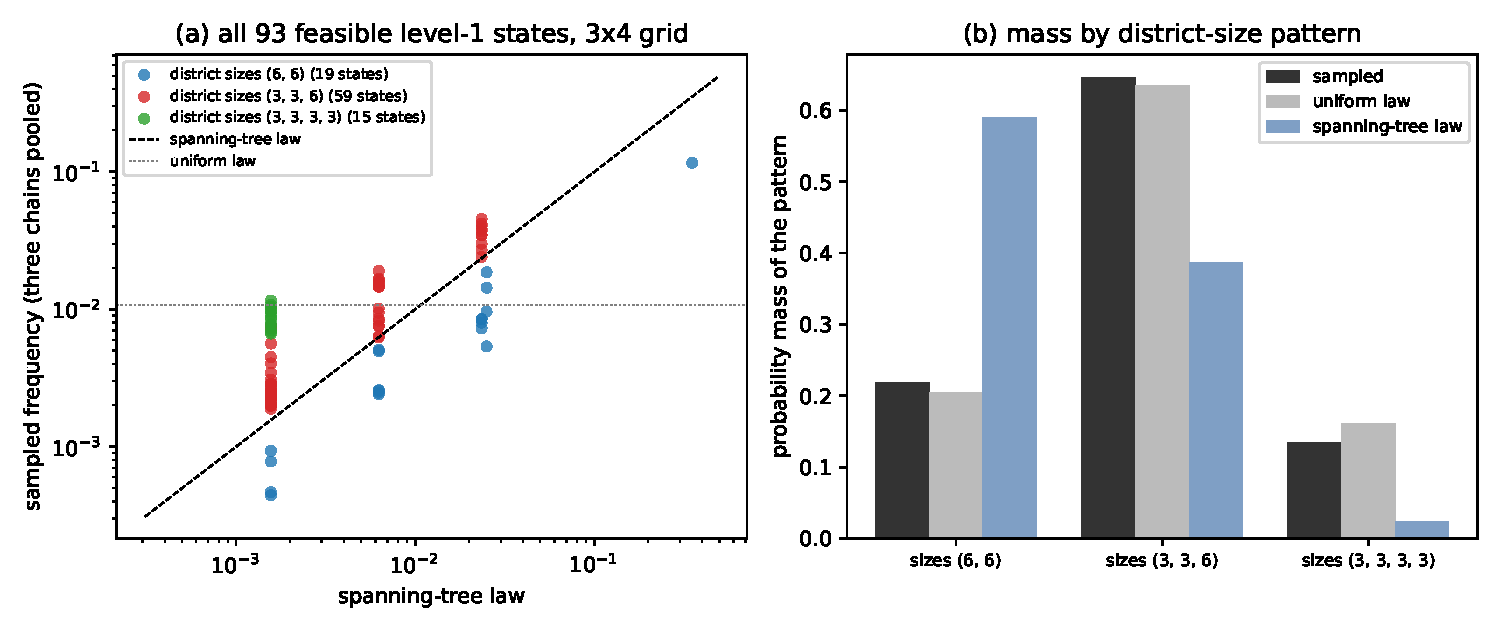
\includegraphics[width=\linewidth]{figures/validation/fig_enumeration_3x4.pdf}

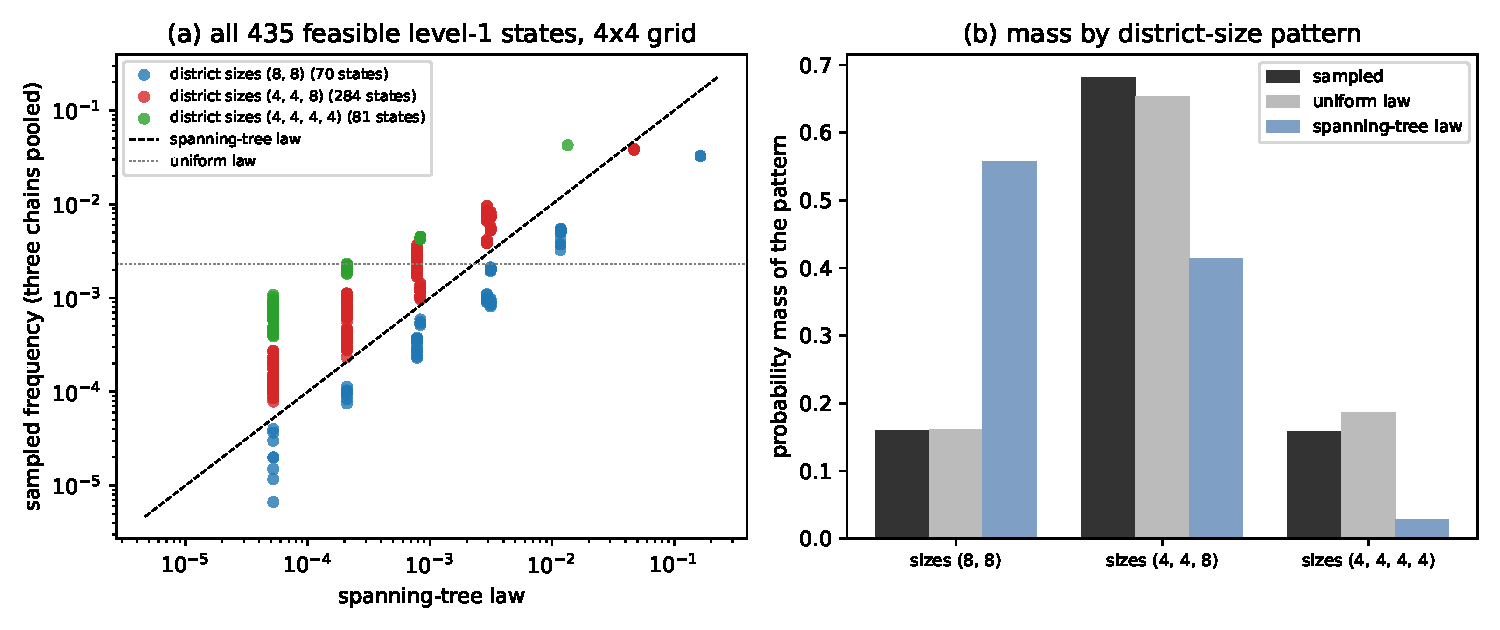
\includegraphics[width=\linewidth]{figures/validation/fig_enumeration_4x4.pdf}

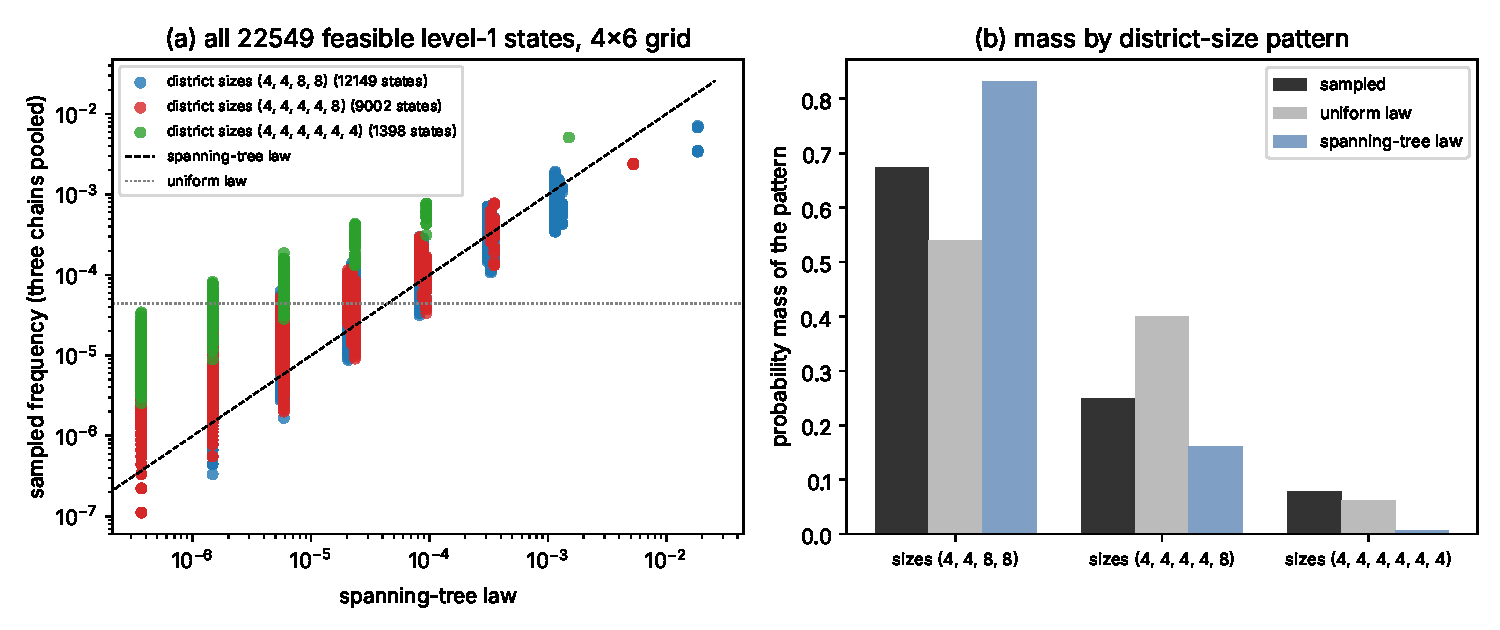
\includegraphics[width=\linewidth]{figures/validation/fig_enumeration_4x6.pdf}
\caption{Exact-enumeration validation. Top: the $3\times4$ grid; middle: the $4\times4$ grid; bottom: the $4\times6$ grid. (a)~Sampled frequency of each feasible level-1 state, three chains pooled, against the spanning-tree law, on logarithmic axes; the dotted line is the uniform law. (b)~Probability mass received by each district-size pattern under the sampled, uniform and spanning-tree laws.}
\label{fig:enumeration}
\end{figure}

Three facts follow from the counts. \emph{Soundness}: every visited state is feasible. Over $1.2$ million steps on the two small grids no chain produced a district without a candidate, a demand outside its window, a superdistrict with fewer than $\kappa^2_{\min}$ districts, or a disconnected part (the $3$--$4\%$ of proposals that would have left a superdistrict with a single district were rejected and counted). \emph{Support}: each chain visited all $93$ level-1 and all $119$ joint states of the $3\times4$ grid and all $435$ and $595$ of the $4\times4$ grid. \emph{Start-independence}: the total-variation distance between the empirical level-1 laws of any two chains is at most $0.012$ on the $3\times4$ grid and $0.024$ on the $4\times4$ grid, against noise floors of $0.011$ and $0.021$, and between the first and second halves of any one chain at most $0.016$ and $0.033$ against floors of $0.015$ and $0.029$. The empirical law is thus determined by the chain, not by its start, to within sampling noise.

The same holds for the joint (level-1, level-2) law. The total-variation distance between the joint laws of any two chains is at most $0.012$ and $0.026$ against floors of $0.011$ and $0.022$; the pooled joint law is at distance $0.46$ and $0.57$ from the uniform law on joint states; and the law of the level-2 partition given the level-1 partition, over the $15$ and $81$ level-1 states that admit more than one grouping, is at distance $0.45$ and $0.46$ from the uniform conditional law, averaged with the level-1 weights. On these instances $98\%$ and $97\%$ of the mass sits on states with a single superdistrict, hence the third instance. On the $4\times6$ grid, after $9$ million steps in all, the chains visited all but $14$ of the $22{,}549$ level-1 states, fewer than the $53$ that an independent sample of the same size from the pooled law would leave unvisited, and all but $45$ of the $43{,}689$ joint states, and every visited state was feasible. The level-1 laws of any two chains differ by at most $0.050$ against a floor of $0.035$, the joint laws by at most $0.062$ against $0.047$, and the two halves of one chain by at most $0.069$ against $0.049$. The pooled level-1 law is at distance $0.59$ from the uniform law and $0.32$ from the spanning-tree law, and the joint law at $0.62$ from the uniform law on joint states; $4\%$ of the mass has three superdistricts and the rest two. The law of level 2 given level 1, over the $12{,}344$ level-1 states with several groupings, is within $0.07$ of the uniform conditional law on average: $0.05$ on the $79\%$ of the mass where a level-1 plan admits exactly two groupings and $0.14$ where it admits three or more, against $0.45$ on the two small grids, where the few states with several groupings admit three each. Given the level-1 plan, the greedy supergraph recursion thus spreads its mass over the feasible groupings more evenly than the tree cut spreads it over level-1 plans, and the three chains agree on the joint law to within sampling noise.

The sampled law is neither uniform nor the spanning-tree law: its total-variation distance to the uniform law is $0.40$ on the $3\times4$ grid and $0.51$ on the $4\times4$ grid, and to the spanning-tree law $0.37$ and $0.43$ (Figure~\ref{fig:enumeration}). The figure shows what the law is instead. Across district-size patterns the chain distributes mass almost as the uniform law does: on the $3\times4$ grid the patterns $(3,3,6)$, $(3,3,3,3)$ and $(6,6)$ receive $0.65$, $0.14$ and $0.22$ against $0.63$, $0.16$ and $0.20$ under the uniform law, whereas the spanning-tree law puts $0.59$ of its mass on the two-district pattern. Within a pattern the sampled frequencies track the spanning-tree weights, the compactness preference that ReCom inherits from cutting random spanning trees, damped: the spanning-tree law conditioned on the pattern, with pattern masses taken from the chain, is within total-variation distance $0.11$ of the sampled law on the $3\times4$ grid and $0.24$ on the $4\times4$ grid, and the most and least frequent feasible states differ in sampled frequency by factors of $262$ and $6{,}381$, so the law is far from uniform within a pattern as well. On these two instances the recursion, which chooses the capacity of each extracted district uniformly among the admissible cuts of a random tree, sets a capacity mix close to the uniform one, and the spanning-tree geometry sets the law within a mix. On the $4\times6$ grid the picture changes: the patterns $(4,4,8,8)$, $(4,4,4,4,8)$ and $(4,4,4,4,4,4)$ receive $0.67, 0.25, 0.08$ against $0.54, 0.40, 0.06$ under the uniform law and $0.83, 0.16, 0.01$ under the spanning-tree law, so the mass across capacity mixes lies between the two reference laws (total-variation distance $0.15$ to the uniform and $0.16$ to the spanning-tree pattern masses, against $0.03$ to the uniform ones on the small grids), the spanning-tree law conditioned on the pattern is at distance $0.28$ from the sampled law, and the most and least frequent visited states differ by a factor of $63{,}724$. The characterization above is thus a property of the small instances, not of the chain; on larger instances the law is known through its support and the agreement of independently started chains only. On all three instances every unit has demand $100$, so every admissible district has demand exactly $c\,\bar d$, the running debt is identically zero and the debt-corrected windows coincide with the nominal ones; the enumeration therefore validates the tree-cut machinery and the support of the chain, not the debt mechanism, and the compounded windows of Proposition~\ref{prop:effective} cannot be exercised on it. The London readouts of Section~\ref{sec:exp-emergency} are readouts of the law of the same chain on a far larger instance, which these instances characterize only by analogy.

\FloatBarrier
\subsubsection{Multi-start agreement on large grids}
\label{sec:exp-multistart}

On grid\_10000 and grid\_50000, where enumeration is impossible, we run four chains from independently drawn zone-wise initial partitions, each carrying exactly $\lceil d/w \rceil$ units, and ask whether they forget their starts and agree with each other. The observables are the level-1 access cost $R^1 = \sum_{D \in \Pc^1} \sum_{v \in D} d_v\, \mathrm{d}(f^1(D), v)$, the base term of the median objective~\eqref{eq:milp-median} and the slow mode of the chain since one superdistrict is re-cut per step, the per-team demand spread $\max_D d(D)/c^1(D) - \min_D d(D)/c^1(D)$, the number of districts and, on the stored plans, the number of superdistricts, the cut-edge count and the share of unit-capacity districts. Agreement is the largest pairwise Kolmogorov--Smirnov distance between the post-burn-in distributions of an observable, compared with the same distance between the two halves of one chain; forgetting is the number of steps after which the share of the initial plan's boundary edges still in place reaches the share two independent plans have in common. Table~\ref{tab:multistart} reports the diagnostics.

\begin{table}[!htbp]
\centering
\footnotesize\setlength{\tabcolsep}{3pt}
\resizebox{\linewidth}{!}{\begin{tabular}{lrrrrrrrrrr}
\toprule
 & acceptance & $R^1$ & spread & $|\Pc^1|$ & $|\Pc^2|$ & cut edges & unit share & steps to forget & $\hat R(R^1)$ & ESS$(R^1)$ \\
\midrule
grid\_10000, between chains & $89.4$--$89.5\%$ & $0.042$ & $0.035$ & $0.044$ & $0.042$ & $0.077$ & $0.047$ & $180$--$360$ & $1.001$ & $1{,}740$ \\
\quad within one chain, halves & & $0.053$--$0.080$ & $0.040$--$0.077$ & $0.012$--$0.025$ & $0.029$--$0.069$ & $0.086$--$0.136$ & $0.071$--$0.097$ & & & \\
grid\_50000, between chains & $85.5$--$86.4\%$ & $0.090$ & $0.112$ & $0.052$ & $0.057$ & $0.095$ & $0.055$ & $540$--$780$ & $1.005$ & $647$ \\
\quad within one chain, halves & & $0.045$--$0.075$ & $0.043$--$0.115$ & $0.027$--$0.075$ & $0.048$--$0.096$ & $0.089$--$0.147$ & $0.049$--$0.108$ & & & \\
\bottomrule
\end{tabular}}
\caption{Multi-start diagnostics on the two large grids, four chains of $30{,}000$ steps each after a $20\%$ burn-in. The six middle columns are Kolmogorov--Smirnov distances: on the first row of each instance the largest pairwise distance among the four chains, on the second the range over chains of the distance between the two halves of one chain, for the level-1 access cost $R^1$, the per-team demand spread and the number of districts (every twentieth post-burn-in step), and for the number of superdistricts, the cut-edge count and the share of unit-capacity districts (stored plans, every $60$th step). ``Steps to forget'' is the range over chains of the number of steps after which the share of the initial boundary still in place is within $10\%$ of the share two independent plans have in common. $\hat R$ and ESS refer to $R^1$, the ESS pooled over the four chains.}
\label{tab:multistart}
\end{table}

On 10 of the twelve instance and observable pairs the chains differ from each other no more than one chain differs from itself; the exceptions are the number of districts on grid\_10000 ($0.044$ against a within-chain maximum of $0.025$) and $R^1$ on grid\_50000 ($0.090$ against a within-chain maximum of $0.075$). The series are autocorrelated, so the critical values of the two-sample test do not apply; at the effective sample size of $R^1$ per chain, $435$ and $162$, a difference in distribution below about $0.09$ and $0.15$ is not detectable, and the within-chain reference calibrates the noise of the statistic rather than proving convergence, since two halves of a chain confined to one region would agree as well; what the agreement of independently started chains adds is that the law reached does not depend on the start. Split-$\hat R$ is at most $1.005$. The chains forget their starts within $180$ to $360$ steps on grid\_10000 and $540$ to $780$ on grid\_50000, for plans of $38$ to $39$ and $85$ districts, after which the boundary share settles at the independent-plan value, $0.12$ and $0.09$. The rejections are supergraph trees without an admissible pendant subtree ($3$--$4\%$ and $7$--$7\%$ of proposals), demand failures of the supergraph recursion (at most $1.9\%$ and $2.5\%$), re-cuts that would leave a superdistrict with a single district (at most $5\%$ and $5\%$) and at most $19$ base-level failures per $30{,}000$ proposals, the price of a candidate set with $1.5$ sites per team, plus $14$ proposals in $120{,}000$ on grid\_50000 that failed the per-team safety check of Section~\ref{sec:recursive} after a cut; the larger grid has superdistricts of two to five units, so a re-cut of merged superdistricts more often draws a tree with no pendant subtree in the level-2 window. Every rejection is a repeated proposal, not an error; the four chains sample the same law, and the holding times of rejected proposals enter that law as quantified on the London instance (Section~\ref{sec:las-protocol}).

\FloatBarrier
\subsubsection{Scalability}\label{sec:exp-scalability}

Contribution~(iii) in Section~\ref{sec:intro} claims that FalCom handles graphs with up to $50{,}000$ basic units. A step re-cuts one superdistrict at level $1$ and re-partitions the supergraph of $k$ nodes at level $2$, so its cost has a local part, set by the merged subgraph $H$, and a global part, set by $k$. We run the sampler on all five grids for $T = 10{,}000$ steps and record, for every step, the wall-clock time, its split between the two parts, and the merged-subgraph size $|H| = \sum_{D \in D^2_j} |D|$ of the superdistrict $D^2_j$ that is re-partitioned. Travel times are Manhattan distances on grid coordinates evaluated lazily. Table~\ref{tab:scalability} reports the per-step cost.

\begin{table}[!htbp]
\centering
\small\setlength{\tabcolsep}{4pt}
\resizebox{\linewidth}{!}{\begin{tabular}{rrrrrrrrrr}
\toprule
$|V|$ & $|\mathcal{P}^1|$ & mean $|H|$ & $|H|/|V|$ & median $t_{\mathrm{step}}$ & mean, all proposals & $95$th pct & supergraph share & rejected & $10{,}000$ steps \\
\midrule
$100$ & $4$ & $89$ & $0.889$ & $3.6$\,ms & $4$\,ms & $8$\,ms & $5\%$ & $5\%$ & $0.7$\,min \\
$400$ & $7$ & $143$ & $0.356$ & $5.5$\,ms & $8$\,ms & $15$\,ms & $7\%$ & $8\%$ & $1.3$\,min \\
$1{,}000$ & $13$ & $212$ & $0.212$ & $9.3$\,ms & $16$\,ms & $24$\,ms & $9\%$ & $8\%$ & $2.6$\,min \\
$10{,}000$ & $38$ & $694$ & $0.069$ & $36.8$\,ms & $56$\,ms & $96$\,ms & $13\%$ & $10\%$ & $9.3$\,min \\
$50{,}000$ & $85$ & $1{,}566$ & $0.031$ & $106.5$\,ms & $167$\,ms & $248$\,ms & $19\%$ & $14\%$ & $27.9$\,min \\
\bottomrule
\end{tabular}}
\caption{Scalability sweep across the five synthetic grids, one chain of $10{,}000$ steps each. $|\mathcal{P}^1|$ is the median number of districts. The median and the $95$th percentile are over accepted steps; ``mean, all proposals'' is the wall-clock time per proposal including rejected ones. ``Supergraph share'' is the share of the step time spent re-partitioning the supergraph. Rejected steps are proposals whose recursion could not close within its retry budget or that would have violated $\kappa^2_{\min}$; they leave the state unchanged.}
\label{tab:scalability}
\end{table}

Across $|V| \in [100, 50{,}000]$, a $500$-fold range in which $k$ grows from $5$ to $112$, the median time of an accepted step rises from $3.6$ to $106$\,ms, a factor of $30$ or $|V|^{0.55}$, and the mean time per proposal including rejected ones by a factor of $41$, while $|H|/|V|$ falls from $0.89$ to $0.031$. The step time grows faster than the mean $|H|$, which rises by a factor of $18$; the difference is the supergraph re-partition, $5\%$ of a step on grid\_100 and $19\%$ on grid\_50000. A proposal that cannot close spends its whole retry budget of $M = 1{,}000$ trees, so on grid\_50000 the $10{,}000$ steps take $28$ minutes after $8$ seconds for the zone-wise initial partition; rejections rise from $5\%$ on grid\_100 to $14\%$ on grid\_50000, almost all of them supergraph tree failures ($8\%$) and re-cuts that would leave a superdistrict with one district ($4\%$), with at most $4$ base-level failures in $10{,}000$ proposals. Times are for the cloud container used for all runs in this section, roughly half the speed of the laptop of Section~\ref{sec:exp-milp}; the ratios, not the absolute times, are the claim.

With $w = 200\sqrt{|V|}$ the team count and the district size grow together, so the sweep cannot separate the two parts; holding the graph fixed and raising the team count does. On grid\_10000 rebuilt with $w = 10{,}000$, $5{,}000$ and $2{,}500$ at $1.5$ candidate sites per team, with $k = 101$ teams (152 candidates, $75$ districts) the zone-wise start closes in $4$ to $343$ seconds, the median accepted step takes $30$\,ms with $|H| \approx 351$, the supergraph recursion takes $40$ to $42$\% of a step and $12$ to $14$\% of proposals are rejected; with $k = 201$ teams (302 candidates, $148$ to $149$ districts) the zone-wise start closes in $49$ to $689$ seconds, the median accepted step takes $74$ to $78$\,ms with $|H| \approx 177$, the supergraph recursion takes $83$ to $86$\% of a step and $21$ to $24$\% of proposals are rejected; with $k = 401$ teams the zone-wise start, two zones of about $200$ teams each, did not close in twelve attempts (nineteen minutes), so the chain could not start. The local part is set by the merged region and the global part by $k$, and with many hundreds of teams the level-2 re-partition is the part that scales.

% =========================================================================
\FloatBarrier
\subsection{Comparison with Exact Optima}\label{sec:exp-milp}

The FalCom chain returns a distribution over feasible plans. To calibrate that distribution against an absolute reference, we solve the exact integer program of Section~\ref{sec:model} on the two smallest grids of Table~\ref{tab:grids}, grid\_100 and grid\_400, and compare the optimum with the best states FalCom visits when it is run as an optimizer. grid\_100 has $8$ candidate sites for $5$ teams and grid\_400 has $15$ sites for $10$ teams. Capacity bounds for the MILP runs are $c^1 \in [1, 2]$ and $c^2 \in [2, 5]$, and each open level-2 superdistrict must contain at least two open level-1 districts so that the hierarchy is non-trivial.

We equip FalCom with the \emph{disaggregated hierarchical median}, the sum of the demand-weighted distances of every unit to its level-1 and to its level-2 facility, in the spirit of the $p$--$q$ median of \citet{serra1993pq}:
    \begin{equation}\label{eq:milp-median}
      \min \quad
      \sum_{\ell \in L} \sum_{i \in V^1} \sum_{j \in F^\ell}
        d_i \, \mathrm{d}(i, j) \, x^\ell_{ij}
    \end{equation}
    where $\mathrm{d}(i,j)$ is the distance metric, Manhattan distance on grid coordinates for the synthetic instances. The level-1 term involves only $x^1$ and the level-2 term only $x^2$, so a level-1 facility is placed solely by the demand it serves within its own district and is never pulled toward its parent level-2 facility. Each level's facility therefore settles at the demand-weighted $1$-median of its (super)district. We deliberately avoid a coupled objective that penalizes level-1-to-level-2 facility proximity, since it would distort level-1 facilities away from the demand centers of their districts.

\paragraph{Protocol.}
The integer program is solved with Gurobi 13.0 on four threads of a laptop, once with the SHIR contiguity constraints of Appendix~\ref{app:shir} imposed at level~$1$ and once without any contiguity constraint. Every solve reached a proven optimum (MIP gap $10^{-6}$). The program uses the windows of constraint~\eqref{cons:balance} at $\varepsilon = 0.15$ around $w$, while FalCom's states satisfy the hierarchical rule of Proposition~\ref{prop:effective}, so the two feasible sets differ at level $1$: the optimum satisfies FalCom's rule, and the best FalCom states reported below have districts between $0.83$ and $1.23$ units of $w$, so not all of them are feasible for the program. The gap is a comparison of objective values, not of optima over one feasible set. In every solve with contiguity all superdistricts of the optimum are connected, so the optimum is also an optimum of the two-level model (Appendix~\ref{app:shir}). FalCom runs as an optimizer with the objective as its energy and a linear annealing schedule. At step $t$ of $T = 10{,}000$ an improving proposal is always accepted and a worsening one with probability $\exp(-\beta_t\,\Delta E/\sigma)$, where $\beta_t = t/T$ and $\sigma = E_{\mathrm{init}}/|V^1|$ is the initial energy per unit. With this scale about a thousand worsening moves are accepted per run on grid\_100, a tenth of them in the last third of the schedule, whereas on grid\_400 almost every accepted move falls in the first third. When the supergraph recursion fails, the optimizer re-cuts a superdistrict of the current level-2 partition instead of rejecting, in $7$ to $95$ of the $10{,}000$ steps of a run, so its proposal kernel differs slightly from the sampler's. Eight chains with different seeds run on each instance, and the best state seen by each, which is its final state on one grid\_100 seed and three grid\_400 seeds, is compared with the optimum. One run takes $15$ seconds on grid\_100 and $27$ seconds on grid\_400 on the laptop of the Gurobi runs, so the eight runs that reach the $7.5\%$ gap below take under four minutes against $830$ seconds for the proven optimum; the same run takes about a minute on the cloud container of Section~\ref{sec:exp-scalability}, which is therefore roughly twice as slow as the laptop.

\begin{table}[!htbp]
\centering
\footnotesize\setlength{\tabcolsep}{3pt}
\begin{tabular}{lrrrrrrr}
\toprule
instance & sites/teams & MILP (SHIR) & time & MILP, no SHIR & FalCom best & FalCom median & gap \\
\midrule
grid\_100 & $8$ / $5$ & $61{,}884$ & $1$\,s & $61{,}884$ & $62{,}427$ & $62{,}831$ & $0.9\%$ \\
grid\_400 & $15$ / $10$ & $352{,}810$ & $830$\,s & $352{,}785$ & $379{,}300$ & $397{,}836$ & $7.5\%$ \\
grid\_400, $T = 200{,}000$ & $15$ / $10$ & $352{,}810$ & $830$\,s & $352{,}785$ & $367{,}188$ & $380{,}101$ & $4.1\%$ \\
grid\_400\_dense & $23$ / $14$ & $316{,}234$ & $1{,}455$\,s & -- & -- & -- & -- \\
\bottomrule
\end{tabular}
\caption{Exact optima of objective~\eqref{eq:milp-median} with the SHIR contiguity constraints and without them, and the best and median best-seen states of FalCom run as an optimizer ($8$ seeds, $T = 10{,}000$ steps each unless stated; the median is the mean of the two middle seeds). ``Gap'' is the gap of the best FalCom state to the SHIR optimum. grid\_400\_dense is the capacity variant of the last paragraph.}
\label{tab:milp}
\end{table}

\begin{figure}[!htbp]
\centering
\begin{subfigure}[t]{0.495\linewidth}
  \centering
  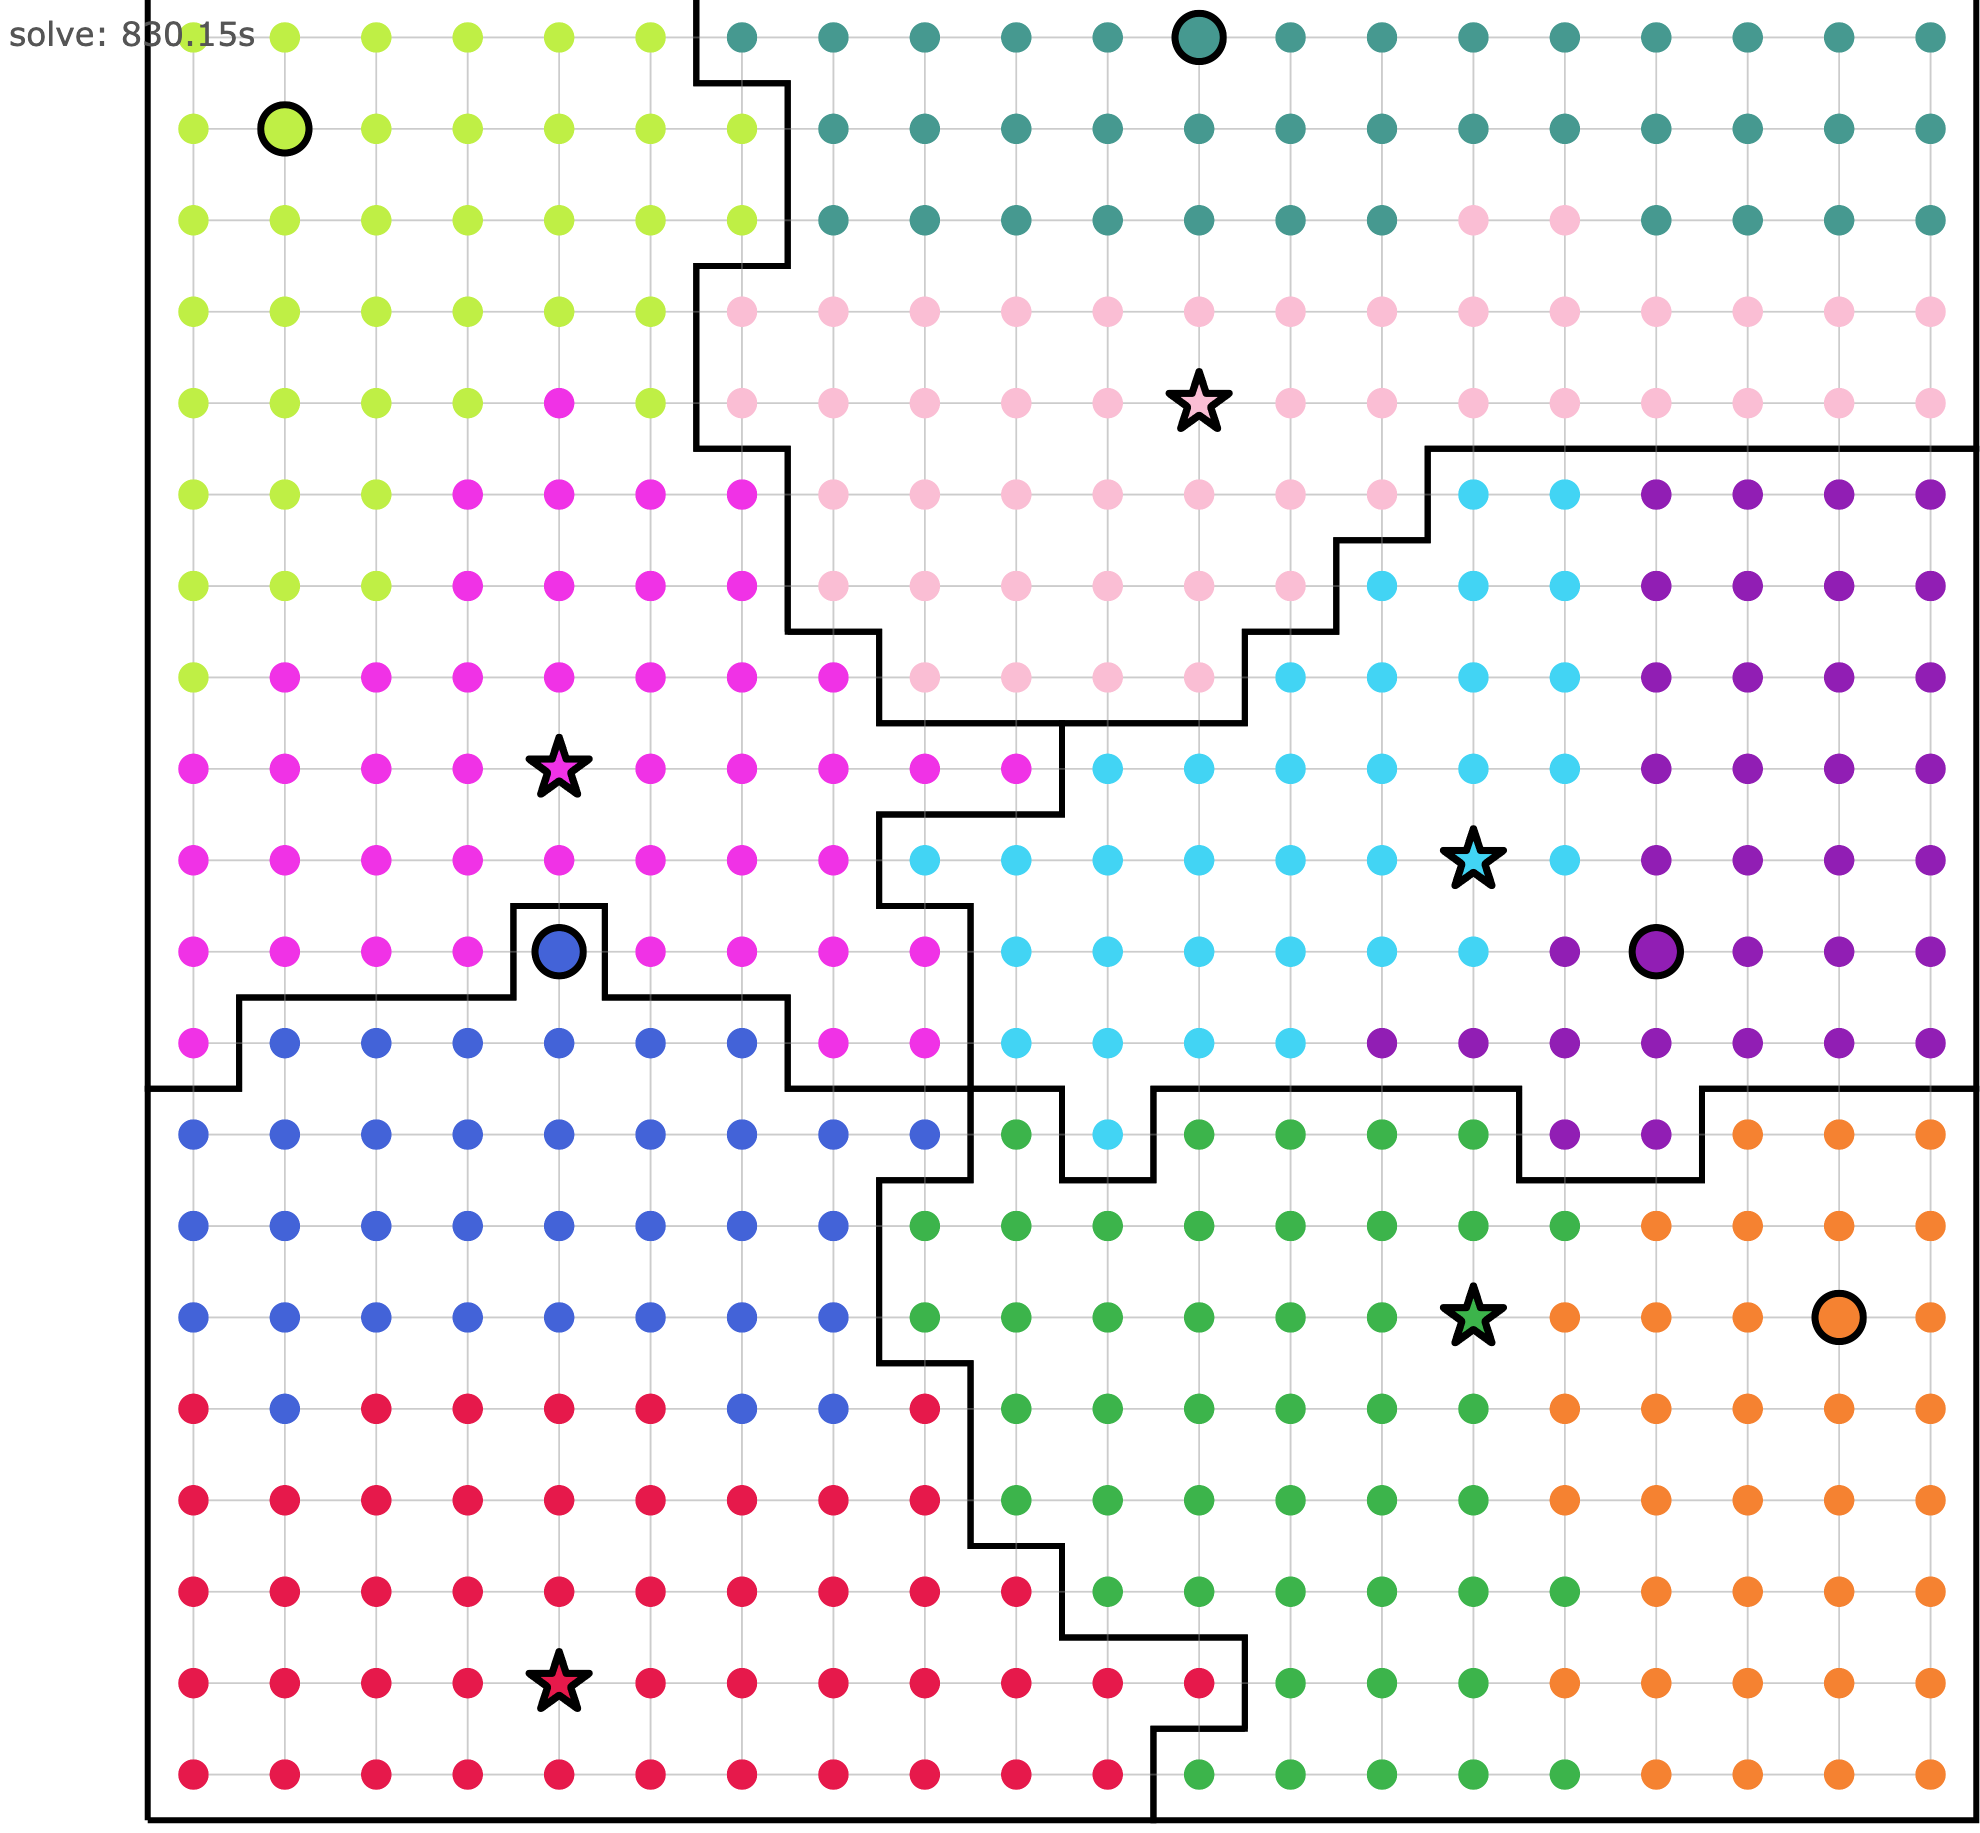
\includegraphics[width=\linewidth]{figures/milp/solution_400_median_shir_map.png}
  \caption{MILP optimum, $352{,}810$.}
  \label{fig:milp-400-a}
\end{subfigure}
\hfill
\begin{subfigure}[t]{0.495\linewidth}
  \centering
  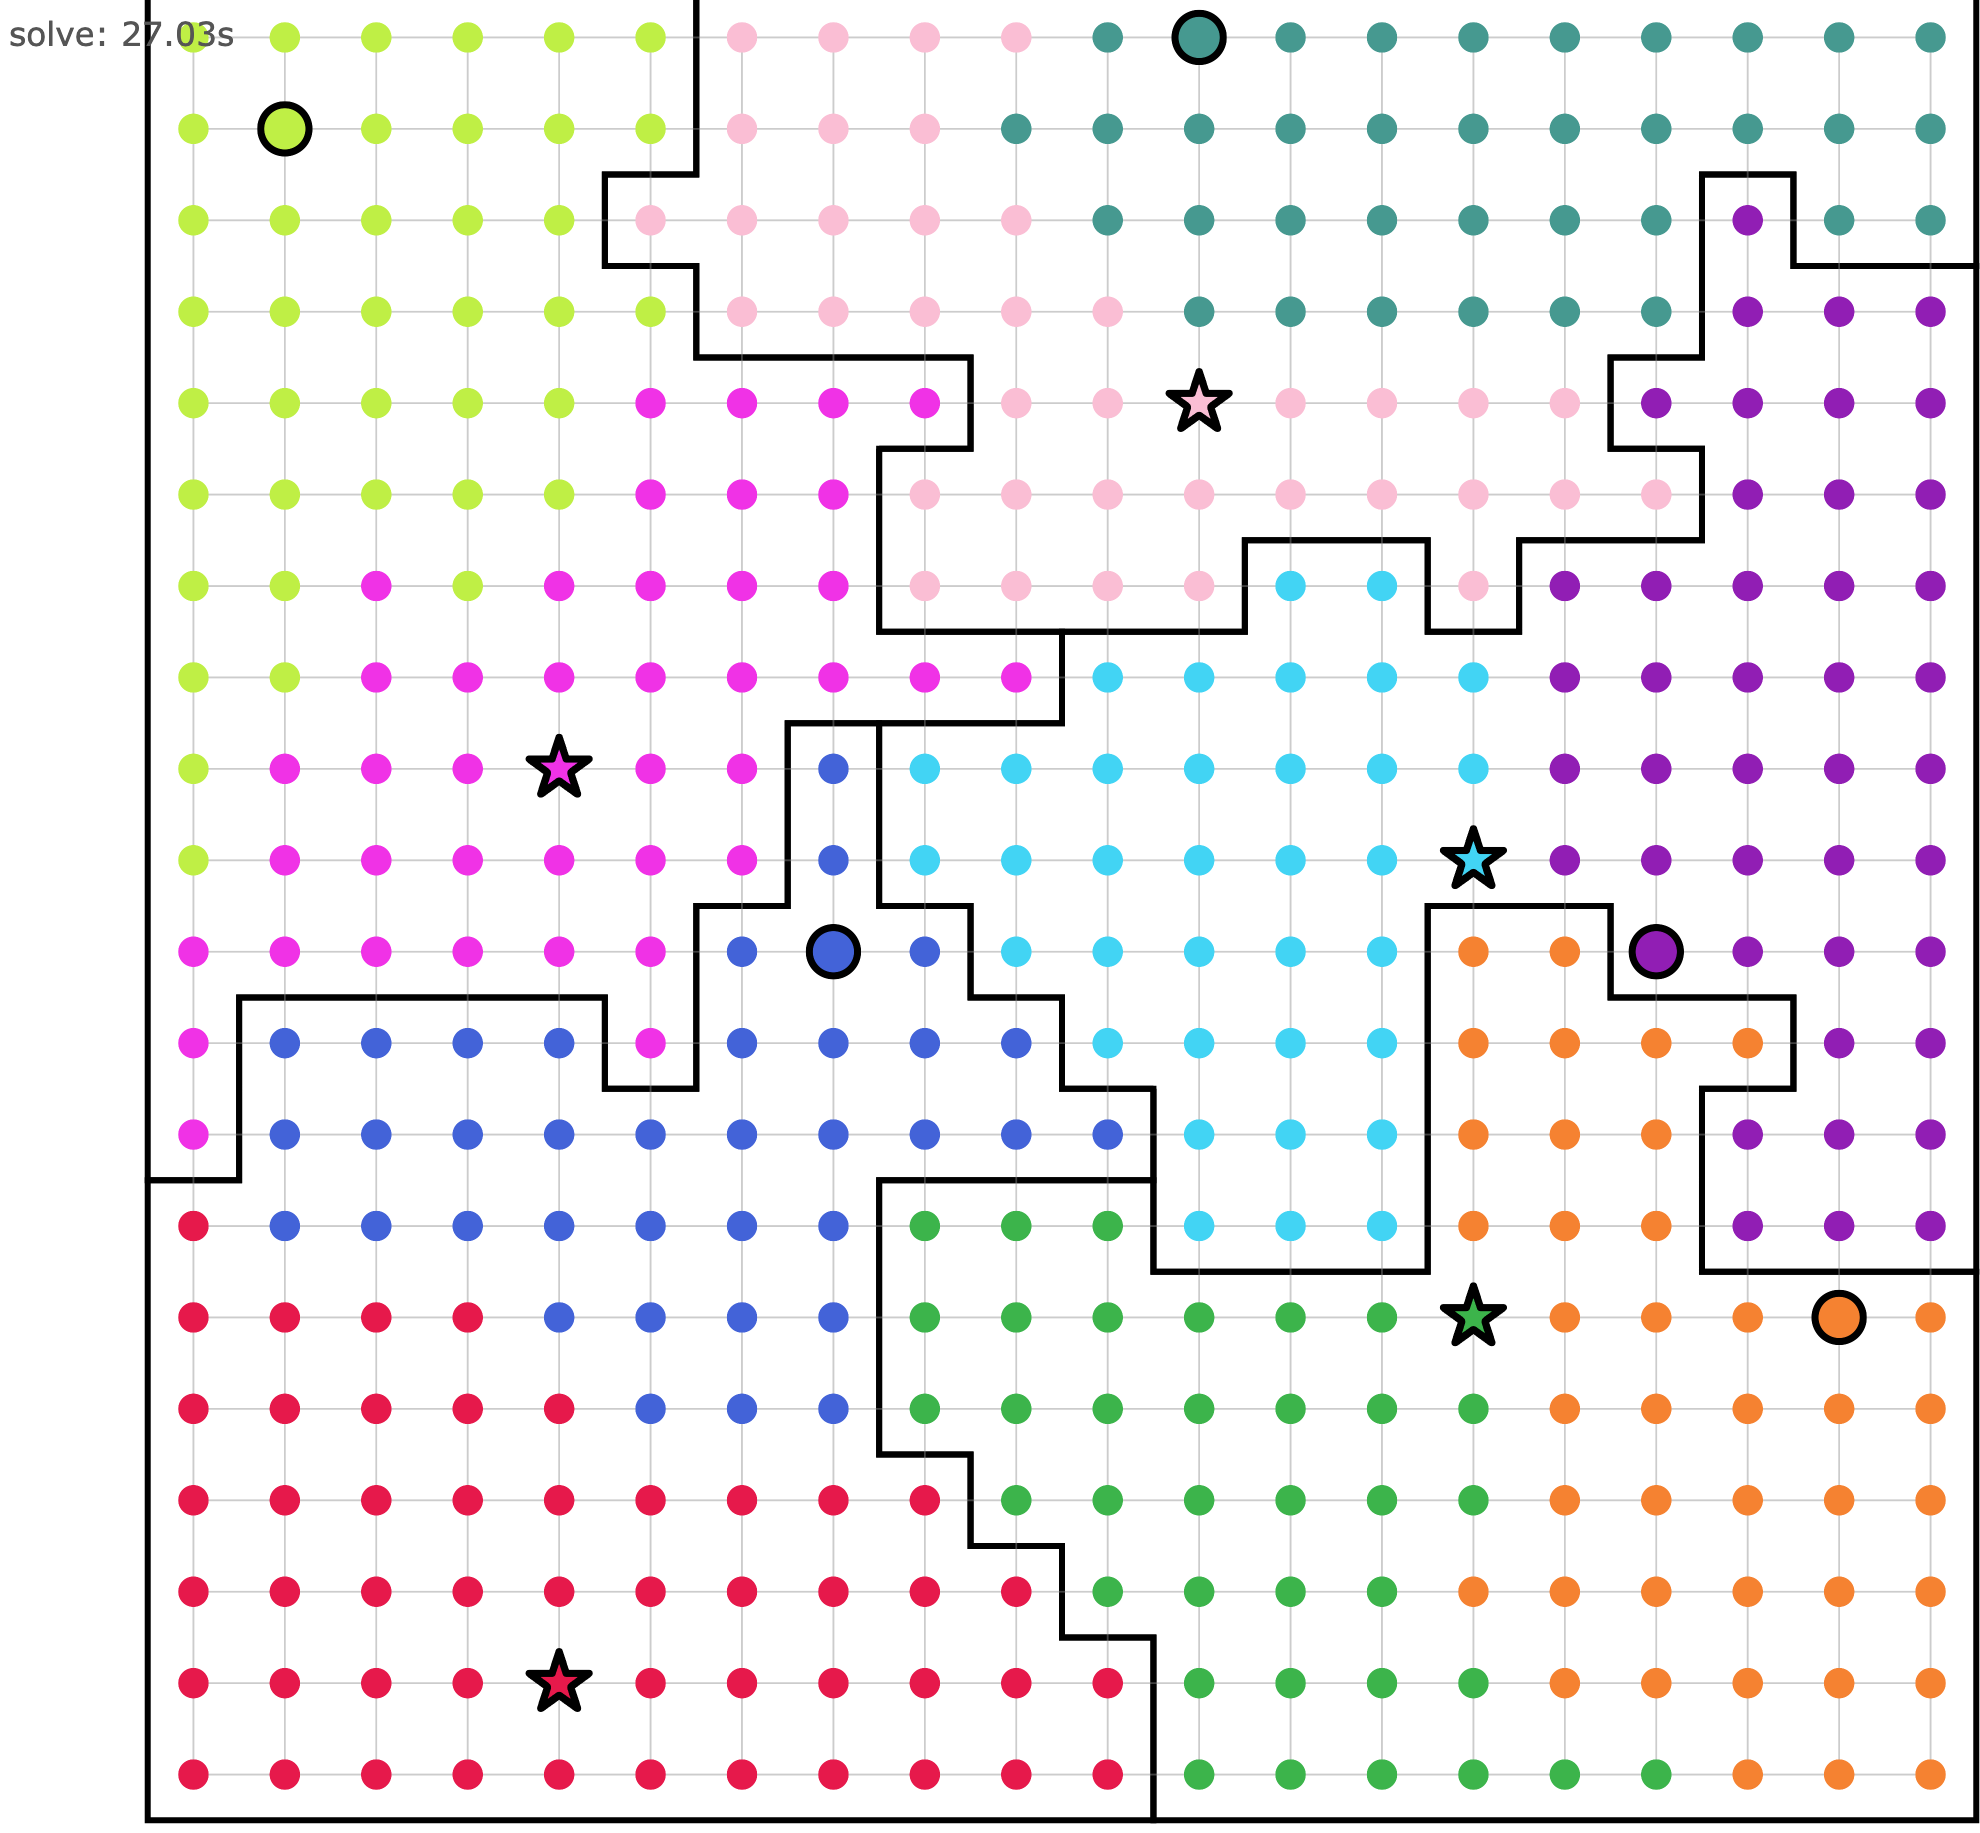
\includegraphics[width=\linewidth]{figures/milp/solution_400_falcom_multistart_best_final_map.png}
  \caption{Best FalCom state, $379{,}300$.}
  \label{fig:milp-400-b}
\end{subfigure}
\caption{grid\_400: the MILP optimum and the best FalCom state. Colours are level-1 districts, black lines superdistrict boundaries, circles open level-1 facilities and stars open level-2 facilities. Both plans open ten of the fifteen sites at one unit each in five superdistricts of two units.}
\label{fig:milp-400}
\end{figure}

\paragraph{Results.}
Table~\ref{tab:milp} and Figure~\ref{fig:milp-400} report the comparison. On grid\_100 the optimum opens five of the eight sites at one unit each in two superdistricts, with and without contiguity constraints, and the best FalCom state is $0.9\%$ above it, the worst of the eight seeds $2.6\%$. On grid\_400 the optimum opens ten of the fifteen sites as single-unit districts in five superdistricts. With ten of fifteen sites open, geometry nearly fixes which sites they are, and the best FalCom states share nine of them, so the comparison tests boundaries and grouping rather than site selection. The unconstrained optimum is $0.007\%$ cheaper and cuts one district in two, so contiguity is nearly free on this instance as well. The best FalCom state is $7.5\%$ above the optimum and the median seed $12.8\%$. Part of the gap is that the optimum uses the windows to their limits, with three districts at the upper edge $1.15\,w$ and one at the lower edge $0.85\,w$, where a sampled cut rarely lands. The rest is the optimizer mode, a crude annealer in which every proposal re-cuts a whole superdistrict, so that almost every accepted move falls in the first third of the schedule. A budget of $T = 200{,}000$, about an hour per seed, brings the best seed to $4.1\%$ and the median to $7.7\%$. The best FalCom state on each grid has the same capacity mix as the optimum, the same open level-2 facilities, and the same open level-1 facilities up to one site on grid\_400; across the eight seeds the open level-1 sites differ from the optimum's in at most three positions, and two of the eight grid\_400 seeds reproduce its level-2 facilities. The comparison establishes that the chain moves through the region of the optimum with the right structure, not that it is an optimizer, which the paper does not claim.

\paragraph{The role of capacity.}
With near-uniform demand the optimum uses single-unit districts only. A district of two units serves twice the demand from one site, which the median objective never prefers when a second site is available nearby. To exercise the capacity variable we build grid\_400\_dense from grid\_400 by raising two interior units to a demand of $1.4\,w = 5{,}600$, so that no single-unit district can hold either of them, and their eight neighbours to $300$, and by drawing $21$ sites at random and adding the two peak units as candidates, $23$ sites for its $14$ teams with the two peaks among them. The optimum with contiguity ($1{,}455$ seconds) opens twelve level-1 facilities, ten of one unit and two of two units around the peaks, grouped into six superdistricts of two or three units. Capacity is therefore chosen by demand concentration, as intended, and the sparse candidate set does not prevent it. FalCom itself cannot be run on this instance at the calibration of the sweep: the two peak units, of demand $1.4\,w$, exceed the granularity floor $\tau = \varepsilon w = 600$ of Section~\ref{sec:capacitated} by an order of magnitude, and the recursion did not build a feasible initial plan in eight seeds of fifty attempts each. A sampler calibration for such peaks needs a larger block or tolerance, which is how the London calibration of Section~\ref{sec:exp-emergency} places its heaviest unit ($1{,}526$) below the floor ($1{,}633$).


% =========================================================================
\FloatBarrier
\subsection{London Ambulance Service Case Study}
\label{sec:exp-emergency}
% =========================================================================
This case study evaluates \textsc{FalCom} on a large-scale hierarchical emergency medical service network based on the London Ambulance Service (LAS), the busiest urban ambulance service in the United Kingdom. LAS serves approximately $9$ million residents through $66$ ambulance stations organized into $21$ operational Groups within $5$ sectors. Unlike previous optimization studies on LAS~\citep{mccormack2015simulation}, which produce a single recommended plan, our goal is to characterize a reference distribution over feasible hierarchical configurations, the stationary law of the implemented chain, and to read the operational layout against it. We run FalCom on the real stations, with no artificial candidates, and use the ensemble in three ways: for the structure that most sampled plans share, for the role of each station, and as a reference against which the operational layout is measured. The last reading yields an upper bound, within a static assignment model and at this calibration, on what the current layout would give up by satisfying workload balance.

\subsubsection{Data}\label{sec:las-data}
The base graph $G^1$ has $|V^1| = 4{,}994$ nodes, the Lower layer Super Output Areas (LSOAs) of Greater London on 2021 boundaries, joined by $|E^1| = 14{,}550$ rook-adjacency edges (Figure~\ref{fig:las-instance}). LSOAs are the small-area unit of NHS planning and of the recent spatial-epidemiology work on LAS~\citep{murphy2024socio}. The level-1 candidate set $F^1$ is the set of $66$ LSOAs that contain an active LAS ambulance station, and nothing else. In the sampler any open station can serve as the level-2 facility of its superdistrict, by the rule given below; the $21$ documented Group headquarters~\citep{las_departments2025}, all of them active stations, enter only the benchmark state. Assumption~\ref{asm:facility-density} fails on this instance by a wide margin. The chain runs on the real stations because the counting predicate of Section~\ref{sec:capacitated} keeps the recursion closable, and the cost of the sparse candidate set is paid in rejections, which we report. Demand $d_v$ is the annual number of attended incidents in LSOA $v$: the 2010 to 2015 mean of the monthly borough totals that LAS publishes~\citep{las_incidents}, about $1.056$ million incidents a year across the $33$ boroughs, all of them in the catchment, apportioned to the LSOAs of each borough in proportion to the ONS mid-2024 population estimates~\citep{ons_sape2024}. The total is corroborated by the nearly $1.1$ million incidents attended in 2024/25~\citep{las_ar_2024_25}. Travel times are shortest-path driving times on the OpenStreetMap road network from every station to every LSOA centroid, with free-flow speeds scaled by $1.6$ for driving under lights and sirens; for the four LSOAs that the routing engine cannot reach from any station, one each in Hillingdon, Newham, Bromley and Camden, $0.1\%$ of demand and none hosting a station, straight-line distance at $25$ km/h is used. Variation within a borough is thus a proxy, daytime hot spots are smoothed into their residential surroundings, and the speed factor is an assumption. Appendix~\ref{app:slas} documents the assembly. Absolute energies and drive times inherit these approximations. A uniform speed factor rescales every road drive time, and hence every energy, by the same amount and leaves the ordering of plans by energy, the $1$-medians, the open frequencies and the ratio of the benchmark's energy to the ensemble's unchanged, up to the four fallback LSOAs, although not the eight-minute share; the demand proxy is tested directly in Section~\ref{sec:las-price} by repeating the study under a different within-borough apportionment.

\begin{figure}[!htbp]
\centering
\begin{subfigure}[t]{0.495\linewidth}
  \centering
  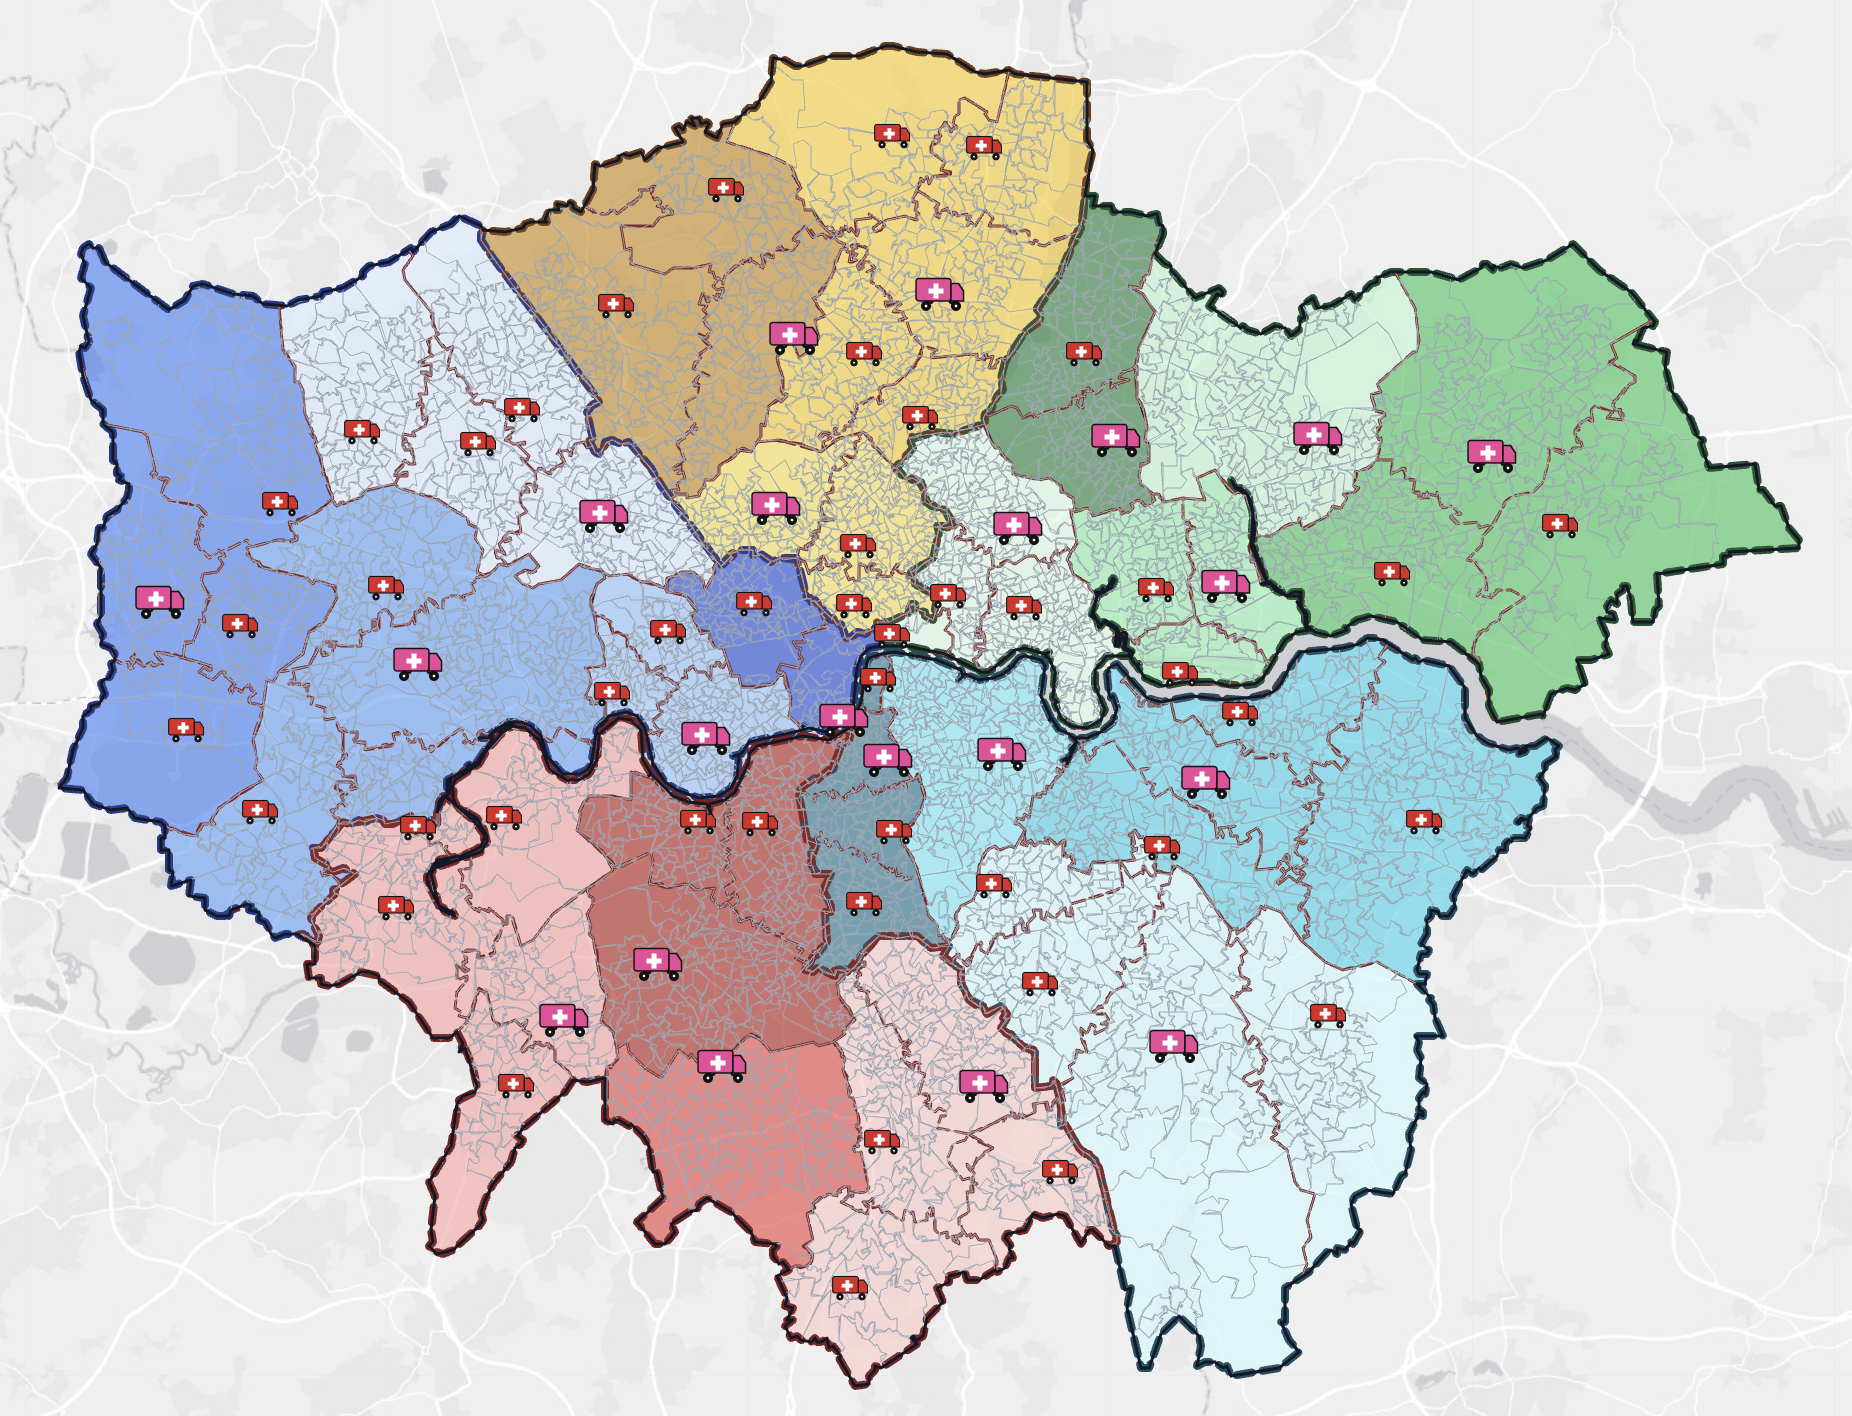
\includegraphics[width=\linewidth]{figures/las_map.png}
  \caption{LSOA polygons of the LAS catchment.}
  \label{fig:las-lsoas}
\end{subfigure}
\hfill
\begin{subfigure}[t]{0.495\linewidth}
  \centering
  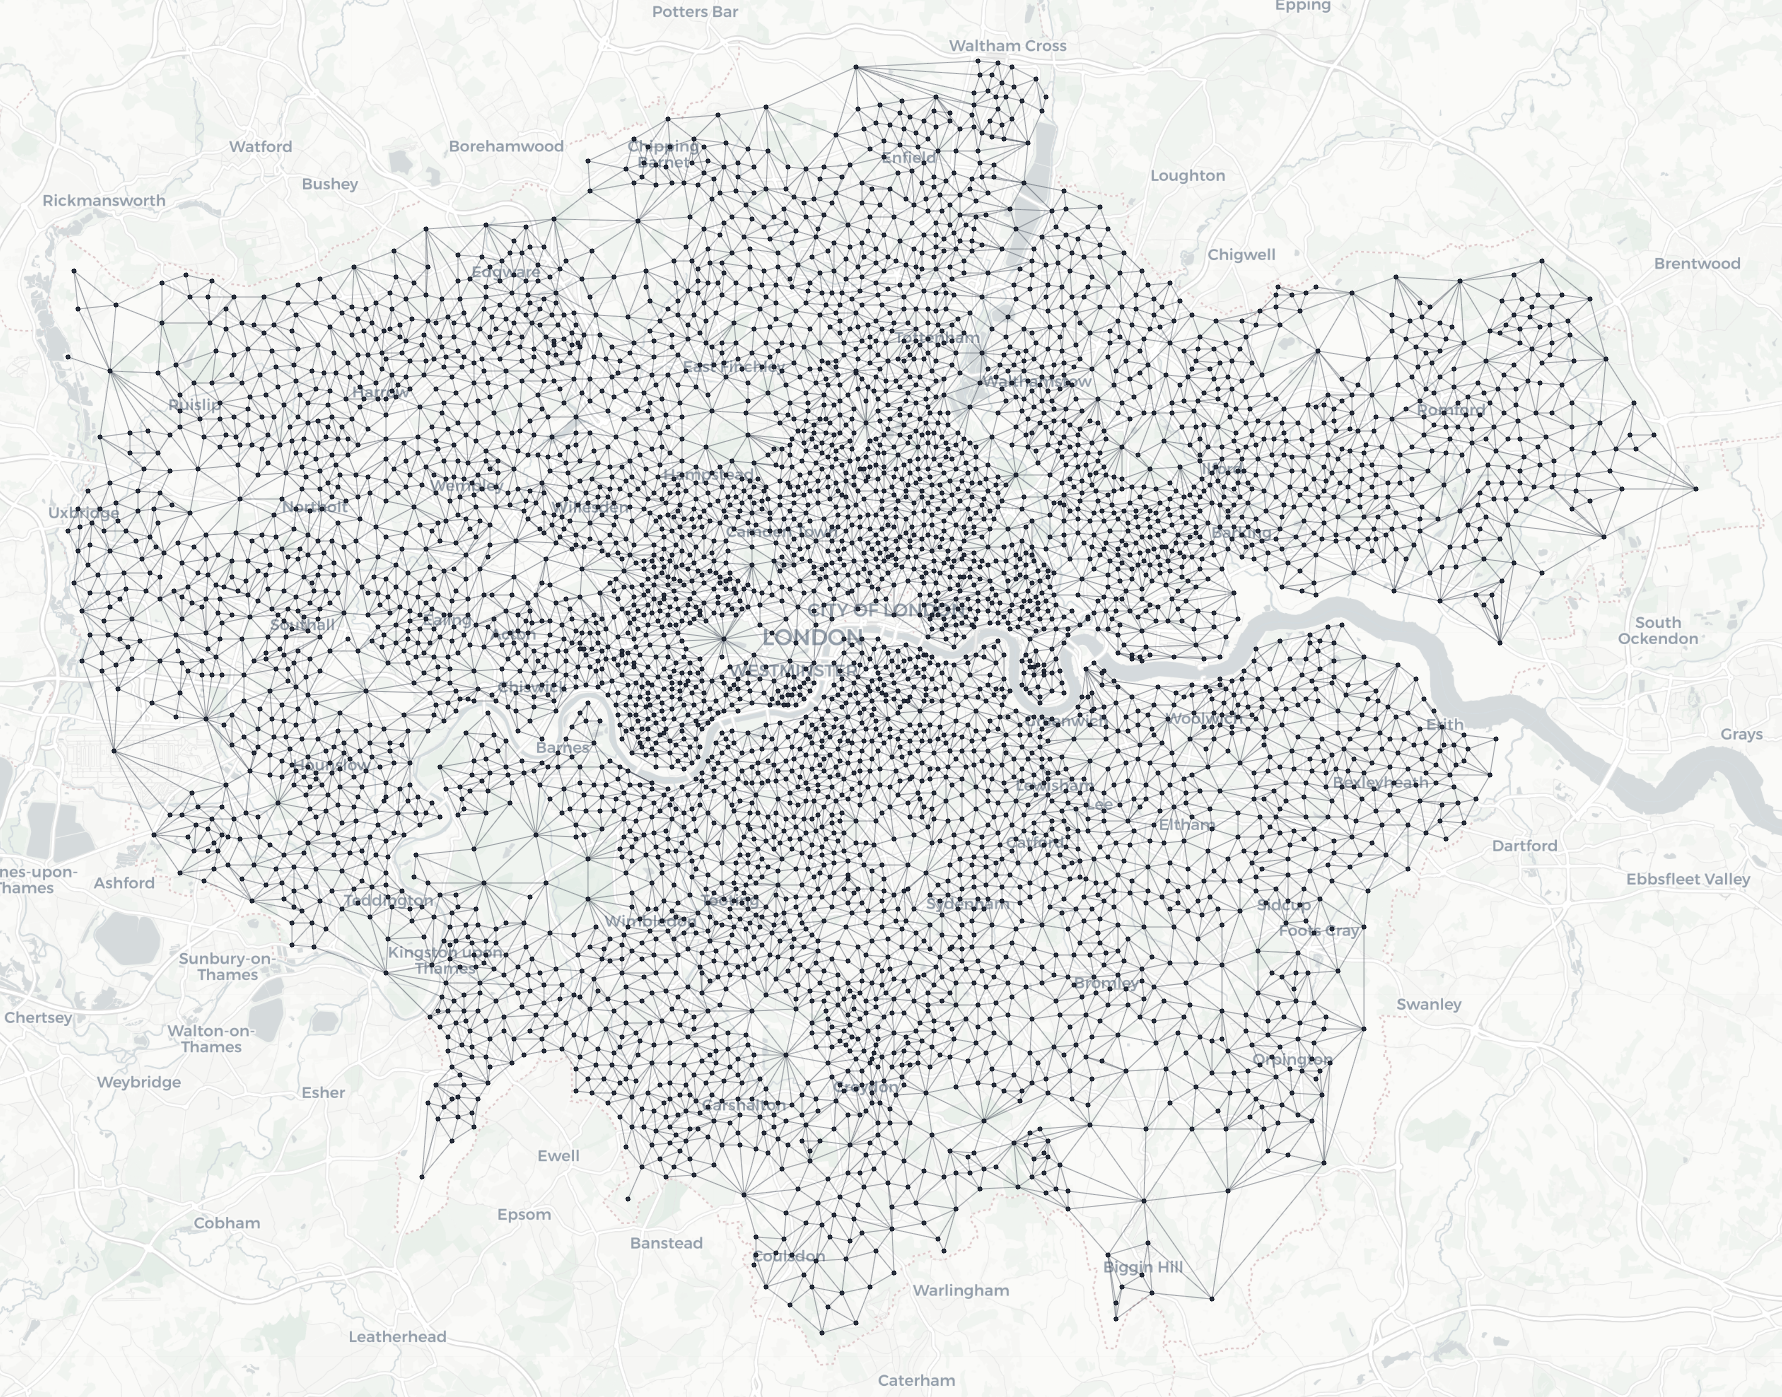
\includegraphics[width=\linewidth]{figures/las_dual_graph.png}
  \caption{Rook-adjacency dual graph $G^1$.}
  \label{fig:las-dual}
\end{subfigure}
\caption{The LAS instance. (\subref{fig:las-lsoas}) The $4{,}994$ LSOAs of the catchment; the $48$ Brentwood LSOAs are excluded. (\subref{fig:las-dual}) The dual graph $G^1$ on which the chain runs, with $14{,}550$ edges. Each node carries its integer annual demand.}
\label{fig:las-instance}
\end{figure}

\subsubsection{Calibration}\label{sec:las-calibration}
The capacity unit is a block of ambulances, and its size follows from the published productivity target and from the feasibility results of Appendix~\ref{app:debt}. The 2024/25 Annual Report~\citep{las_ar_2024_25} states a target of $5.2$ patients per crew per twelve-hour shift, rising to $5.4$. Five patients per shift, two shifts a day and $365$ days give $w_{\mathrm{amb}} = 3{,}650$ calls per ambulance per year. With $\varepsilon^1 = 0.15$, the granularity floor requires the per-team tolerance $\varepsilon^1 w_{\mathrm{unit}}$ to exceed the heaviest LSOA demand, $d_{\max} = 1{,}526$, so a unit must hold at least three ambulances. We take blocks of three and $w_{\mathrm{unit}} = 10{,}887$ calls per year, within $0.6\%$ of $3\,w_{\mathrm{amb}}$. The catchment's demand is $\lceil d / w_{\mathrm{unit}} \rceil = 97$ units, and every sampled state carries exactly $97$, as the coverage rule of Section~\ref{sec:rules} requires. Stations carry one to three units, the safe range of Corollary~\ref{cor:app-invariant}, and Groups carry two to six units with at least $\kappa^2_{\min} = 2$ stations each. Both tolerances are $0.15$. By Proposition~\ref{prop:effective}, a sampled one-unit station then serves between $0.72$ and $1.32$ units, a two-unit station between $1.51$ and $2.56$ and a three-unit station between $2.29$ and $3.79$, and every Group between $0.85$ and $1.15$ times its capacity; the loads realized over the stored plans range from $0.74$ to $1.32$ units per unit of capacity. The number of stations a plan opens is not an input. The calibration admits between $33$ and $66$ open stations, and the chain decides.

The unit is a demand quantum, not a vehicle count. The April 2025 fleet inventory lists $583$ double-crewed ambulances across the $21$ Groups, of which roughly seventy percent are on shift at any time, whereas $97$ blocks of three at the published target would be $291$ vehicles. The difference is the gap between the target and realized productivity, vehicles not crewed around the clock, and the 2010 to 2015 demand level. A calibration that bounds the capacity of each station by the fleet based there is a natural refinement that we leave to future work.

The level-2 facility of a superdistrict is the demand-weighted $1$-median among the stations open inside it, $F^2(s) = \{f^1(D) : D \in \Pc^1\}$, the dynamic rule of Section~\ref{sec:falcom}. The Group leg of the energy is therefore a measure of how compactly the stations of a superdistrict sit around their most central member. It is not a dispatch distance: LAS dispatches from its two Emergency Operations Centres rather than from the Group headquarters, so no vehicle travels from a headquarters to every incident of its Group. The operational comparison of Section~\ref{sec:las-price} rests on the station leg, and the Group leg is reported beside it as a descriptive statistic.

As a readout we use the disaggregated median energy
\[
  E(s) \;=\;
  \underbrace{\sum_{D \in \Pc^1} \sum_{v \in D} d_v \, t\bigl(v, f^1(D)\bigr)}_{E_1(s)}
  \;+\;
  \underbrace{\sum_{S \in \Pc^2} \sum_{v \in S} d_v \, t\bigl(v, f^2(S)\bigr)}_{E_2(s)},
\]
the drive-time form of objective~\eqref{eq:milp-median}, in demand-weighted minutes, with the station leg $E_1$ and the Group leg $E_2$ reported separately. Energy plays no part in the sampling, since every feasible proposal is accepted. It is evaluated on the samples, together with three metrics of the station leg, which describe catchment geometry under a static assignment of every LSOA to its catchment station: the demand-weighted mean drive time from the catchment station, its $90$th percentile, and the share of demand within eight minutes' drive of its catchment station.

\subsubsection{The operational layout as a benchmark}
We reconstruct the current operational layout as a state $s_{\mathrm{LAS}}$ in the same space. The five sectors are unions of boroughs, the five Integrated Care Systems of NHS England, and the 2025 list of departments~\citep{las_departments2025}, which lists the stations of each Group, together with the 2023 operational estate map~\citep{las_estate2023} assign each borough of a sector to one of its three to five Groups, so $89.8\%$ of LSOAs inherit their Group from a borough lookup. The remaining LSOAs lie in boroughs that the estate map splits between two Groups. We assign them by station Voronoi within the borough and correct $1.7\%$ by inspection of the map. Within a Group, every LSOA is served by its nearest station in straight-line distance. Seventeen LSOAs, $0.3\%$ of demand, are left detached from their station's catchment on $G^1$ by this rule, across bends of the Thames and railway land, and we move each to the neighbouring station of the same Group with which it shares the longest boundary. Appendix~\ref{app:slas} documents every step. All $66$ catchments and all $21$ Groups of $s_{\mathrm{LAS}}$ are connected on $G^1$.

The benchmark is not a member of the sampled space, for two reasons that are themselves findings. Three Groups (Deptford, Ilford and St Helier) contain a single station, which the rule $\kappa^2_{\min} = 2$ forbids, and the station loads of $s_{\mathrm{LAS}}$ range from $0.19$ to $4.68$ units, far outside the balance windows; its Group loads, $2.0$ to $6.7$ units, lie inside the level-2 windows, so at level $2$ the layout is load-feasible but not count-feasible. The comparison below is therefore between a contiguous hierarchical layout and a sample of plans that satisfy constraints the layout does not. It is also a comparison of static assignment models. Real dispatch sends the nearest available vehicle, not the home station of a fixed catchment, and LAS balances workload dynamically, so the drive-time figures describe catchment geometry rather than service performance, and the balance the windows impose is a static one.

\subsubsection{Protocol and convergence}\label{sec:las-protocol}
Four chains run for $T = 80{,}000$ steps each with uniform cut selection and unconditional acceptance. The initial plan of each chain is built sector by sector, each sector cut against its own per-unit target $d_Z / c_Z$ (Lemma~\ref{lem:app-telescoping}) with its share $c_Z$ of the $97$ units fixed by largest remainder, so that every initial state carries exactly $\lceil d/w \rceil$ units and the sector targets lie between $0.98$ and $1.03$ times $\bar d$, inside the level-2 window; it closes at the first or second attempt in under a second, where a global recursion on this instance rarely closes within its retry budget. The sector-wise start leaves the five sectors as the level-2 partition, far outside the level-2 windows; the first accepted step replaces it, and the initial state is excluded from every range reported below. Scalar traces are recorded at every step and the full plan, the station, superdistrict and capacity of every LSOA, every $40$ steps. The first $16{,}000$ steps are discarded as burn-in, so each chain contributes $1{,}600$ plans and the pooled ensemble holds $6{,}400$. A proposal whose recursion does not close, or that would leave a superdistrict with a single station, is rejected and the chain keeps its state. Each chain completes in $61$ to $62$ minutes on one core, $21.5$ to $22.0$ steps per second.

Acceptance is $67.7\%$ to $68.0\%$, and the rejections are a supergraph phenomenon. In $25.6\%$ to $26.1\%$ of proposals none of the $1{,}000$ spanning trees drawn for the supergraph has a pendant subtree inside its window, a tree failure; in $0.3\%$ to $0.4\%$ the supergraph recursion reaches a residual outside the window of its remaining capacity, a demand failure, about one supergraph failure in a hundred; and in $5.9\%$ to $6.3\%$ the re-cut would leave the selected superdistrict with one station. The base-level recursion fails $10$ to $22$ times per chain, fewer than once in $3{,}000$ proposals. The counting predicate thus removes the failure that the sparse candidate set would otherwise cause, and the residual predicate removes the strandings that capacities and counts can detect; without it the same chains accepted $38\%$ of their proposals. What remains is the tree-structural failure of a greedy extraction over $43$ to $61$ supernodes of capacity one to three (Appendix~\ref{app:supergraph-correctness}).

The four chains agree after burn-in. Chain means of the energy lie within $0.4\%$ of each other, $9.66$ to $9.70$ million demand-weighted minutes against a within-chain standard deviation of $0.28$ to $0.30$ million. The largest pairwise Kolmogorov--Smirnov distance between chains, on every twentieth step, is $0.066$ for the energy, $0.037$ for the number of stations, $0.020$ for the number of Groups and $0.070$ for the number of cut edges, and split-$\hat R$ on the per-step series is at most $1.003$. The series are autocorrelated, so the critical values of the two-sample test do not apply; as a reference we use the same statistic between the two halves of one chain, which is $0.028$ to $0.073$ for the energy, $0.021$ to $0.067$ for the number of stations, $0.011$ to $0.039$ for the number of Groups and $0.022$ to $0.083$ for the cut-edge count. On every observable the chains differ from each other no more than each differs from itself. The reference calibrates the noise of the statistic; it cannot detect a region of the state space that all chains miss, which is why a chain from a different construction is added below. Effective sample sizes per chain, on the per-step series, range from about $400$ for the cut-edge count and the station-leg energy, the two slowest observables, to $2{,}200$ to $3{,}400$ for the number of Groups, so the $6{,}400$ stored plans are worth about $2{,}970$ independent draws for the energy and $1{,}850$ for the cut-edge count, and the frequencies below are quoted to the precision this supports. The chains forget their starts quickly. The share of each initial plan's district boundary still in place falls to its plateau of $0.20$ within $320$ to $520$ steps, and the plateau equals the share of one chain's boundary that a plan from another chain cuts, $0.20$, so a burn-in of $16{,}000$ steps is conservative by more than an order of magnitude. The agreement extends to the readouts reported below, which are computed per chain before pooling: the share of plans in which a given station is open differs between two chains by at most $0.08$ (mean absolute difference $0.02$ over stations), the share in which two open stations share a Group by at most $0.11$ (mean $0.003$ over pairs), and the contestedness of the LSOAs correlates at $0.96$ or better between any two chains. The Monte Carlo standard error of a station's open frequency, estimated from the four chains, is at most $0.016$, and $0.007$ for the median station.

Holding the state on rejection reweights the sampled law by the expected holding time, $1/a(s)$ for a state $s$ from which a proposal closes with probability $a(s)$ (Section~\ref{sec:convergence-status}). On this instance $a(s)$ is not constant. Pooling the post-burn-in steps, acceptance rises from $0.61$ in states with $46$ open stations to $0.73$ in states with $58$, because a plan with fewer and larger supernodes is harder to re-partition, so the expected holding time falls from $1.64$ steps to $1.37$ and the time law tilts toward plans with fewer open stations; the rejection probability is $0.334$ after a rejected step against $0.315$ after an accepted one. The tilt is small in its effects. Weighting each stored plan by the inverse length of the visit it belongs to, which recovers the law of the jump chain, moves the mean number of open stations from $52.48$ to $52.54$, the capacity shares by at most $0.002$ and the open frequency of any station by at most $0.008$ (mean $0.002$); one station at the threshold, Chiswick, moves from $0.894$ to $0.900$ and joins the set open in more than $90\%$ of plans. We report the time law, which is what the chain samples, and note that the retry budget $M$ enters it through $a(s)$.

%% G7-START
The four chains share the sector-wise construction, so a fifth chain of $80{,}000$ steps was started from a structurally different state, an initial plan built inside the $21$ real Groups (the three single-station Groups merged into their neighbours, $18$ zones instead of five). It forgets its start within $480$ steps, to the same plateau of $0.20$, and after burn-in its largest Kolmogorov--Smirnov distance to any of the four sector-start chains is $0.044$ for the energy, $0.033$ for the number of stations, $0.018$ for the number of Groups and $0.081$ for the cut-edge count, against $0.066$, $0.037$, $0.020$ and $0.070$ among the four; split-$\hat R$ over the five chains is at most $1.005$. Its open frequencies differ from the pooled four by at most $0.05$ (mean $0.015$), against $0.045$ for any one of the four on its own; its set of stations open in more than $90\%$ of plans differs from theirs by five stations whose frequencies lie between $0.89$ and $0.92$ on one side or the other, as each of the four chains on its own differs from the pooled set by two to six such stations; and its mean energy, $9.69$ million, number of open stations, $52.4$, and adjusted Rand index against the real Groups, $0.28$, lie within the ranges of the four ($9.67$ to $9.69$ million, $52.4$ to $52.6$, $0.27$ to $0.28$). A start with a different level-2 structure thus reaches the same law.
%% G7-END

\subsubsection{What most sampled plans have in common}\label{sec:las-structure}
Every frequency in this section and the next is an estimate of a probability under $\pi_{\mathrm{FalCom}}$, the stationary law of the chain of Section~\ref{sec:falcom} as implemented, with its rejection rule and retry budget. That law is characterized only empirically (Section~\ref{sec:exp-enumeration}). It is supported on plans that satisfy the windows, it is not uniform over them, and on the enumerable instances it weights feasible plans by factors of up to $64{,}000$ on the largest enumerated instance, through spanning-tree counts, the recursion's capacity choices and the holding times just described. The readouts therefore come in three kinds. Statements about the benchmark, its infeasibility, its loads and its position relative to every sampled plan, do not depend on the law. Frequencies, how often an edge is cut, a station open or two stations grouped, do, and the replications of Section~\ref{sec:las-price} show which of them are stable under a change of tolerance and of demand proxy. Group readouts depend in addition on the level-2 construction, the greedy sequential recursion of Section~\ref{sec:recursive}, whose law is validated against enumeration only on small instances.

The ensemble separates the geography that most sampled plans reproduce from the choices that remain open. Over the $6{,}400$ plans, no edge of $G^1$ is cut by a station boundary in more than $44\%$ of them. $12.1\%$ of the $14{,}550$ edges are cut in fewer than $10\%$ of plans and lie inside catchments in nearly every plan; the other $87.9\%$ are contested. Group boundaries are more constrained. $30.8\%$ of edges are interior at level $2$, no edge is cut in more than $34\%$ of plans, and the level-2 boundary frequency concentrates on a few corridors in inner north London and along the river that separate clusters of stations (Figure~\ref{fig:las-boundary}). Seen from the units, an LSOA is served by its most frequent station in $48.3\%$ of plans on average ($48.5\%$ weighted by demand). Only $17$ LSOAs, $0.3\%$, keep one station in more than $90\%$ of plans, and these are the host LSOAs of the $17$ stations open in more than $90\%$ of plans, which constraint~\eqref{cons:anchor} ties to their station; $58.9\%$ of LSOAs have no station that serves them in even half of the plans. The map of contestedness shows the pattern: a settled core around each station, contested ground between stations, and settled fringes where stations are scarce (Heathrow, Havering, the southern edge), which are settled by scarcity rather than by geography.

\begin{figure}[!htbp]
\centering
\begin{subfigure}[t]{\linewidth}
  \centering
  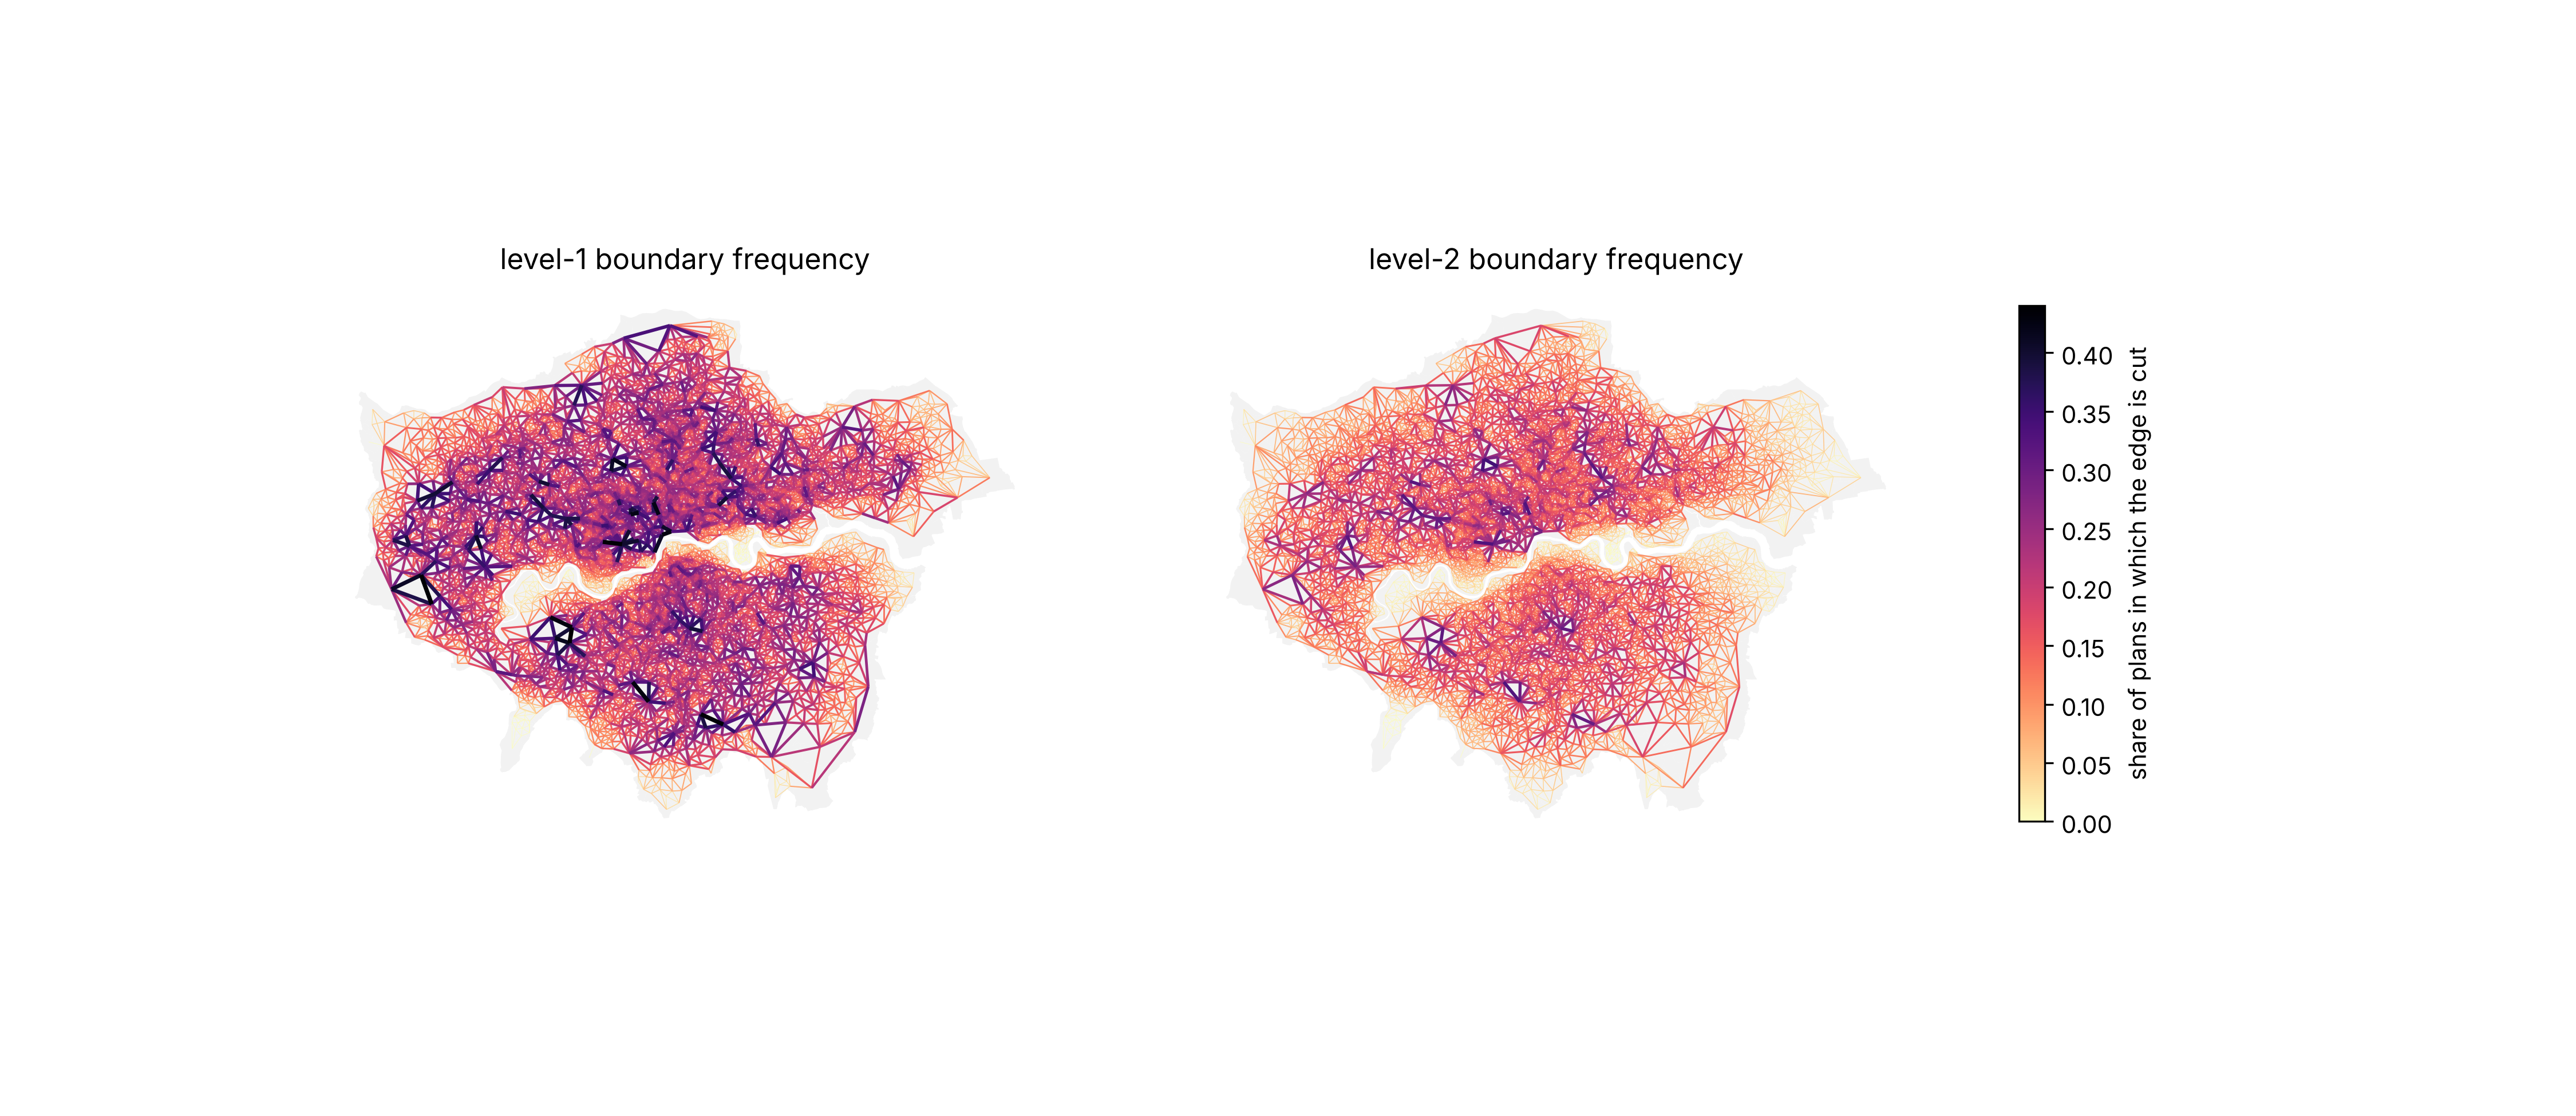
\includegraphics[width=\linewidth]{figures/las/fig_boundary_freq.png}
  \caption{Boundary-cut frequency at level 1 (left) and level 2 (right).}
  \label{fig:las-boundary-panels}
\end{subfigure}

\begin{subfigure}[t]{0.55\linewidth}
  \centering
  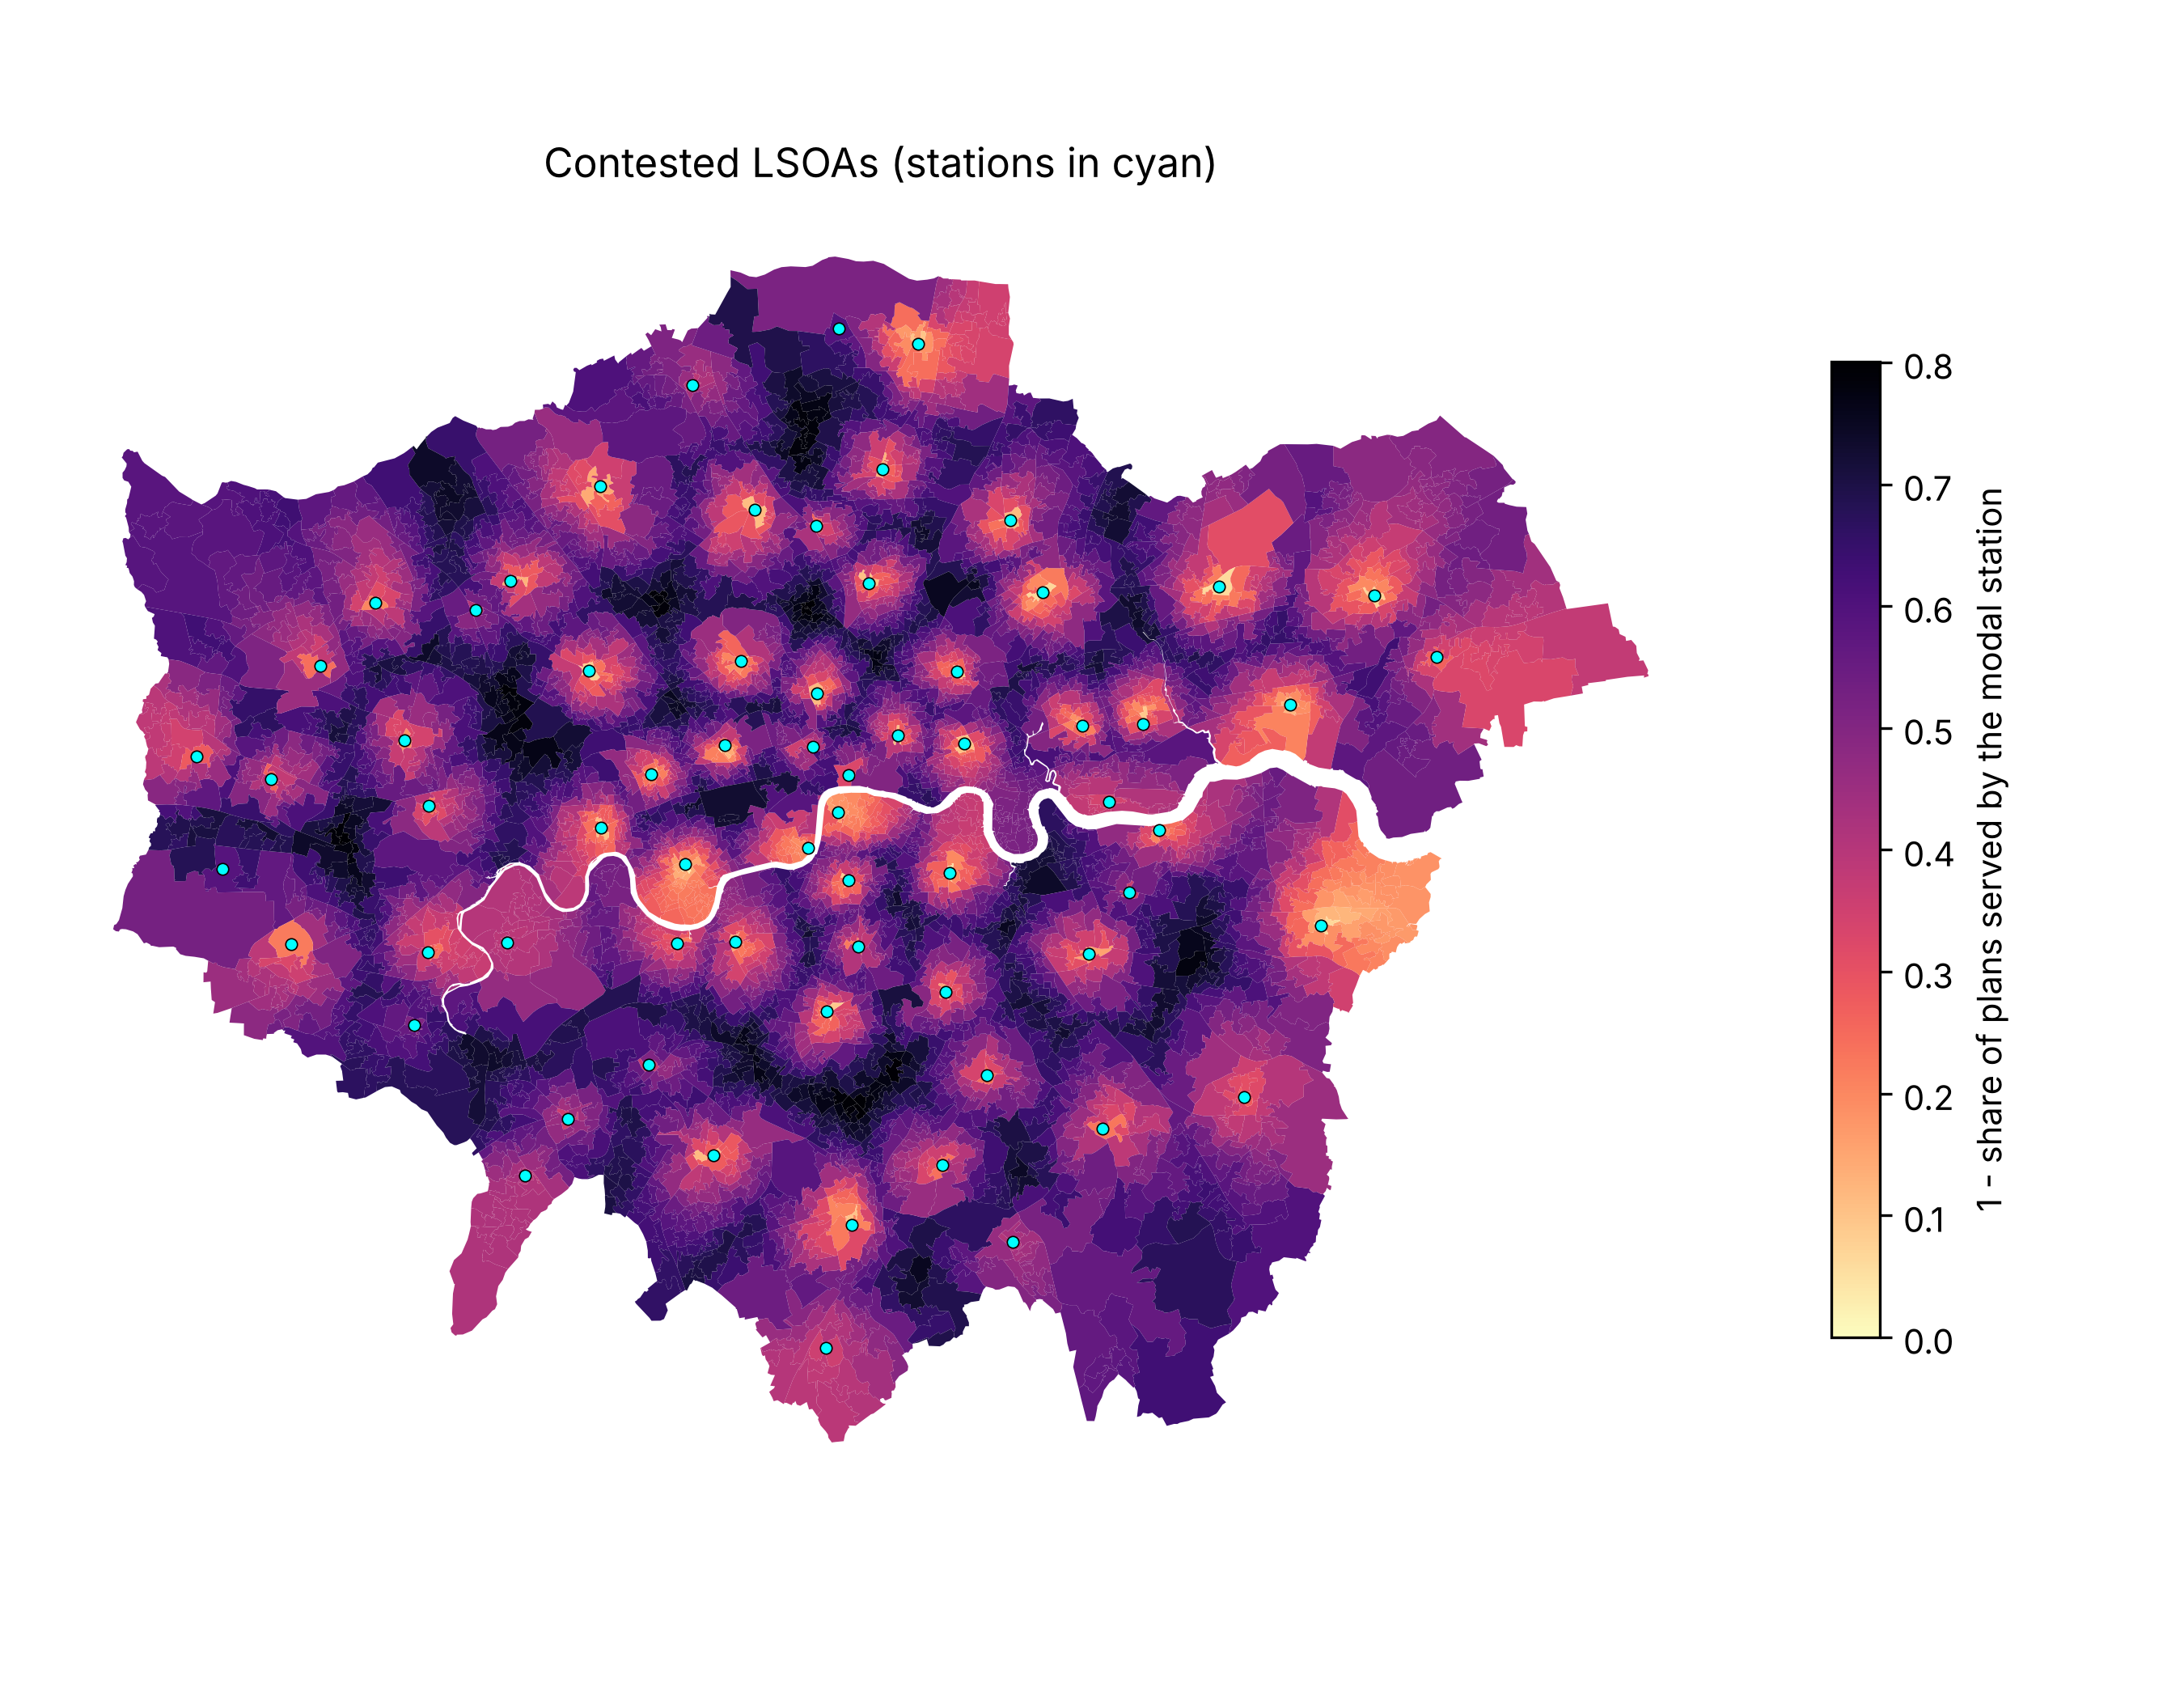
\includegraphics[width=\linewidth]{figures/las/fig_contested.png}
  \caption{Contested LSOAs.}
  \label{fig:las-contested}
\end{subfigure}
\caption{Boundaries and contested areas in the pooled ensemble. (\subref{fig:las-boundary-panels}) Share of plans in which each edge of $G^1$ is cut by a station boundary (left) or a Group boundary (right); darker and thicker is more often cut, and the colour scale runs to the largest observed frequency. (\subref{fig:las-contested}) One minus the share of plans in which an LSOA is served by its most frequent station. Stations in cyan.}
\label{fig:las-boundary}
\end{figure}

Because the candidates are the real stations, the ensemble also describes each station (Figure~\ref{fig:las-stations}). A plan opens $52.5$ stations on average, between $43$ and $61$, and between $49$ and $56$ in the central $90\%$ of plans. Seventeen stations are open in more than $90\%$ of plans, led by Fulham ($97\%$), St John's Wood ($96\%$), Ilford, Deptford and Barnehurst ($94\%$ each) and Whipps Cross ($93\%$). No station is open in fewer than $40\%$ of plans, and the median station is open in $83\%$. The least used sites are those whose surroundings cannot fill a unit, or that sit next to a stronger neighbour: Chase Farm ($40\%$), Heathrow Airport ($41\%$), Twickenham ($49\%$), New Addington and Wembley ($60\%$), and Tolworth, Barnet and Richmond ($61\%$). An open frequency counts how often the law opens a station. It says nothing about the cost of closing one, which the ensemble does not measure. Capacity follows density. Over all open stations, $42\%$ carry one unit, $31\%$ two and $27\%$ three. Inner stations such as St John's Wood, Ilford, Camden, Deptford and Brent carry three units in $37\%$ to $42\%$ of the plans in which they are open, and outer stations such as Tolworth, Richmond, Chase Farm, Heathrow Airport and New Addington carry one unit in $67\%$ to $77\%$ of theirs.

The sampled Groups recover part of the operational structure (Figure~\ref{fig:las-groups}). A plan has $22.3$ Groups on average, between $20$ and $24$ in the central $90\%$ of plans, against the $21$ real Groups. We measure co-membership as the share of plans in which two stations lie in the same superdistrict, among the plans in which both are open. Two stations of the same real Group share a superdistrict in $27\%$ of such plans, two stations of different Groups in $2\%$. Part of this contrast is distance, since stations far apart never share a superdistrict. The adjusted Rand index between a sampled grouping of the open stations and the real Groups is $0.28$ on average, between $0.17$ and $0.39$ in the central $90\%$ of plans and $0.28$ among the $1{,}255$ plans with exactly $21$ Groups; between two sampled plans from different chains it is $0.19$. The real Groups are thus recovered somewhat better than one sampled plan recovers another. They are one contiguous, capacity-feasible grouping among many that the geography admits, a typical member of the family rather than its mode. The pairs the ensemble keeps together most often inside a real Group are Hornchurch and Romford ($67\%$), Barnehurst and Woolwich ($55\%$), Becontree and Hornchurch ($52\%$), and Oval and Waterloo and Ponders End and Chase Farm ($49\%$ each). Equally strong are pairs that the real Groups separate: Barnehurst and St Pauls Cray ($49\%$, Greenwich and Bromley Groups), Richmond and Putney ($48\%$), Fulham and Westminster ($47\%$), Waterloo and Deptford ($42\%$) and Heathrow Airport and Feltham ($41\%$). Fourteen cross-Group pairs exceed $30\%$ against $29$ within-Group pairs. The cross-Group pairs are the associations a planner would examine first, since they mark Group boundaries that balanced plans tend not to draw.

\begin{figure}[!htbp]
\centering
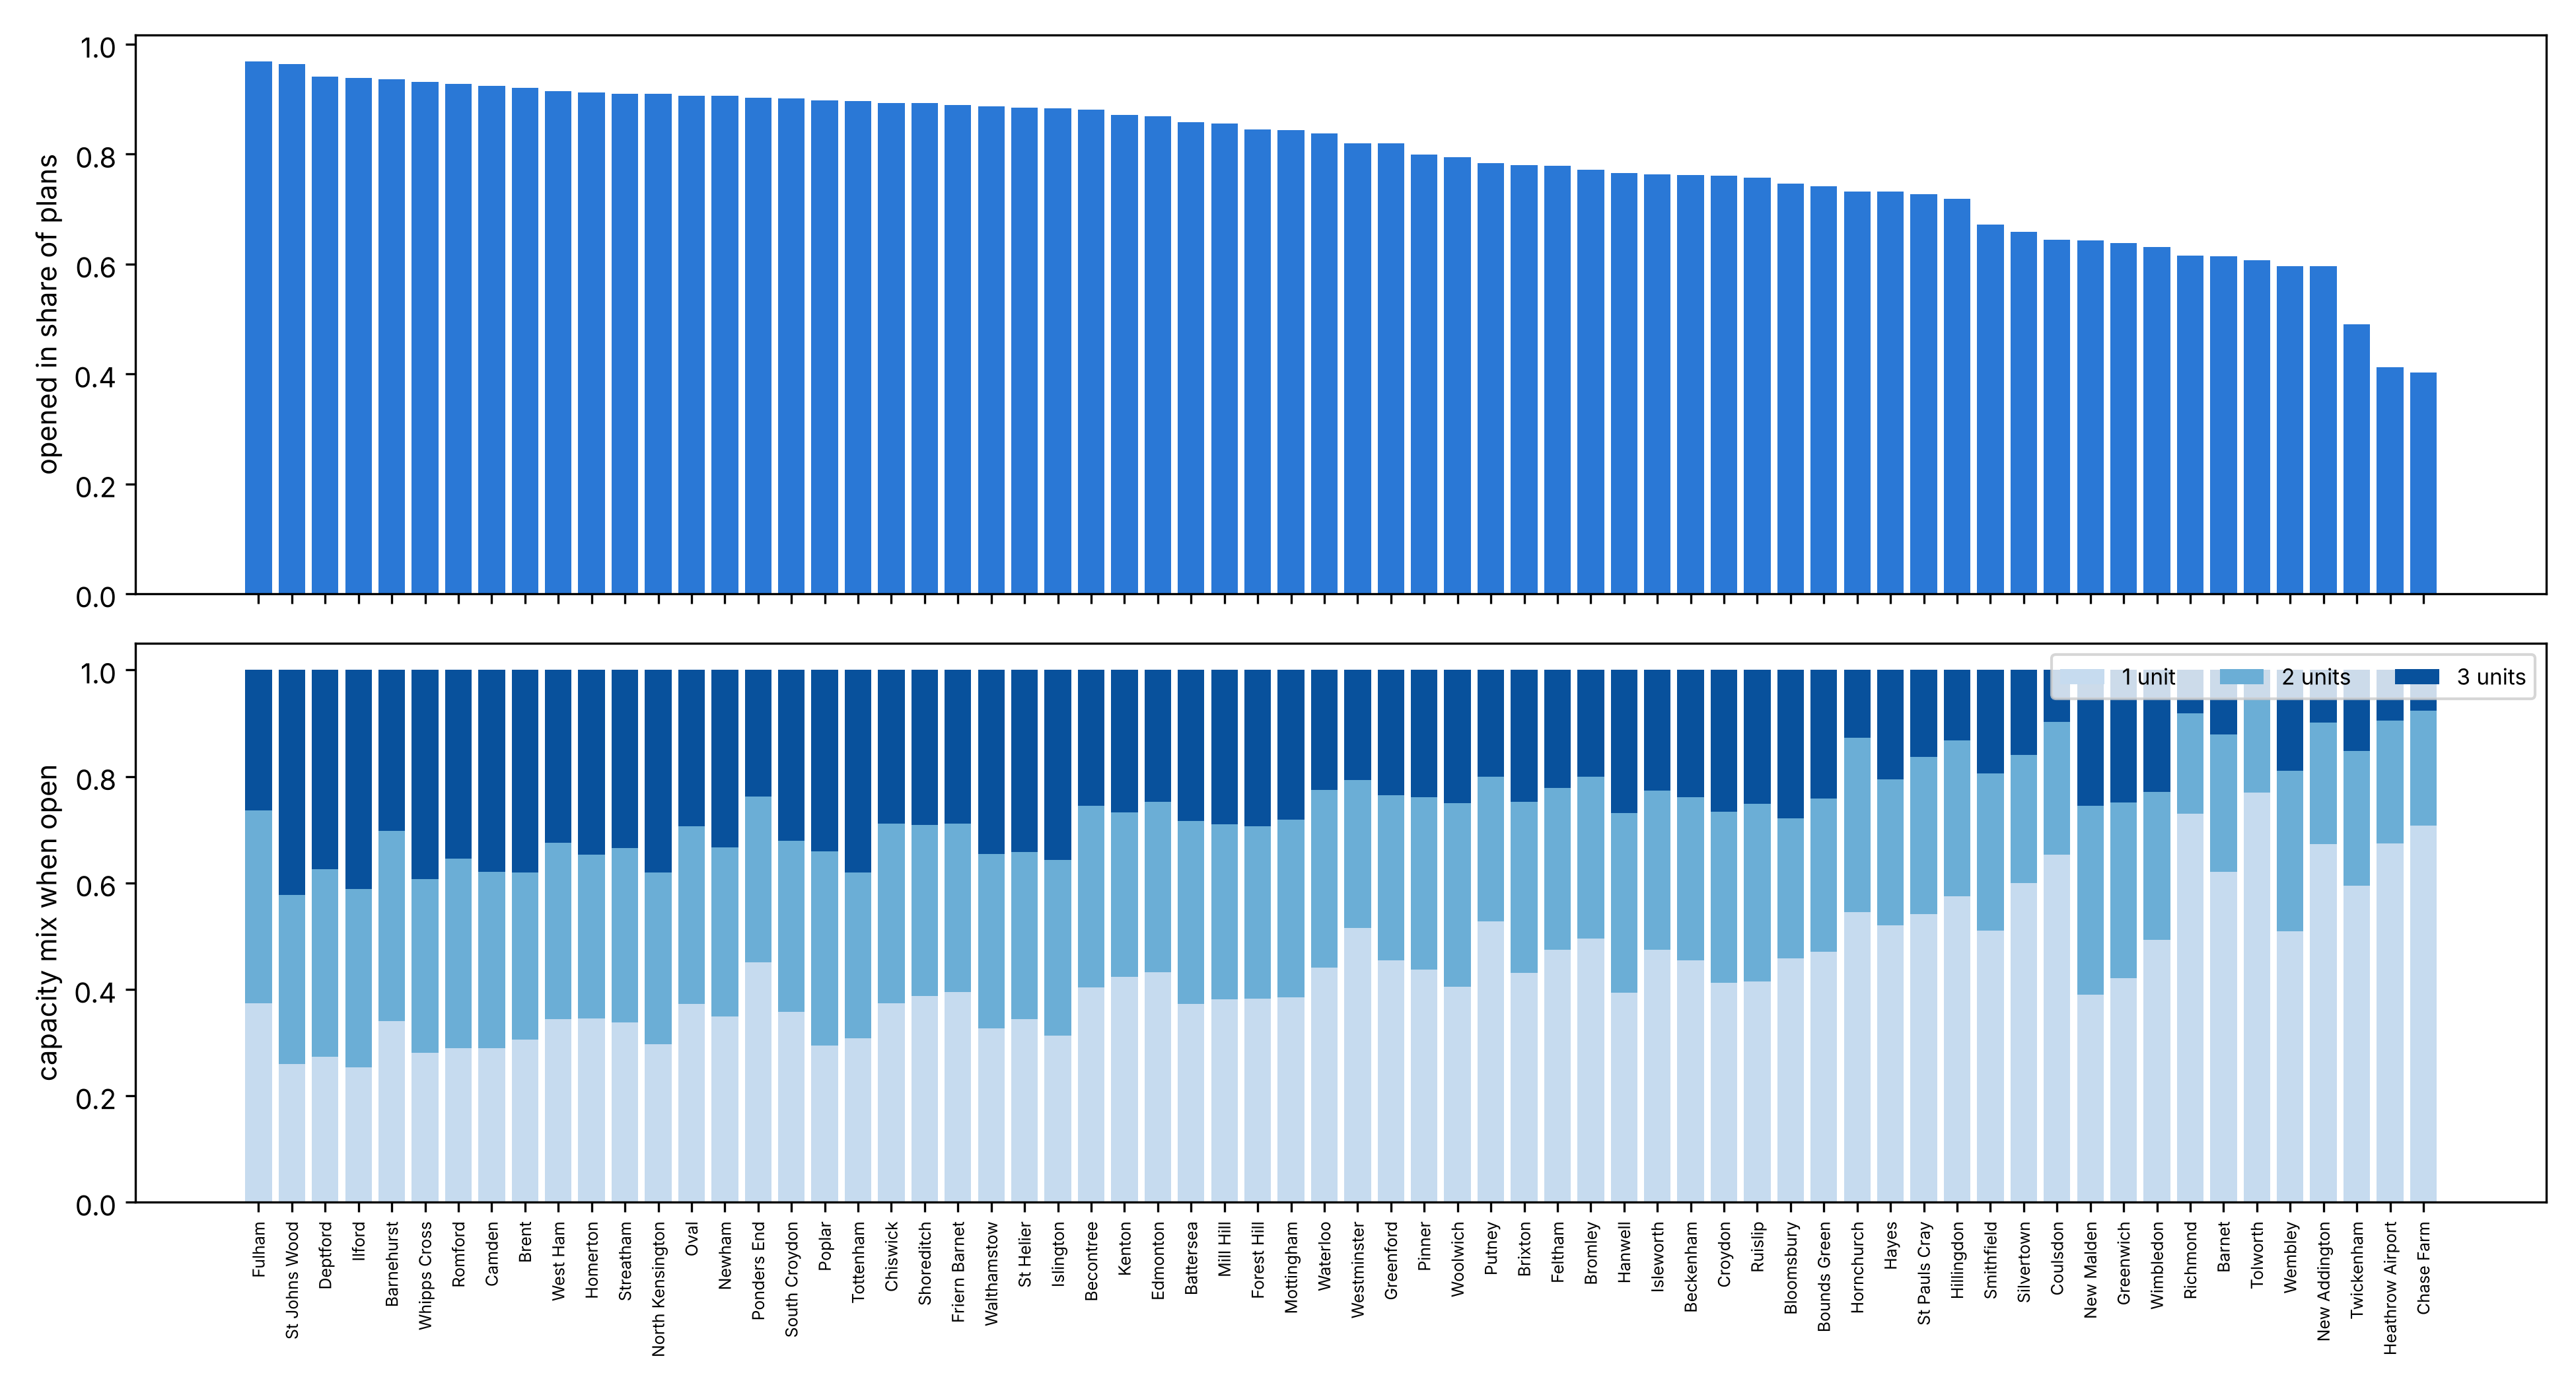
\includegraphics[width=\linewidth]{figures/las/fig_stations.png}
\caption{Top: share of plans in which each station is open, sorted. Bottom: capacity mix of each station in the plans in which it is open.}
\label{fig:las-stations}
\end{figure}

\begin{figure}[!htbp]
\centering
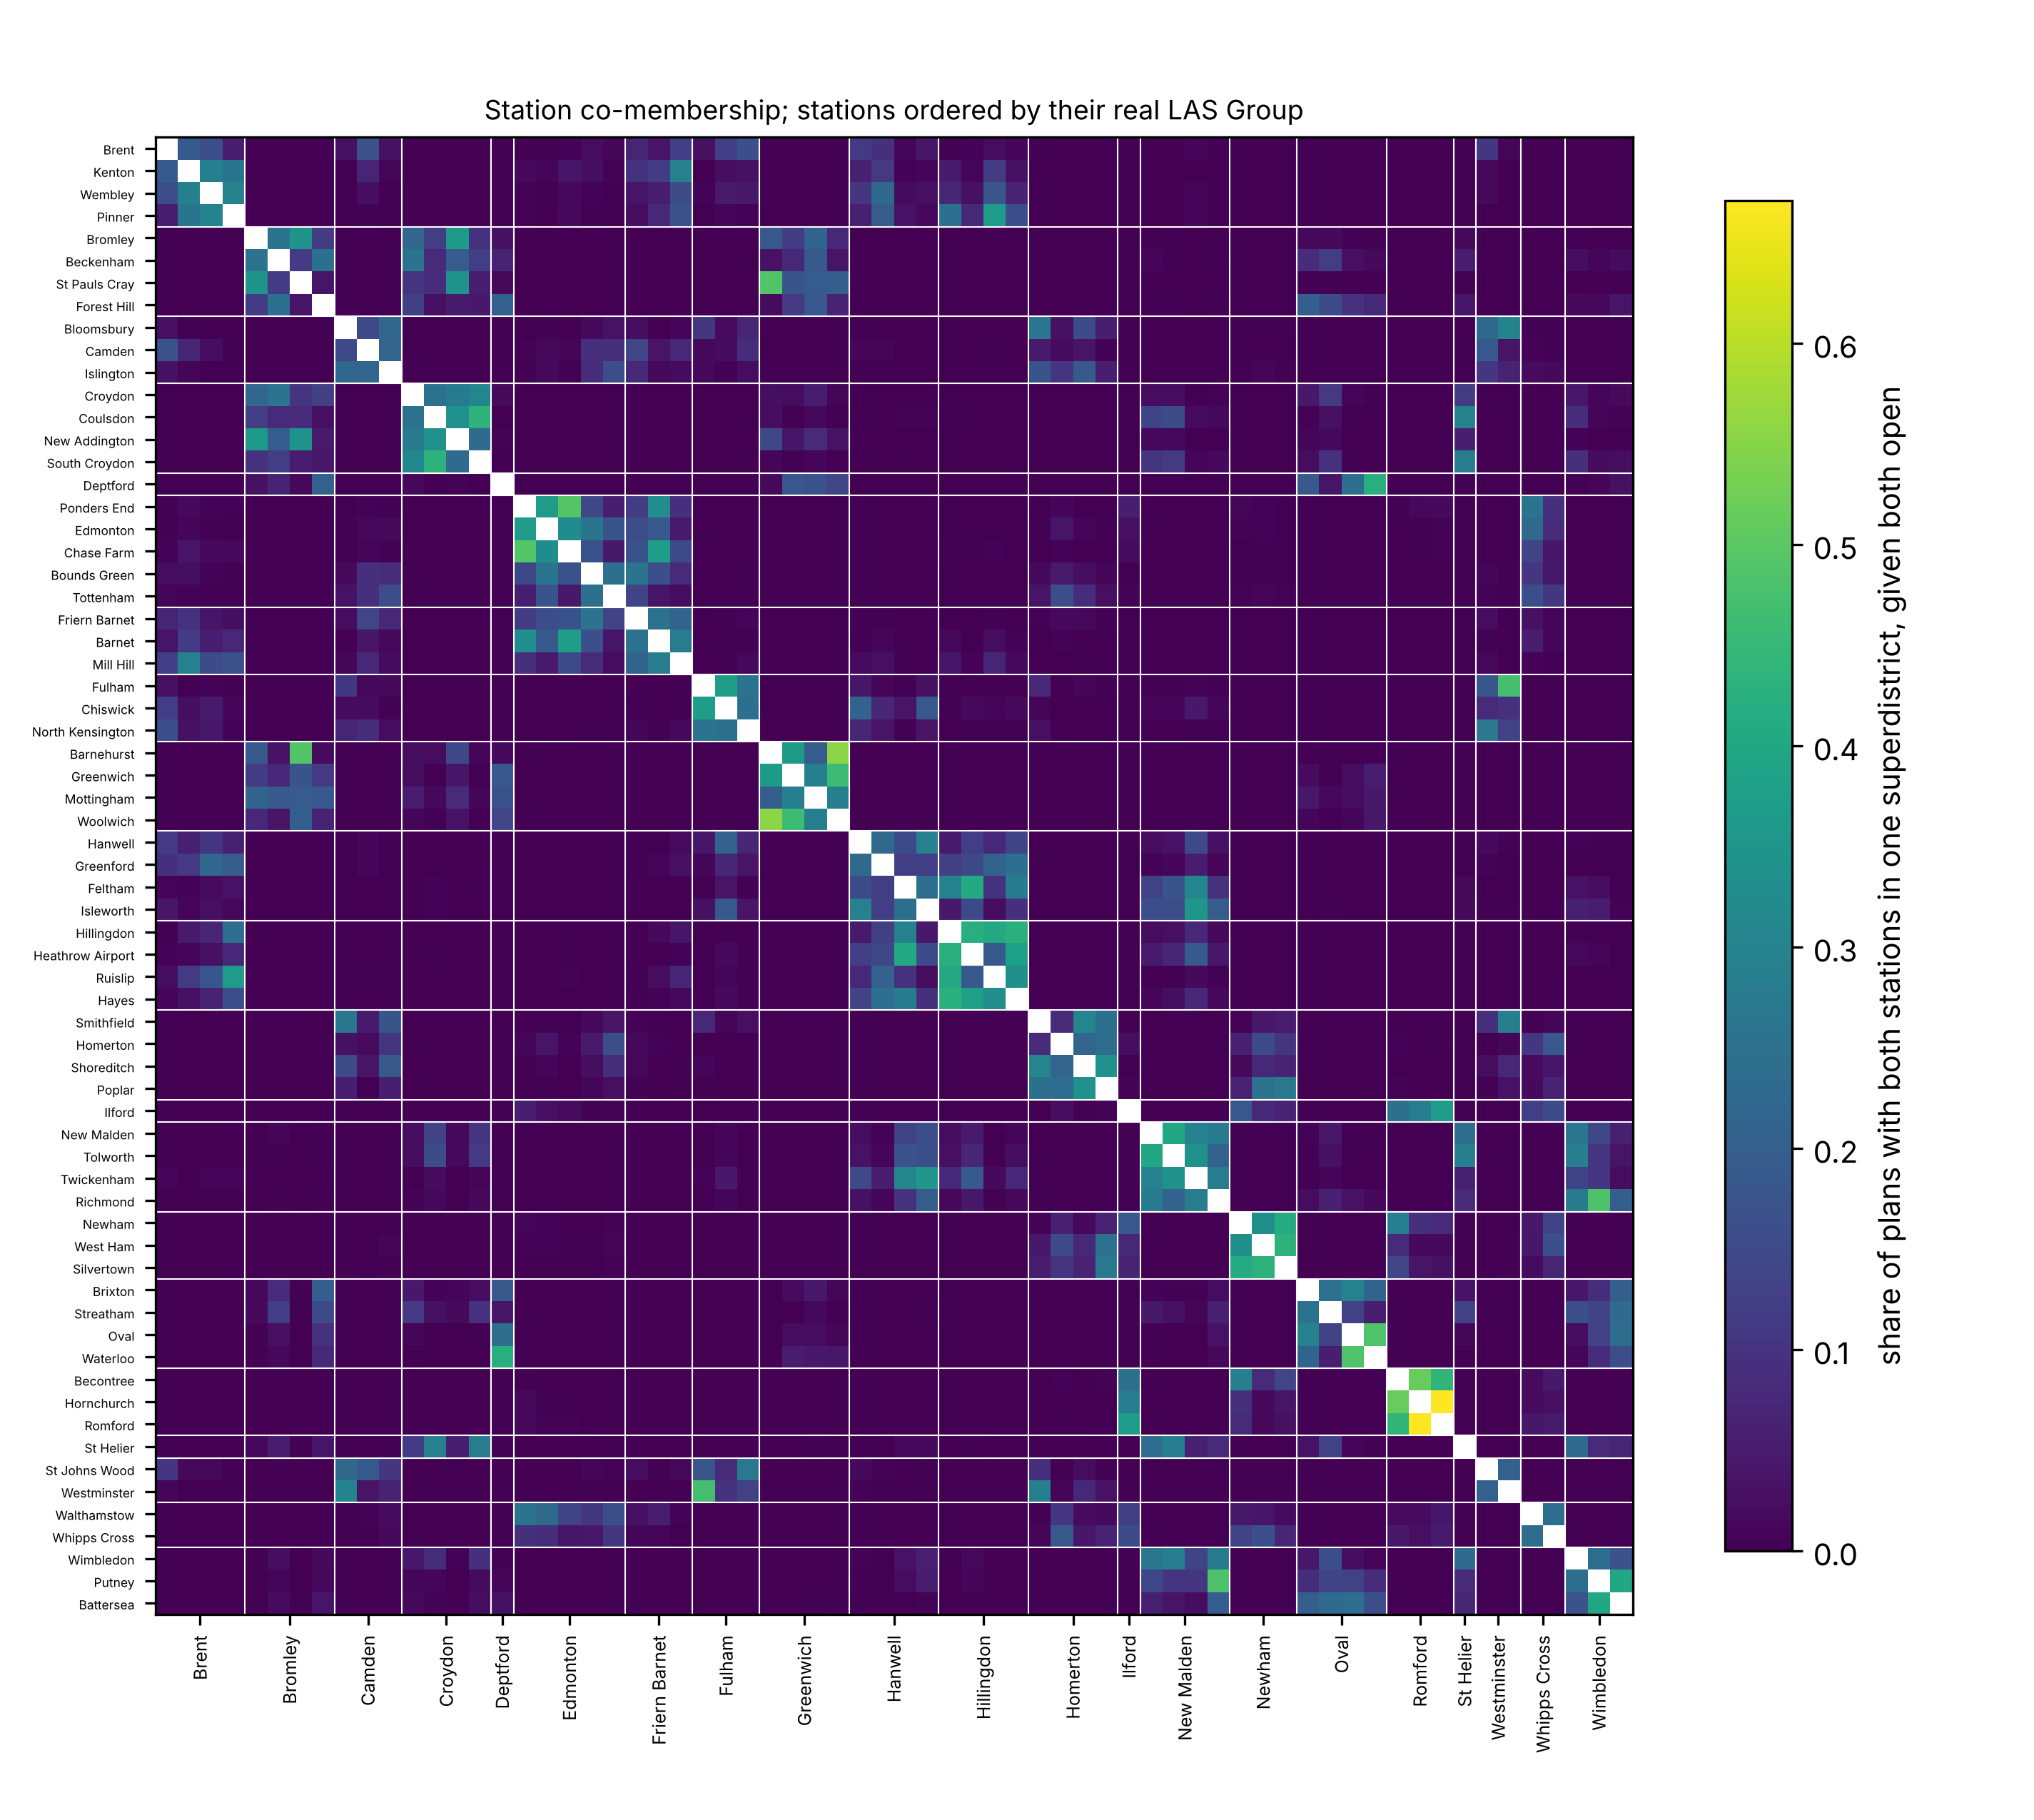
\includegraphics[width=0.7\linewidth]{figures/las/fig_groups.png}
\caption{Share of plans in which two stations belong to the same superdistrict, among the plans in which both are open; stations ordered by their real Group, with white lines separating the $21$ Groups and the colour scale running to the largest off-diagonal value.}
\label{fig:las-groups}
\end{figure}

\subsubsection{An upper bound on the price of workload balance}\label{sec:las-price}
Figure~\ref{fig:las-slas} places the operational layout in the ensemble. Its energy is $7.53$ million demand-weighted minutes, $3.08$ million on the station leg and $4.45$ million on the Group leg. That is below every one of the $6{,}400$ stored plans, whose lowest energy is $8.71$ million, below the lowest energy any chain visited after burn-in, $8.48$ million, and $22\%$ below the ensemble mean of $9.68$ million (central $90\%$ of plans between $9.21$ and $10.19$ million). Of the $2.15$ million gap to the mean, $1.13$ million is on the station leg and $1.02$ million on the Group leg. The benchmark's Group leg is computed at the documented headquarters and the ensemble's at the $1$-median of each superdistrict; computing the benchmark at its $1$-medians would widen the gap. The station-leg metrics agree with the station leg. The operational layout has a demand-weighted mean drive time of $2.9$ minutes against $4.0$ in the ensemble ($3.8$ to $4.2$), a $90$th percentile of $4.8$ minutes against $7.0$ ($6.5$ to $7.6$), and $99.5\%$ of demand within eight minutes' drive of its catchment station against $94.5\%$ ($91.8\%$ to $96.7\%$).

The source of the gap is the station loads. The operational layout opens all $66$ stations, where the sampled plans open $43$ to $61$, and its loads range from $0.19$ to $4.68$ units, a factor of $25$. Measured against the widest windows the chain can produce (Proposition~\ref{prop:effective}: $0.72$ to $1.32$ units for a one-unit station, $1.51$ to $2.56$ for two units and $2.29$ to $3.79$ for three), $20$ of the $66$ stations fall outside. Ten serve less than $0.72$ units, among them Waterloo at $0.19$ and Smithfield and Heathrow Airport at about $0.5$; Deptford, at $4.68$, exceeds the three-unit range; and nine fall between the one-unit and two-unit ranges, loads that blocks of three ambulances cannot express. Against the nominal $\pm15\%$ windows of the model the count is $36$. None of these statements depends on the sampled law.

The ensemble is a sample from a law supported on plans that satisfy these windows, so its best plan is feasible and the minimum over the feasible set lies at or below it. The distance from that plan to the operational layout is therefore an upper bound on the access cost of workload balance at this calibration, block granularity included. The layout's Group leg is evaluated at the documented headquarters and the sampled plans' at their $1$-medians, so the two sides of the total energy are not computed under one rule and the valid bound is the station-leg one, where both sides are: against the lowest station leg in the sample, $3.75$ million, it is $0.67$ million demand-weighted minutes, $22\%$ of the layout's station leg. On the total energy the gap to the best stored plan is $1.18$ million, $16\%$, which is at most the bound under a single rule. In the station-leg metrics, taking for each metric the best plan in the sample, the bound is $0.6$ minutes of mean drive time ($3.55$ against $2.92$), $1.2$ minutes at the $90$th percentile ($5.94$ against $4.78$) and $0.7$ points of eight-minute share ($98.8\%$ against $99.5\%$). Against a typical plan the differences are $2.15$ million, $1.1$ minutes and five points. The bound from the sample minimum is loose, since the chain does not seek low energy and Section~\ref{sec:exp-milp} shows that even FalCom's annealed states stay several percent above the optimum. To tighten the bound we run FalCom in the optimizer mode of Section~\ref{sec:exp-milp} on this instance, eight seeds of $50{,}000$ steps with $E$ as the objective and the calibration unchanged, $43$ to $53$ minutes per seed on one core. The annealer accepts few moves here, $616$ to $703$ per seed of which $300$ to $362$ worsen the energy, and its best plans lie between $8.23$ and $8.53$ million with a median of $8.46$ million. The best of the eight has energy $8.23$ million, $3.63$ million on the station leg, with $55$ open stations, $5.5\%$ below the lowest stored plan of the sampling runs. Against it the station-leg bound tightens to $0.55$ million, $18\%$ of the layout's station leg (its gap on the total energy is $0.70$ million, $9\%$), and in the station-leg metrics to $0.5$ minutes of mean drive time ($3.44$ against $2.92$), $1.1$ minutes at the $90$th percentile ($5.90$ against $4.78$) and $0.7$ points of eight-minute share ($98.8\%$ against $99.5\%$). The operational layout remains below every balanced plan found, and the bound remains an upper bound: a better optimizer would lower it further.
%% PHASE2-DONE
Part of this price is a limit of the demand proxy rather than of the layout. The smallest catchments sit on daytime hot spots, the West End, the City and the airport, which residential apportionment does not see. All of these are drive-time figures of a static assignment, catchment geometry rather than response performance, and the published response-time clock, which includes call handling and mobilisation, offers no validation of them. Whether the rest of the price is worth paying is an operational question that the ensemble informs but does not settle.

Nor does it depend on the within-borough apportionment, as far as a second proxy can tell. We repeat the four chains with each borough's incidents spread uniformly over its LSOAs instead of in proportion to population, the crudest alternative, with the same calibration ($97$ units) and protocol. Acceptance is $67.6\%$ to $68.2\%$ and the cross-chain Kolmogorov--Smirnov distances are $0.032$ for the energy, $0.062$ for the number of stations and $0.037$ for the cut-edge count. The plans open $52.5$ stations on average, the open frequency of a station moves by at most $0.09$ (mean $0.01$ over stations), with a single station moving by more than $0.05$, Heathrow Airport, from $41\%$ to $33\%$ once the airport's demand is spread over its borough, and the set of stations open in more than $90\%$ of plans exchanges five stations that lie within $0.03$ of the threshold under one proxy or the other (Newham, Ponders End and South Croydon leave; Chiswick and Tottenham join). Two stations of the same real Group share a superdistrict in $28\%$ of plans in which both are open and the adjusted Rand index against the real Groups is $0.28$. Under this demand the operational layout has $39$ stations outside the nominal windows and loads from $0.18$ to $4.63$ units, its energy is $7.54$ million against an ensemble mean of $9.70$ million (lowest stored plan $8.74$ million), and its mean drive time is $2.9$ minutes against $4.0$. The frequencies move, as they must when the demand surface moves, but the structure of the ensemble and the position of the layout below it do not.
%% PHASE3-DONE

The result does not depend on the tolerance. We repeat the study with $\varepsilon^1 = \varepsilon^2 = 0.25$, the widest tolerance that keeps the recursion's debt windows disjoint with margin (Claim~\ref{claim:app-unique} allows up to $2/5$), with four chains of $40{,}000$ steps and everything else unchanged. Acceptance rises to $70.0\%$ to $70.6\%$, the chains forget their starts in $400$ to $520$ steps, and the plans open $53.3$ stations on average ($47$ to $62$), $21$ of them in more than $90\%$ of plans. The run is half as long and its diagnostics are correspondingly weaker: the largest cross-chain Kolmogorov--Smirnov distance is $0.054$ for the energy, $0.053$ for the number of stations and $0.098$ for the cut-edge count, against within-chain references of $0.029$ to $0.045$, $0.024$ to $0.107$ and $0.051$ to $0.105$; split-$\hat R$ is at most $1.008$; the effective sample sizes per chain are $252$ to $438$ for the energy and $145$ to $285$ for the cut-edge count, so the $3{,}200$ stored plans are worth about $1{,}390$ and $800$ independent draws; and three of the four initial plans needed two attempts. The ensemble energy is $9.68$ million (central $90\%$ between $9.20$ and $10.20$ million, lowest stored plan $8.61$ million), within $0.1\%$ of its value at $\varepsilon = 0.15$; the mean drive time is $4.0$ minutes ($3.8$ to $4.2$) and the eight-minute share $94.4\%$ ($91.6\%$ to $96.7\%$). The operational layout still lies below every sampled plan. The wider windows admit $14$ of its $20$ out-of-window stations, but six remain outside, five below $0.56$ units and Deptford above $4.38$ (Proposition~\ref{prop:effective} at $\varepsilon = 0.25$); against the nominal $\pm25\%$ windows the count is $26$. The gap comes from the capacity model itself, in which every open station serves between $0.56$ and $4.4$ units in blocks of three ambulances, whereas the operational layout runs stations from $0.19$ to $4.68$ units. A calibration that lets a plan keep both its smallest and its largest stations needs a wider capacity range, which by Corollary~\ref{cor:app-invariant} means a larger block or the rejection-based treatment of $c \ge 4$. We leave it to future work.

\begin{figure}[!htbp]
\centering
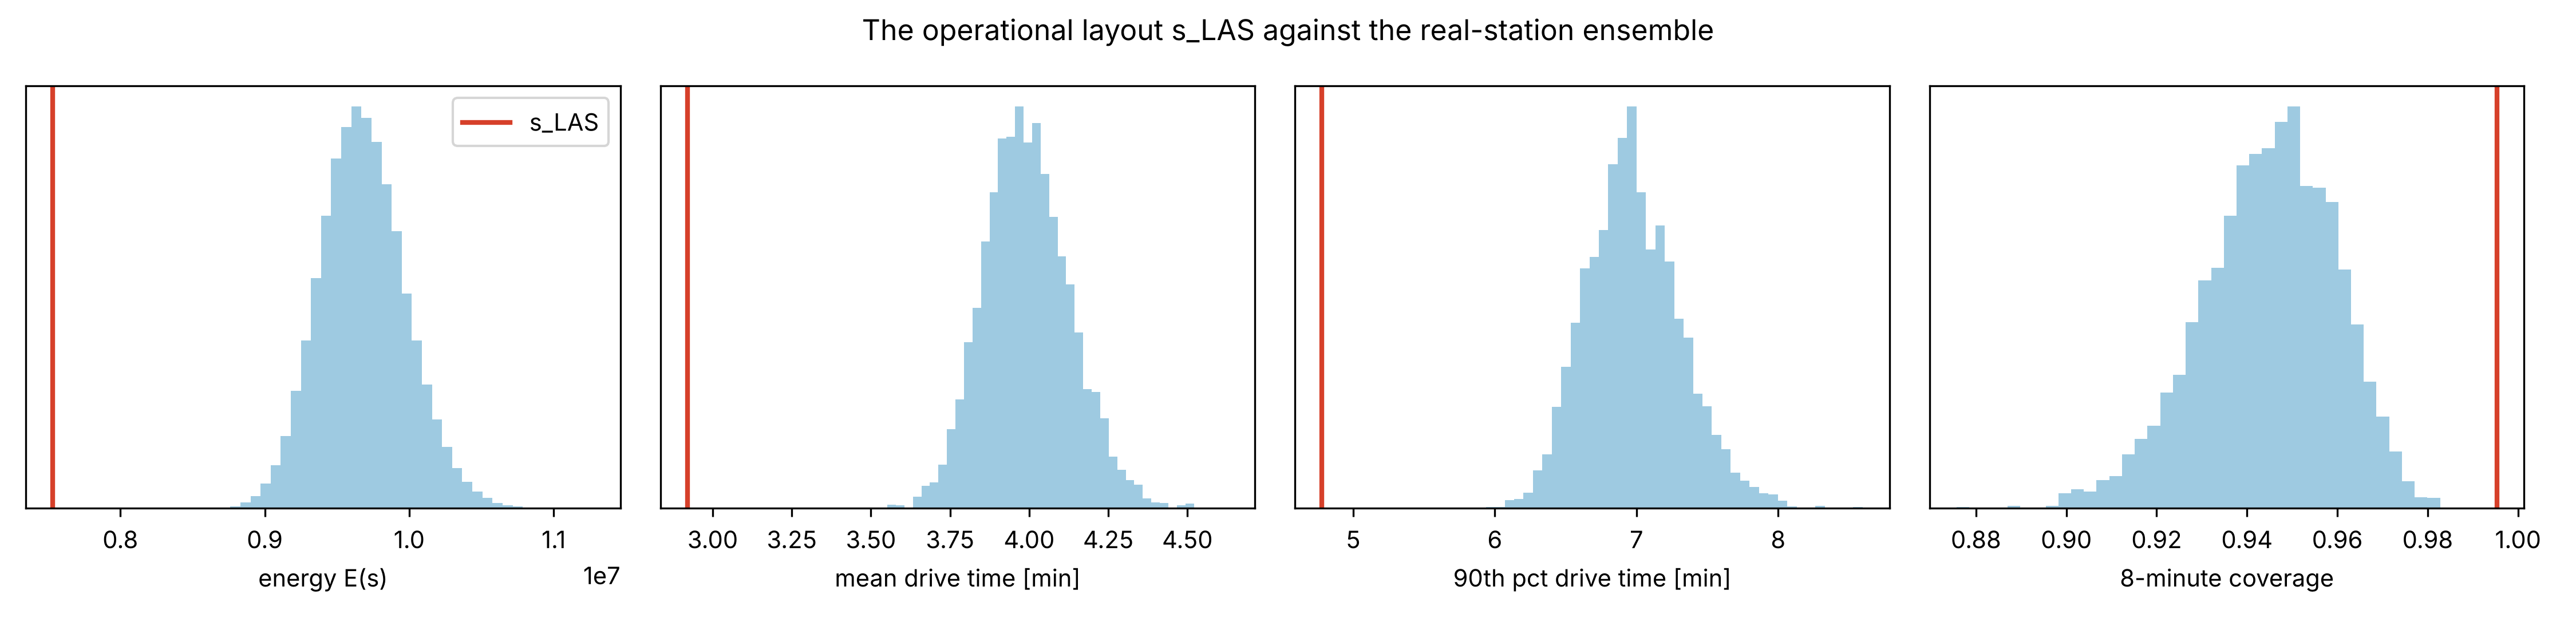
\includegraphics[width=\linewidth]{figures/las/fig_slas.png}
\caption{The operational layout $s_{\mathrm{LAS}}$ (red line) against the ensemble: energy, demand-weighted mean drive time, $90$th-percentile drive time and the share of demand within eight minutes' drive of its catchment station.}
\label{fig:las-slas}
\end{figure}

\FloatBarrier

%% -----------------------------------------------------------------------
\section{Discussion and Conclusions}
\label{sec:discussion}
%% -----------------------------------------------------------------------

This paper introduced FalCom, a recombination-type MCMC sampler for hierarchical capacitated facility location and districting problems. We summarize the main findings, discuss the limitations of the current framework, and outline extensions and directions for future research.

% =========================================================================
\subsection{Summary}
% =========================================================================

FalCom is, to our knowledge, the first sampler whose state is a hierarchy of contiguous districts with a facility and an integer capacity in every district and a number of districts that is not fixed in advance, the multiscale samplers of redistricting being its closest predecessors, and it supports ensemble-based distributional analyses. Its stationary distribution is characterized empirically rather than in closed form. On instances small enough to enumerate, the chain visits only feasible states, every one of them on the two smallest instances and all but $0.1\%$ on the third, its empirical law is independent of the start to within sampling noise (total-variation distances of $0.01$ to $0.05$ against iid floors of $0.01$ to $0.035$), and that law spreads mass across capacity mixes nearly uniformly on $12$ and $16$ units but between the uniform and spanning-tree laws on $24$, while following the spanning-tree law within a mix only loosely, at a total-variation distance of $0.11$ to $0.28$. On the London Ambulance Service, run on the $66$ real stations, five chains, four from a sector-wise start and one from a Group-based start, agree on every observable to within the noise of a single chain and forget their starts within a few hundred steps. The ensemble locates the contested and the settled service boundaries, the stations that nearly every sampled plan opens and those that many plans leave closed, and an upper bound, within a static assignment model, on the station-leg access cost that workload balance would exact from the operational layout.


% =========================================================================
\subsection{Limitations}
\label{sec:limitations}
% =========================================================================

Several limitations of the current framework should be acknowledged.



\paragraph{Mixing time.}
Section~\ref{sec:convergence} does not prove convergence, let alone bound the mixing time. The chain is validated empirically.  For political redistricting, mixing-time bounds for
ReCom-type chains remain an open problem in the Markov chain
literature~\citep{deford2021recombination}.  The hierarchical structure
of FalCom introduces additional complexity: the chain must mix at both
the supergraph and the base-graph levels.  Our convergence diagnostics
(Section~\ref{sec:exp-convergence}) provide empirical evidence that
mixing occurs within a practical number of steps, but theoretical
bounds would strengthen the guarantees.

\paragraph{Rejections at the supergraph.}
The counting predicate lets the chain run on candidate sets as sparse as
the London stations at almost no cost at the base level (fewer than one proposal in $3{,}000$ fails there), and the residual predicate removes the
supergraph strandings that capacities and counts can detect. Proposals
are still not free: on the London instance a third of them are
rejected, most of them because no pendant subtree of the sampled supergraph
tree meets its window, a tree-structural failure that the greedy
extraction cannot rule out in advance. A supergraph step that does not
extract greedily, for instance a pairwise merge-and-split move in the spirit of ReCom at level 2, is the natural next step. A pairwise move is also the route to a reversible variant with a known stationary distribution, which we leave to a follow-up paper.


% =========================================================================
\paragraph{Building a plan from scratch.}
The recursion that builds a plan from nothing is the expensive part of FalCom. Its cost grows with the number of districts a single call must extract and with the scarcity of candidate sites: a global start on the sparse grid\_50000 did not close within half an hour, at a fixed graph size the zone-wise start closes with $201$ teams but not, in twelve attempts, with twice as many (Section~\ref{sec:exp-scalability}), and at London's site density the zone-wise start on grid\_10000 needs several attempts and, for one seed in two, did not close within twelve (Section~\ref{sec:setup}). This is why the chain re-cuts only two or three superdistricts at a time and why the London plan is built sector by sector. A start that chooses its zones from the candidate layout, so that every zone has enough sites for its teams, would remove most of the attempts.

\subsection{Extensions and Future Work}
\label{sec:extensions}\label{sec:future}

Four directions follow directly from the limitations above. The first is a
\emph{reversible variant}. A pairwise merge-and-split move at the supergraph,
in the spirit of ReCom, would replace the greedy level-2 recursion whose
tree-structural failures cause the remaining rejections, and it is the natural
starting point for a Metropolis correction with a known stationary
distribution, along the lines of RevReCom~\citep{cannon2026spanning}. The
joint state would have to carry (partition, capacity, facility) at both
levels, and reversibility would have to be argued through the supergraph
projection $G^2(\mathcal{P}^1)$. The
second is \emph{deeper hierarchies}. The construction extends to $|L| > 2$ by
induction on the levels (Section~\ref{sec:outline}), but each additional level
adds a supergraph that is re-partitioned at every step, so for deep
hierarchies a schedule that re-partitions a subset of levels per step would
keep the per-step cost local. The third is \emph{uncertain demand}. Under
demand uncertainty the balance constraint~\eqref{cons:balance} may be violated by the realized demand. A robust treatment widens the tolerance to cover an uncertainty set, so that every sampled plan is feasible under all scenarios. A stochastic treatment samples demand scenarios alongside plans, which enlarges the state space and requires re-establishing its connectivity. The
fourth is the \emph{single-level and successively inclusive cases}. With
$|L| = 1$ FalCom is a capacitated sampler for districting with facility
assignment, in which an artificial upper level can serve purely as a localization device. In successively inclusive hierarchies, where a higher-level facility also provides the lower-level service, the capacity accounting of the recursion must track consumption at several levels at once. Finally, because FalCom returns an ensemble rather than an optimum, any
single plan produced by any method can be placed against that ensemble, as Section~\ref{sec:exp-emergency} does for the London layout. We expect this use, as a distributional baseline for optimization and for planning under competing criteria, to be the most common one.

\medskip

%% -----------------------------------------------------------------------
%% Bibliography
%% -----------------------------------------------------------------------
\bibliographystyle{plainnat}
\bibliography{ref_final}


\newpage

\appendix\label{app}

\section{The debt mechanism: correctness and feasibility}
\label{app:debt}

This appendix analyses the per-team debt mechanism of
Section~\ref{sec:recursive}. Let $H=(V,E)$ be a connected graph with
non-negative node demands $d\colon V\to\mathbb{R}_{\ge 0}$, aggregate
capacity $c_H\in\mathbb{Z}_{\ge 1}$, capacity bounds
$c_{\min}\le c_{\max}$ in $\mathbb{Z}_{\ge 1}$, and tolerance
$\varepsilon\in(0,1)$. Write $d_H:=\sum_{v\in V} d(v)$, let
$\bar d := d_H/c_H$ be the demand target per team and
$\tau := \varepsilon\,\bar d$ the \emph{per-team tolerance}. A district
$D$ with capacity $c(D)$ is \emph{globally balanced} when
\begin{equation}\label{eq:app-global}
  \frac{d(D)}{c(D)} \in J := [\bar d-\tau,\;\bar d+\tau].
\end{equation}

\paragraph{Recursion state.}
The recursion extracts connected districts $D_1,D_2,\ldots$ from a shrinking
residual. After $r-1$ extractions the remaining capacity is
$c^{(r)} := c_H-\sum_{j<r} c(D_j)$ (this is $c_{H^{(r-1)}}$ in the notation of Section~\ref{sec:recursive}) and the \emph{demand debt} is
\begin{equation}\label{eq:app-debt}
  \delta^{(0)} := 0,\qquad
  \delta^{(r)} := \delta^{(r-1)} + \bigl(d(D_r)-c(D_r)\,\bar d\bigr).
\end{equation}

\begin{lemma}[Telescoping]\label{lem:app-telescoping}\label{rem:telescoping}
The demand of the residual after $r-1$ extractions is
$d\bigl(H^{(r-1)}\bigr) = c^{(r)}\,\bar d-\delta^{(r-1)}$. In particular,
when the recursion closes ($c^{(k)}=0$, $H^{(k)}=\emptyset$) the debt is
$\delta^{(k)}=0$.
\end{lemma}
\begin{proof}
$d(H^{(r-1)}) = d_H-\sum_{j<r} d(D_j)
 = c_H\bar d-\sum_{j<r}\bigl(c(D_j)\bar d + d(D_j)-c(D_j)\bar d\bigr)
 = c^{(r)}\bar d-\delta^{(r-1)}$.
\end{proof}

This identity is the reason the target $\bar d$ is recomputed \emph{locally}
for every subgraph the recursion is invoked on (the merged superdistrict at
the lower level, each zone at initialization): anchoring every call to one
global average would start the recursion with $\delta^{(0)}\neq 0$.

\paragraph{The debt-clipped window.}
At step $r$ the per-team window is shifted by the debt and clipped to $J$:
\begin{equation}\label{eq:app-clip}
  \widetilde L^{(r)} := \max\{\bar d-\tau,\;\bar d-\tau-\delta^{(r-1)}\},\qquad
  \widetilde U^{(r)} := \min\{\bar d+\tau,\;\bar d+\tau-\delta^{(r-1)}\}.
\end{equation}

\begin{lemma}[Shape of the clipped window]\label{lem:app-shape}\label{cor:feas-condition}\label{cor:debt-consequences}
The clipped window has midpoint and half-width
\begin{equation}\label{eq:app-mh}
  m^{(r)} := \tfrac12\bigl(\widetilde L^{(r)}+\widetilde U^{(r)}\bigr)
           = \bar d-\tfrac12\,\delta^{(r-1)},\qquad
  h^{(r)} := \tfrac12\bigl(\widetilde U^{(r)}-\widetilde L^{(r)}\bigr)
           = \tau-\tfrac12\,\bigl|\delta^{(r-1)}\bigr|,
\end{equation}
and it is non-empty iff $|\delta^{(r-1)}|\le 2\tau$.
\end{lemma}
\begin{proof}
For $\delta^{(r-1)}\ge 0$ the clipping gives
$[\bar d-\tau,\;\bar d+\tau-\delta^{(r-1)}]$, for $\delta^{(r-1)}<0$ it gives $[\bar d-\tau-\delta^{(r-1)},\;\bar d+\tau]$. In both cases the midpoint is
$\bar d-\delta^{(r-1)}/2$ and the half-width $\tau-|\delta^{(r-1)}|/2$.
\end{proof}

\paragraph{Admissibility.}
A candidate district $D$ at capacity $c\in\{c_{\min},\ldots,c_{\max}\}$,
$c\le c^{(r)}$, is \emph{admissible} at step $r$ iff
\begin{equation}\label{eq:app-window}
  d(D)\in I^{(r)}(c) := \bigl[\,c\,m^{(r)}-h^{(r)},\; c\,m^{(r)}+h^{(r)}\,\bigr],
\end{equation}
that is, its demand lies within the \emph{same} absolute half-width
$h^{(r)}$ of the capacity-scaled midpoint $c\,m^{(r)}$ for every $c$.
(The capacity-scaled alternative $c\cdot[\widetilde L^{(r)},\widetilde U^{(r)}]$,
whose half-width grows with $c$, is discussed in Remark~\ref{rem:app-scaled}.)

\begin{theorem}[Debt evolution]\label{thm:app-evolution}\label{thm:debt-evol}\label{thm:correctness}
If $D_r$ is admissible at capacity $c=c(D_r)$, then
\begin{equation}\label{eq:app-evolution}
  \delta^{(r)}\in\Bigl[\,\bigl(1-\tfrac{c}{2}\bigr)\delta^{(r-1)}-h^{(r)},\;
                       \bigl(1-\tfrac{c}{2}\bigr)\delta^{(r-1)}+h^{(r)}\Bigr],
  \qquad h^{(r)}=\tau-\tfrac12|\delta^{(r-1)}|,
\end{equation}
and both endpoints are attained.
\end{theorem}
\begin{proof}
By \eqref{eq:app-window}, $d(D_r)-c\,\bar d\in
[\,c(m^{(r)}-\bar d)-h^{(r)},\;c(m^{(r)}-\bar d)+h^{(r)}]$ and
$c(m^{(r)}-\bar d)=-\tfrac{c}{2}\delta^{(r-1)}$ by \eqref{eq:app-mh}. Adding $\delta^{(r-1)}$ and using \eqref{eq:app-debt} gives \eqref{eq:app-evolution}. The endpoints correspond to $d(D_r)=c\,m^{(r)}\mp h^{(r)}$.
\end{proof}

\begin{corollary}[Safe capacity range]\label{cor:app-invariant}\label{cor:envelope}
If $|\delta^{(r-1)}|\le\tau$ and $c(D_r)\in\{1,2,3\}$, then
$|\delta^{(r)}|\le\tau$. Consequently, when $c_{\max}\le 3$ the recursion
started from $\delta^{(0)}=0$ satisfies $|\delta^{(r)}|\le\tau$ at every
step, and every window has half-width $h^{(r)}\ge\tau/2>0$: no window is
ever empty. For $c\ge 4$ the bound becomes $|\delta^{(r)}|\le\tau+(\tfrac{c}{2}-\tfrac32)|\delta^{(r-1)}|$, which exceeds $\tau$ as soon as the debt is non-zero, so the invariant may fail and the recursion relies on rejection.
\end{corollary}
\begin{proof}
From \eqref{eq:app-evolution},
$|\delta^{(r)}|\le|1-\tfrac{c}{2}|\,|\delta^{(r-1)}|+\tau-\tfrac12|\delta^{(r-1)}|
 =\tau+\bigl(|1-\tfrac{c}{2}|-\tfrac12\bigr)|\delta^{(r-1)}|$. For
$c\in\{1,2,3\}$ the coefficient $|1-c/2|-1/2$ equals $0,-1/2,0$, hence
$|\delta^{(r)}|\le\tau$. For $c\ge4$ it equals $c/2-3/2\ge 1/2$.
\end{proof}

\begin{corollary}[Global balance]\label{cor:app-containment}
If $|\delta^{(r-1)}|\le 2\tau$, every district admissible at step $r$ is
globally balanced: $d(D)\in I^{(r)}(c)$ implies $d(D)/c\in J$.
\end{corollary}
\begin{proof}
Write $\delta:=\delta^{(r-1)}$. From \eqref{eq:app-window},
$d(D)/c\in[\,\bar d-\delta/2-h^{(r)}/c,\;\bar d-\delta/2+h^{(r)}/c\,]$ with
$h^{(r)}=\tau-|\delta|/2$. For the upper end, if $\delta\ge0$ then
$-\delta/2+h^{(r)}/c\le h^{(r)}\le\tau$. If $\delta<0$ then
$|\delta|/2+(\tau-|\delta|/2)/c\le\tau$ because it is a convex combination of
$|\delta|/2\le\tau$ and $\tau$. The lower end is symmetric.
\end{proof}

\begin{corollary}[Closing the recursion]\label{cor:app-closing}\label{thm:feasibility}\label{thm:feas}
Let $c_{\max}\le 3$ and $|\delta^{(r-1)}|\le\tau$. In two-sided mode ($c^{(r)}\le c_{\max}$) the whole residual $H^{(r-1)}$, taken as a single district of capacity $c^{(r)}$, satisfies the balance window, and it contains a candidate because the counting predicate of Section~\ref{sec:capacitated} never lets the residual run out of them. Hence the closing step never fails on demand, and the local coverage rule $\sum_r c(D_r)=c_H$ holds; the recursion can still fail in one-sided mode through the tree draw, and the predicates of Section~\ref{sec:capacitated} rule out the doomed residuals that the candidate and count tests would otherwise reach.
\end{corollary}
\begin{proof}
By Lemma~\ref{lem:app-telescoping}, $d(H^{(r-1)})=c^{(r)}\bar d-\delta$
with $\delta:=\delta^{(r-1)}$, so
$|d(H^{(r-1)})-c^{(r)}m^{(r)}|=|{-\delta}+c^{(r)}\delta/2|
 =|\tfrac{c^{(r)}}{2}-1|\,|\delta|\le\tfrac12|\delta|$ for
$c^{(r)}\in\{1,2,3\}$, which is at most $h^{(r)}=\tau-\tfrac12|\delta|$
exactly when $|\delta|\le\tau$.
\end{proof}

A two-sided step may also split the residual into two admissible districts
of capacities $c_1+c_2=c^{(r)}$, and both sides are checked explicitly. The mirror-image symmetry $d\in I^{(r)}(c_1)\Leftrightarrow d(H^{(r-1)})-d\in I^{(r)}(c_2)$ holds for the absolute window only when $c^{(r)}=2$ or $\delta^{(r-1)}=0$. In general the complement's window is shifted by $(c^{(r)}/2-1)\,\delta^{(r-1)}$.

\begin{claim}[Unique capacity]\label{claim:app-unique}\label{claim:unique-capacity}\label{claim:disjoint}
Under $|\delta^{(r-1)}|\le\tau$, the windows $I^{(r)}(c)$ and
$I^{(r)}(c+1)$ are disjoint whenever $\varepsilon<2/5$, so every admissible subtree matches exactly one capacity.
\end{claim}
\begin{proof}
Consecutive windows are disjoint iff $m^{(r)}>2h^{(r)}$. Since
$m^{(r)}\ge\bar d-\tau/2$ and $h^{(r)}\le\tau$, it suffices that
$\bar d-\tau/2>2\tau$, i.e.\ $\varepsilon<2/5$.
\end{proof}

\paragraph{One-sided steps and the retry budget.}
In one-sided mode ($c^{(r)}>c_{\max}$) the tree-cut phase needs a
\emph{pendant} subtree of the sampled spanning tree whose demand lies in
$I^{(r)}(c)$ for some $c$ and which satisfies the candidate predicate. The
existence of such a subtree in a given tree is not guaranteed (demands of
pendant subtrees along a root-to-leaf path can jump by more than the
window width at a branching node), which is why the phase re-samples up to $M$ trees and otherwise rejects the proposal. Rejection causes are counted and reported with every experiment. Subtree demands are discrete: adding one node changes them by up to $d_{\max}:=\max_{v}d(v)$, so a window narrower than $d_{\max}$ may contain no achievable demand at all. The \emph{granularity floor} $\tau\ge d_{\max}$ keeps every window under the invariant of Corollary~\ref{cor:app-invariant} at least as wide as the heaviest node, since $2h^{(r)}=2\tau-|\delta^{(r-1)}|\ge\tau$, the grid and London calibrations satisfy it, and the enumeration instances of Section~\ref{sec:exp-enumeration} violate it and are feasible nonetheless.

\begin{remark}[Capacity-scaled window]\label{rem:app-scaled}
The alternative window $c\cdot[\widetilde L^{(r)},\widetilde U^{(r)}]$ has
half-width $c\,h^{(r)}$ and admits more cuts for $c\ge2$, but the debt
then moves by up to $c\,\tau$ per extraction: the analogue of
Corollary~\ref{cor:app-invariant} only gives $|\delta^{(r)}|\le 2\tau$ for
$c\le 2$, and for $c\ge 3$ the debt can leave the feasible envelope in one
step, after which no window is non-empty and the proposal must be
rejected. On the London instance the recursion did not close under this
window, and on a $12\times12$ test grid only 7 of 12 seeds closed at
$c_{\max}=3$ against 12 of 12 under the absolute window. FalcomChain keeps
the scaled window as \texttt{rule="scaled"} for comparison.
\end{remark}

\begin{proposition}[Necessary tolerance]
\label{thm:nec}\label{thm:lower-bound}
Let $d_{\max} := \max_{v \in V} d(v)$. If
\begin{equation}\label{eq:nec}
    \varepsilon \;<\; \frac{d_{\max}}{c_{\max}\,\bar{d}} \;-\; 1,
\end{equation}
then $H$ admits no globally balanced partition into connected districts
with capacities in $[c_{\min}, c_{\max}]$.
\end{proposition}
\begin{proof}
Let $v^\ast$ attain $d_{\max}$ and let $D^\ast$ be the district containing
it in any partition with capacities in $[c_{\min}, c_{\max}]$. Demands are
non-negative, so $d(D^\ast) \geq d_{\max}$, while global
balance~\eqref{eq:app-global} requires
$d(D^\ast) \leq c(D^\ast)\,\bar d\,(1+\varepsilon)
\leq c_{\max}\,\bar d\,(1+\varepsilon)$. Hence
$d_{\max} \leq c_{\max}\,\bar d\,(1+\varepsilon)$, the negation
of~\eqref{eq:nec}.
\end{proof}
The bound binds only when a single unit outweighs the largest admissible
district. On the London instance $d_{\max} = 1{,}526$ against
$c_{\max}\,\bar d\,(1+\varepsilon) \approx 37{,}600$, so the operative
constraint there is the granularity floor of
Section~\ref{sec:capacitated}, not this bound.

%% ----------------------------------------------------------------
\subsection*{Supergraph level}
\label{app:supergraph-correctness}\label{sec:supergraph}
%% ----------------------------------------------------------------

The supergraph recursion inherits the per-team analysis above with
three changes. The minimum number of level-1 districts per superdistrict
is $\kappa^{2}_{\min} \geq 2$, since a single-district super
collapses the hierarchy (cf.~\S\ref{sec:recursive}). The minimum
capacity is $c_{\min}^{2} = 2$. The demand target at the supergraph
level is the global average $\bar{d} = d_{G^1}/c_{G^1}$. At the base level, $\bar{d}$ is recomputed locally for the selected superdistrict so that $\delta^{(0)} = 0$ at every invocation (Remark~\ref{rem:telescoping}). The implementation disables the debt term at the supergraph level (\texttt{debt = 0}), so the corrected windows coincide with the nominal ones. The next lemma shows that demand balance is then automatic at the supergraph when the member districts were cut against the global target, with no granularity-floor condition needed there at all; under local targets the window can bind on the fringe described after the lemma. Each supernode $v$
corresponds to a level-1 district $D^1_v$, so its demand is bounded
by $d_v = d(D^1_v) \leq c_{\max}^{1}\,\bar{d}\,(1+\varepsilon^{1})$
by Corollary~\ref{cor:app-containment} at level 1.

\begin{lemma}[Supergraph balance under global targets]
\label{thm:super-feasibility}\label{cor:super-feas}\label{lem:super-convex}
Let $S$ be a superdistrict with capacity
$c(S) = \sum_{v \in S} c_v$, where supernode $v$ carries demand
$d_v = d(D^1_v)$ and weight $c_v = c^{1}(D^1_v)$. Then
\[
    \frac{d(S)}{c(S)}
    \;=\; \sum_{v \in S} \frac{c_v}{c(S)} \cdot \frac{d_v}{c_v}
\]
is a convex combination of the level-1 per-team loads. If every
level-1 district satisfies
$d_v / c_v \in \bar{d}\,[1 - \varepsilon^{1},\, 1 + \varepsilon^{1}]$
with respect to the level-2 target $\bar{d}$, then every
superdistrict, connected or not, satisfies the level-2 per-team
window whenever $\varepsilon^{2} \geq \varepsilon^{1}$, and no
granularity floor is needed at the supergraph.
\end{lemma}

\begin{proof}
A convex combination of points of an interval lies in the interval,
and $\bar{d}\,[1-\varepsilon^{1}, 1+\varepsilon^{1}] \subseteq
\bar{d}\,[1-\varepsilon^{2}, 1+\varepsilon^{2}]$ for
$\varepsilon^{2} \geq \varepsilon^{1}$.
\end{proof}

Two qualifications. First, under the local-target convention (Remark~\ref{rem:telescoping}) level-1 balance holds with respect to the local average of the region in which a district was cut rather than the global $\bar{d}$, so supernode loads lie in $\bar{d}\,[(1-\varepsilon^{1})(1-\varepsilon^{2}),\,(1+\varepsilon^{1})(1+\varepsilon^{2})]$ (Proposition~\ref{prop:effective}), and the level-2 window can bind: a union of members of one parent region $H$ has per-unit load $\bar d_H(1+\bar e)$ with $|\bar e| \le \varepsilon^1$ and $\bar d_H \in (1\pm\varepsilon^2)\,\bar d$, so its excursion outside $(1\pm\varepsilon^2)\,\bar d$ is at most $\varepsilon^1(1+\varepsilon^2)\,\bar d$ per unit. The lemma's guarantee is exact only when every member was cut against the global target, which holds for a global initial partition and for no later state of the chain. Second, the supergraph recursion carries no debt term, so Corollaries~\ref{cor:app-invariant} and~\ref{cor:app-closing} do not apply to it and nothing guarantees that it closes: by Lemma~\ref{lem:app-telescoping} the last residual has demand $c^{(k)}\bar d - \delta^{(k-1)}$ and closes only if $|\delta^{(k-1)}| \le \varepsilon^2 c^{(k)} \bar d$. A residual that violates this lies outside the window of its remaining capacity, and since in-window parts sum to an in-window whole, no spanning tree can repair it: this is a \emph{demand failure}, as opposed to the \emph{tree failure} of a residual inside its window for which the sampled trees had no admissible pendant subtree. Both end in rejection after the retry budget, and the experiments count them separately. What binds at the supergraph in practice is the discrete capacity constraints: each superdistrict must contain at least $\kappa^{2}_{\min}$ level-1 districts and carry total weight in $[c^{2}_{\min}, c^{2}_{\max}]$, and the greedy extraction could strand a final supernode that violates them. The residual predicate of Section~\ref{sec:capacitated} rules out every stranding that can be detected from capacities and supernode counts alone. The supergraph rejections that remain are tree failures or demand failures and are reported alongside the experiments.

%% ----------------------------------------------------------------
\section{Contiguity constraints of the mixed-integer model}
\label{app:shir}

We realize the closed-form $\Contiguity(x^{\ell}_{ij}, G^\ell)$ of
constraint~\eqref{cons:contiguity} via the single-commodity (SHIR) flow
reformulation of \citet{shirabe2005model}, which replaces each occurrence of
$\Contiguity(x^{\ell}_{ij}, G^1) = 1$ by a polynomial-size linear system. The
same flow argument applies at both levels because $x^{\ell}_{ij}$ assigns base
units $i \in V^1$ to facility nodes $j \in F^{\ell}$ at either level~$\ell$.
For each level $\ell \in L$, each facility $j \in F^{\ell}$, and each directed
arc $(u, v) \in A^1$ (each undirected edge of $G^1$ traversed in both
directions), introduce a non-negative flow variable $f^{\ell,j}_{uv}$. The
facility node~$j$ acts as the source of one unit of flow per assigned node,
and flow is admitted into a node only if that node is itself assigned to~$j$
at level~$\ell$:
\begin{align}
   & f^{\ell,j}_{uv} \;\leq\; |V^1|\, x^{\ell}_{vj},
   &\forall \ell \in L,\; j \in F^{\ell},\; (u,v) \in A^1
     \label{cons:shir-cap} \\
   & \sum_{\,(v,u)\in A^1} f^{\ell,j}_{vu} \;-\;
     \sum_{\,(u,v)\in A^1} f^{\ell,j}_{uv} \;=\; x^{\ell}_{uj},
   &\forall \ell \in L,\; j \in F^{\ell},\; u \in V^1 \setminus \{j\}
     \label{cons:shir-cons} \\
   & \sum_{\,(j,v)\in A^1} f^{\ell,j}_{jv} \;-\;
     \sum_{(v,j)\in A^1} f^{\ell,j}_{vj} \;=\;
     \sum_{u \in V^1} x^{\ell}_{uj} \;-\; x^{\ell}_{jj},
   &\forall \ell \in L,\; j \in F^{\ell}
     \label{cons:shir-source} \\
   & f^{\ell,j}_{uv} \;\geq\; 0,
   &\forall \ell \in L,\; j \in F^{\ell},\; (u,v) \in A^1
     \label{cons:shir-nn}
\end{align}
Constraints~\eqref{cons:shir-cap}--\eqref{cons:shir-nn} are equivalent to
$\Contiguity(x^{\ell}_{i j}, G^1) = 1$ in the binary $x^{\ell}$
projection~\citep{validi2022imposing}: at each level $\ell$ they enforce
contiguity of every service area assigned to $j$ by requiring a flow path
back to~$j$ through nodes that are themselves assigned to $j$ at level
$\ell$. Both levels reuse the same base graph $G^1$ (superdistricts inherit
adjacency from the base graph through the dual graph $G^2$), so no separate supergraph flow is needed. Level-2 contiguity becomes contiguity of the level-2 footprint on $G^1$. The runs of Section~\ref{sec:exp-milp} impose the system at level~$1$ only, which keeps the model at $O(|F^{1}|\cdot|E^{1}|)$ flow variables and capacity constraints plus $O(|F^{1}|\cdot|V^{1}|)$ conservation constraints, and check level-2 contiguity on the returned solution. Every superdistrict of every optimum reported in Table~\ref{tab:milp} is connected. The level-1 model is a relaxation of the two-level model, so an optimum of the relaxation that is feasible for the two-level model is also an optimum of the two-level model, and the values in Table~\ref{tab:milp} are optima of the model of Section~\ref{sec:model}.

\section{Optional candidate-aware cut selection}
\label{app:psi}

Sampling a subtree uniformly from $\mathcal{E}^{\ell}_{r-1}$ produces a
district that is geometrically blind to the locations of the candidate
facilities. The library therefore offers a Boltzmann-style weighting of the
admissible subtrees, the \emph{candidate-awareness score}
\begin{equation}\label{eq:awareness}
    \psi^{\ell}(T_u) = \phi^{\ell}(T_u) \cdot e^{-\gamma\,\eta^{\ell}(T_u)},
\end{equation}
where $\eta^\ell$ is a level-specific geometric penalty and $\gamma \geq 0$ an inverse temperature. At $\gamma = 0$ the score is the indicator $\phi^{\ell}$ and the selection is uniform. At the base level the penalty is the
\emph{per-capita access cost}
\begin{equation}
    \eta^1(T_u) = \hat r(T_u) \;=\; \frac{1}{d(T_u)}\,\min_{\nu \in F^1 \cap V(T_u)} \sum_{v \in V(T_u)} d_v\, \mathrm{d}(v, \nu),
    \qquad d(T_u) = \sum_{v \in V(T_u)} d_v,
\end{equation}
the demand-weighted mean distance from the best-located candidate, the demand-weighted $1$-median of $T_u$, to the units it would serve. The normalisation by $d(T_u)$ keeps $\eta^1$ comparable across cuts of different sizes, and $\eta^1$ is well defined whenever $\phi^1(T_u) > 0$. At the
supergraph level the same quantity is measured from the best-located
level-2 candidate to the base units of the subtree,
\begin{equation}\label{eq:eta-super}
    \eta^{2}(T_u) \;=\; \frac{1}{d(V^1[T_u])}\,\min_{\nu \in F^2 \cap V^1 [T_u]}\; \sum_{v \in V^1[T_u]} d_v\, \mathrm{d}\bigl(\nu,\, v\bigr),
\end{equation}
with $\eta^{2}(T_u) = +\infty$ when $F^2 \cap V^1[T_u] = \emptyset$, so that
superdistricts without a level-2 candidate vanish from the selection when
$\gamma > 0$. Larger $\gamma$ concentrates the cut distribution on subtrees
whose induced districts admit a strong demand-weighted centre, in the manner of
an inverse temperature. The weighting changes the sampled law and would have to be characterized separately. No experiment in this paper uses it.

\section{Candidate density on the grids}
\label{app:density}
%% ----------------------------------------------------------------

The grids of Section~\ref{sec:setup} have $1.5$ candidate sites per team, against $0.7$ on London. To see how much the density matters, we rebuilt grid\_1000 and grid\_10000 with $1.0$ and with $0.7$ sites per team and ran two chains of $10{,}000$ steps on each (Table~\ref{tab:density}). The chain keeps running at every density. Acceptance falls from $92\%$ to $91\%$ on grid\_1000 and from $90\%$ to $79\%$ on grid\_10000 as the density drops from $1.5$ to $0.7$ sites per team, and base-level failures stay below one proposal in $400$ ($23$ in $10{,}000$ at worst). What the density affects is the initial plan. On grid\_1000 the global recursion closes in under a second at every density. On grid\_10000 the zone-wise start closes at the first attempt in two seconds at $1.5$ sites per team, needs eight or nine attempts and $14$ to $18$ minutes at $1.0$, and at $0.7$ closes for one seed at the fifth attempt after $16$ minutes and not for the other within twelve attempts. London, at $0.7$ stations per team but with three-unit stations and sectors of about $19$ teams, starts at the first attempt, whereas the grid at $1.0$ sites per team has the same two units of candidate capacity per team but two-unit sites and zones of $25$ teams. The counting predicate keeps the chain running once it has started. Building the first plan at low density is a matter of zone size and attempts, and belongs to the initialization, not to the sampler.

\begin{table}[!htbp]
\centering
\small
\begin{tabular}{lrrrrrr}
\toprule
instance & sites per team & $|F^1|$ & acceptance & base-level failures & attempts & initialization \\
\midrule
grid\_1000  & $1.5$ & $26$ & $92\%$ & $2$ & $1$ & $<1$\,s \\
grid\_1000  & $1.0$ & $17$ & $93\%$, $93\%$ & $13$, $10$ & $1$, $1$ & $<1$\,s \\
grid\_1000  & $0.7$ & $12$ & $91\%$, $91\%$ & $13$, $21$ & $1$, $1$ & $<1$\,s \\
grid\_10000 & $1.5$ & $77$ & $90\%$ & $2$ & $1$ & $2$\,s \\
grid\_10000 & $1.0$ & $51$ & $85\%$, $86\%$ & $15$, $23$ & $9$, $8$ & $1{,}057$\,s, $833$\,s \\
grid\_10000 & $0.7$ & $36$ & $79\%$ & $17$ & $5$, none in $12$ & $964$\,s \\
\bottomrule
\end{tabular}
\caption{Candidate density on two grids: two seeds of $10{,}000$ steps at each density, one value per seed where the seeds differ. Base-level failures are proposals whose level-1 recursion did not close within its retry budget, per $10{,}000$ proposals. Attempts count the zone-wise (grid\_10000) or global (grid\_1000) recursions needed for the first plan, and initialization is the time of the successful one. The $1.5$ rows are the chains of Section~\ref{sec:exp-scalability}.}
\label{tab:density}
\end{table}

\section{LAS data assembly and the benchmark state}
\label{app:slas}
%% ----------------------------------------------------------------

\paragraph{Data assembly.}
The catchment file holds $5{,}042$ LSOAs on 2021 boundaries from the ONS Open Geography Portal. The $48$ in Brentwood, Essex, served by the East of England Ambulance Service, are excluded, leaving $4{,}994$ with a mean population of about $1{,}820$. The station roster is the $66$ active stations of the LAS estate, compiled from a published station list and cross-referenced with the freedom-of-information pages of the LAS website and with OpenStreetMap, with coordinates geocoded from postcodes; the closed station N4 Lee is excluded. Demand is the 2010 to 2015 mean of the monthly incident totals that LAS publishes by borough~\citep{las_incidents}, a London Datastore release covering June 2009 to July 2016 from which one mislabelled month is dropped, about $1.056$ million incidents a year across the $33$ boroughs, all of them in the catchment, apportioned to the LSOAs of each borough in proportion to the ONS mid-2024 small-area population estimates on 2021 LSOA boundaries~\citep{ons_sape2024} by the largest-remainder method, so that demands are integers and borough totals are preserved exactly. Variation between boroughs is therefore observed and variation within a borough is a proxy: daytime hot spots such as hospitals, rail termini and the West End are smoothed into their residential surroundings. The inputs span fifteen years, 2010 to 2015 incidents, mid-2024 population estimates and a 2024/25 productivity target. Travel times are shortest-path driving times on the Greater London OpenStreetMap road network, computed with the \texttt{falcomtravel} library from every station to every LSOA centroid, with free-flow speeds scaled by $1.6$ to represent driving under lights and sirens. The factor is an assumption, not a calibrated value, and affects absolute drive times only. Four LSOAs, isolated fragments of the network, cannot be reached from any station by the routing engine (Hillingdon 031A, Newham 034A, Bromley 018F and Camden 026E; $264$ station and LSOA pairs, $0.1\%$ of demand, none of them hosting a station); for these, straight-line distance at $25$ km/h is used. All drive times are station-to-centroid times. They exclude call handling and mobilisation and are not comparable with the published response-time clock.

\paragraph{The benchmark state.}
No vector boundaries of the sectors or Groups are published. The August 2023 operational estate map, a raster image that LAS released in response to Freedom of Information request 6055~\citep{las_estate2023}, and the 2025 list of departments~\citep{las_departments2025}, which lists the stations of each Group, together define
the five sectors administratively as unions of London boroughs, the
five NHS England Integrated Care Systems for London (NCL, NEL, NWL,
SEL, SWL). We assign each LSOA to its sector via the borough lookup
($32$ London boroughs plus the City of London, the latter grouped
into the City~\&~Hackney pair in NE). At the Group level, the list of departments partitions each sector's boroughs among $3$--$5$
Groups, and $4{,}486$ LSOAs ($89.8\%$) inherit their Group directly from this borough lookup. In three boroughs (Hounslow, Lambeth, Lewisham), the official 2023 Operational Estate map's dashed Group boundaries cut across the borough, splitting it between two Groups. Each of the $425$ LSOAs ($8.5\%$) inside such split boroughs inherits the Group of its nearest LAS station drawn from the two candidate Groups. A final $83$ LSOAs ($1.7\%$) are explicit
corrections from visual cross-check against the August-2023 raster
where neither the borough nor the within-borough Voronoi heuristic
matched the official dashed line. Contiguity of every resulting
Group region was verified directly on the rook-adjacency graph
$G^1$. Each station belongs to the Group of the LSOA it sits in, and within each Group every LSOA is assigned to its nearest station by straight-line (British National Grid) distance, which yields the $66$ station catchments of $s_{\mathrm{LAS}}$. Three of these catchments (Forest Hill, Isleworth, Richmond) come out in two or three pieces on $G^1$, where the straight-line rule jumps a bend of the Thames or a railway corridor. The $17$ LSOAs of the detached pieces, $0.3\%$ of demand, are reassigned to the neighbouring station of the same Group with which they share the most rook edges (Beckenham, Hanwell, Feltham and Twickenham), after which every catchment and every Group induces a connected subgraph. The moves are listed with the data (\texttt{lsoa\_to\_station\_contiguity\_moves.csv}).



\end{document}